\documentclass[twocolumn,prc,showpacs,nofootinbib,preprintnumbers,amsmath,amssymb,superscriptaddress]{revtex4-1}
%\documentclass[twocolumn,prc,preprint,showpacs,preprintnumbers,amsmath,amssymb,superscriptaddress,a4paper,nofootinbib]{revtex4-1}

\usepackage{times}
\usepackage{natbib}
\usepackage{amssymb,amsbsy,amsmath,amsfonts}
\usepackage{graphicx}% Include figure files
\usepackage{epsf,epsfig,float,latexsym,amsthm,fancyhdr,rotating}
\usepackage{graphics,psfrag,longtable}
%\usepackage{srcltx}
\usepackage{slashed}
%\usepackage{footnote}
\usepackage[colorlinks,citecolor=blue,linktoc=all,linkcolor=cyan]{hyperref}
\usepackage{upgreek}
 
\def\hpm{\hphantom{-}}
\def\beq{\begin{equation}}
\def\eeq{\end{equation}}
\def\bea{\begin{eqnarray}}
\def\eea{\end{eqnarray}}
\def\beqa{\begin{equation}\begin{array}{l}}
\def\eeqa{\end{array}\end{equation}}
% labels
\def\eqlab#1{\label{eq:#1}}
\def\figlab#1{\label{fig:#1}}
\def\tablab#1{\label{tab:#1}}
\def\seclab#1{\label{sec:#1}}
% reference
\def\eref#1{(\ref{eq:#1})}
\def\Eqref#1{Eq.~(\ref{eq:#1})}
\def\figref#1{fig.~\ref{fig:#1}}
\def\fref#1{\ref{fig:#1}}
\def\Figref#1{Fig.~\ref{fig:#1}}
\def\tabref#1{\ref{tab:#1}}
\def\Tabref#1{Table \ref{tab:#1}}
\def\secref#1{Section \ref{sec:#1}}
% vectors
\def\sla#1{#1 \hspace{-2mm} \slash}
\def\slap{p \hspace{-2mm} \slash}
\def\slad{\partial \hspace{-2.2mm} \slash}
\def\slaP{P \!\!\!\! \slash}
% fractions
\def\boxfrac#1#2{\mbox{\small{$\frac{#1}{#2}$}}}
\def\half{\mbox{$\frac{1}{2}$}}
\def\sfrac#1{\mbox{\small{$\frac{1}{#1}$}}}
\def\thalf{\mbox{\small{$\frac{3}{2}$}}}
\def\quarter{\mbox{$\frac{1}{4}$}}
\def\third{\mbox{$\frac{1}{3}$}}
\def\sixth{\mbox{$\frac{1}{6}$}}

% matrices
\def\barr{\left(\begin{array}{c}}
\def\earr{\end{array}\right)}
\def\bmat{\left(\begin{array}{cc}}
\def\emat{\end{array}\right)}
%--------------------------------------------
% symbols
\def\al{\alpha}
\def\be{\beta}
\def\ga{\gamma} \def\Ga{{\it\Gamma}}
\def\de{\delta} \def\De{\Delta}
\def\veps{\varepsilon}  \def\eps{\epsilon}
\def\kp{\kappa}
\def\la{\lambda} \def\La{{\Lambda}}
\def\Pit{{\it\Pi}}
\def\Psit{{\it\Psi}}
\def\si{\sigma} \def\Si{{\it\Sigma}}
\def\th{\theta} \def\vth{\vartheta} \def\Th{\Theta}
\def\w{\omega} \def\W{\Omega} \def\hw{\hat{\omega}}
\def\vfi{\varphi}\def\vphi{\varphi}
\def\z{\zeta}
\def\bra{\langle} \def\ket{\rangle}

\def\pa{\partial}
\def\vrho{\varrho}
\def\barf{\zeta}
\def\ie{{i.e., }}
\def\eg{{e.g.\ }}
\def\cl{\centerline}
\def\ni{\noindent}
\def\pa{\partial}
\def\ra{\rightarrow}
\def\nn{\nonumber}
\def\dd{\mathrm{d}}
\def\cO{\mathcal{O}}
\def\DD{{\mathcal D}}
\def\lag{{\mathcal L}}
\def\ham{{\mathcal H}}
\def\aa{\mathcal{a}}
\def\kk{\mathcal{k}}
%\def\gg{\mathcal{g}}
\def\xx{\mathscr{x}}
\def\yy{\mathscr{y}}
\def\zz{\mathscr{z}}
\def\MM{\mathcal{M}}
\def\MA{{\mathcal A}}
\def\MR{{\mathcal R}}
\def\MQ{{\mathscr q}}
\def\MB{{\mathcal B}}
\def\MP{{\mathcal P}}
\def\TT{{\mathscr T}}
\def\ZZ{\mathcal{Z}}
\def\rZ{\mathantt{Z}}
\def\zZ{\mathpzc{Z}}



\def\bGa{{\bf\Gamma}}
\def\bS{{\bf S}}
\def\psib{\bar{\psi}} \def\Psib{\bar{\Psit}}
\def\pib{\bar{\pi}} \def\Pib{\bar{\Pi}}
\def\xib{\bar{\xi}}

\DeclareMathOperator\arctanh{arctanh}
\DeclareMathOperator\im{Im}
\DeclareMathOperator\re{Re}\def\3d{3-D}
\def\CMS{CMS}
\def\ODI{O$\Delta$I}
\def\ODR{O$\Delta$R}
\newcommand{\lsim}{\, \, \raisebox{-0.8ex}{$\stackrel{\textstyle <}{\sim}$ }}
\def\ol#1{\overline{#1}}
\def\amm{a.m.m.}
%---------------------------------
\def\hate{\hat{\mathbf{e}}}
\def\bq{\mathbf{q}}
\def\bvare{\boldsymbol{\varepsilon}}
\def\bsig{\boldsymbol{\sigma}}


\textwidth18.5cm
\begin{document}
%\preprint{MITP/13-042}
\title {Complete next-to-next-to-leading-order calculation of
the nucleon doubly-virtual Compton scattering  in baryon chiral perturbation theory}
\author{Jose Manuel Alarc\'on}
%\affiliation{
%Cluster of Excellence PRISMA Institut f\"ur Kernphysik, Johannes Gutenberg-Universit\"at, Mainz D-55099, Germany}
\affiliation{Theory Center, Thomas Jefferson National Accelerator Facility, \\
12000 Jefferson Avenue, Newport News, VA 23606, USA}
\author{Franziska Hagelstein}
\affiliation{Albert Einstein Center for Fundamental Physics, Institute for Theoretical Physics, University of Bern, Sidlerstrasse 5, CH-3012 Bern, Switzerland}
\author{Vadim Lensky}
\affiliation{Institut f\"ur Kernphysik \&  Cluster of Excellence PRISMA,
 Johannes Gutenberg-Universit\"at  Mainz,  D-55128 Mainz, Germany}
\affiliation{Institute for Theoretical and Experimental Physics, Bol'shaya Cheremushkinskaya 25, 117218 Moscow, Russia}
\affiliation{National Research Nuclear University MEPhI (Moscow Engineering Physics Institute), 115409 Moscow, Russia}
\author{Vladimir Pascalutsa}
\affiliation{Institut f\"ur Kernphysik \&  Cluster of Excellence PRISMA,
 Johannes Gutenberg-Universit\"at  Mainz,  D-55128 Mainz, Germany}
 \email{vladipas@kph.uni-mainz.de}

\begin{abstract}
We calculate the generalized polarizabilities and moments of the nucleon structure functions in the manifestly-covariant  baryon chiral perturbation theory (BChPT) to next-to-leading order (NLO). 
This calculation is a NLO prediction of the non-Born doubly-virtual Compton scattering (VVCS) off the nucleon.
By expanding our results in powers of the inverse nucleon  mass
we reproduce the known `heavy-baryon' expressions.  The results for the
forward spin polarizability, $\gamma_0$, and the longitudinal-transverse polarizability, $\delta_{LT}$,
of the proton are compared with the existing expressions, while the results
for the scalar polarizabilities are new. The latter play an
important role in the calculation of nucleon structure 
effects in the muonic-hydrogen Lamb shift. 
The result for $\delta_{LT}$ of the neutron
is in much better agreement with experiment than 
the corresponding heavy-baryon result, which means
the so-called ``$\delta_{LT}$ puzzle" could be explained
by relativistic effects.
\end{abstract}
%\pacs{}
\date{\today}
\maketitle

\tableofcontents

\section{Introduction}

The polarizabilities of the nucleon fully characterize its two-photon response
at low energies and, hence, are important for studies of nucleon structure,
most notably for the determination of the proton charge radius from
either atomic spectra or elastic electron scattering. As the ``proton
charge radius puzzle" \cite{Pohl:2010zza,Antognini:1900ns,Pohl:2013yb,Hagelstein:2015egb} is yet to 
see a fully satisfactory explanation, 
an accurate knowledge of nucleon polarizabilities and of their role
in the two-photon-exchange physics is ever more relevant. 

In this work, we obtain the momentum-transfer ($Q^2$) behavior of the
generalized nucleon polarizabilities of the doubly-virtual Compton scattering (VVCS)
process in the forward direction at next-to-leading order (NLO) in Baryon
Chiral Perturbation Theory (BChPT) including the $\Delta(1232)$ degrees of freedom.  Our results for the scalar
polarizabilities are new, while the ones for the forward spin polarizability, $\gamma_0$, and the longitudinal-transverse polarizability, $\delta_{LT}$,
are compared with the recent results of
Bernard {\it et~al.}~\cite{Bernard:2012hb}. 
Upon expanding our results in powers of inverse nucleon mass, $M_N^{-1}$, we are able to reproduce the LO results
of Heavy-Baryon Chiral Perturbation Theory (HBChPT) 
which exist for the magnetic polarizability \cite{Birse:2012eb} 
and the forward spin polarizabilities~\cite{Kao:2002cp}.

%In the manifestly-invariant formulation of BChPT one 

The HB results can always be obtained by an expansion
of the BChPT results in powers of inverse nucleon mass and, hence, are easily available. We, however, do not see a rationale to drop the higher-order $M_N^{-1}$ terms when they are not 
negligible (i.e., when their actual size exceeds by far the natural estimate
for the size of higher-order terms).

The interest on the proton polarizabilities has increased since the experimental determination of the proton radius from muonic hydrogen ($\mu$H) \cite{Pohl:2010zza,Antognini:1900ns} has determined a value which is at present $5.6\,\sigma$ away from the value determined from normal hydrogen ($e$H) spectroscopy and $ep$ scattering \cite{Bernauer:2010wm}, as averaged in the CODATA '14 review \cite{Mohr:2015ccw}. The $\sim 300$~$\upmu$eV disagreement between the Lamb shift measurements in $\mu$H and $e$H could be due to the internal electromagnetic structure of the proton, because the muon in $\mu$H is orbiting much closer to the proton and is much more influenced by its internal electromagnetic structure than the electron in $e$H. For the Lamb shift, the scalar dipole polarizabilities are of interest, while the planned measurements of the ground-state hyperfine splitting in $\mu$H \cite{Pohl:2016xsr} will bring the spin polarizabilities to the center of attention.

Polarizabilities can be accessed through experimental information by means of different sum rules that involve the cross sections of the inclusive photoabsorption processes \cite{Drechsel:2002ar,Hagelstein:2015egb}. 
For example, for real forward Compton scattering the Baldin sum rule \cite{BaldinSumRule} connects the sum of electric and magnetic dipole polarizabilities to the total photoabsorption cross section $\sigma_T$. The GDH sum rule \cite{Gerasimov:1965et,Drell:1966jv} relates the anomalous magnetic moments of the nucleon to the helicity-difference photoabsorption cross section $\sigma_{TT}$. This has been subject of several experiments at MAMI (Mainz) and ELSA (Bonn) some years ago \cite{Ahrens:2001qt, Helbing:2002eg}.
These sum rules can be generalized to the virtual photon case \cite{Drechsel:2002ar}, where the virtual photon produced in the electroproduction process acts as a probe whose resolution depends on its virtuality $Q^2$. In this way, one obtains information about the density of polarization inside the nucleon.

%IR, EOMS, in fact there is nothing to renormalize, let alone regularize
%in the leading-order polarizability calculation as is especially evident from the validity of the sum rules.
%
%Indeed we check that the tree-level cross sections of pion electro-production reproduce the result of the direct calculation via the VVCS amplitude.
%
%Prediction!

This work is considered to be an extension of Ref.~\cite{Lensky:2014dda}.
Here, we compute the VVCS amplitude in BChPT to make parameter-free predictions for the polarizabilities of the proton and neutron at NLO, where we now include also the Coulomb coupling $g_C$ at the $\gamma^*N \Delta$ vertex.
As we will show in Sec.~\ref{Sec:Scalar-Pol}, we predict the high-$Q^2$ behavior of the polarizabilities, which allows to compute the two-photon-exchange polarizability corrections to the $\mu$H Lamb shift \cite{Alarcon:2013cba}. \textcolor{red}{We also provide, for the first time in the literature, a calculation of the longitudinal polarizability $\alpha_L(Q^2)$ and a prediction for the $Q^2$-dependence of the scalar polarizabilities in the framework of covariant BChPT. Also, we provide a more detailed comparison to the calculation of Bernard {\it et~al.}~\cite{Bernard:2012hb}, focusing in particular on the longitudinal-transverse polarizability of the proton $\delta_{LT}^{p}(Q^2)$.}

This paper is organized as follows: In Sec.~\ref{Sec:Formalism}, we develop the formalism we use to make our calculations. In Secs.~\ref{Sec:Scalar-Pol}-\ref{Sec:GeneralizedGDH}, we show our results for the proton and neutron polarizabilities and some interesting moments of their structure functions. Finally, Sec.\ \ref{Sec:Summary}, we summarize the results obtained herein, comment on the improvements done with respect to previous calculations, and give an outlook to future applications. In the appendices, we analyze some technical details involved in the calculations and show  analytical results for the tree-level pion-production photoabsorption cross sections (App.~\ref{App:CrossSections}) and the contributions of the pion-cloud and the $\Delta$-exchange to the polarizabilities and their slopes at the real photon point (App.~\ref{App:Polarizabilities}). 
\begin{widetext}
\section{Formalism} 
\label{Sec:Formalism}
The forward VVCS amplitude can be parametrized by four 
scalar functions ($f_i$ and $g_i$):
\begin{align}\label{Eq:T-Compt-definition}
T(\nu,Q^2)=f_{L}(\nu,Q^2) +(\vec{\epsilon}^{\, \prime *} \cdot \vec{\epsilon}\,) \,f_{T}(\nu,Q^2)  +  i \vec{\sigma}\cdot (\vec{\epsilon}^{\, \prime *} \times \vec{\epsilon}\,)\, g_{TT}(\nu,Q^2) -  i \vec{\sigma}\cdot [(\vec{\epsilon}^{\, \prime *} - \vec{\epsilon}\,)\times \hat{q}]\, g_{LT}(\nu,Q^2), 
\end{align}
where $\epsilon$ ($\epsilon^*$) is the incoming (outgoing) photon polarization vector, $q$ is the photon four-momentum, $Q^2=-q^2$ is the virtuality of the photon and $\nu=(s-M_N^2+Q^2)/2M_N$ is the energy of the photon in the lab system.
The energy variable $\nu$ is frequently used for applications of dispersive methods because it is odd under crossing, $\nu \to -\nu$.
\end{widetext}

Two of the scalar VVCS functions are independent of the spin ($f_T$ and $f_L$), while the other two ($g_{TT}$ and $g_{LT}$) are spin-dependent. 
In the real photon case ($Q^2=0$), the functions that involve longitudinal polarization ($f_L$ and $g_{LT}$) vanish, and only $f_T$ and $g_{TT}$ survive. 
Low, Gell-Mann and Goldberger \cite{LET} proved in the 50's that the leading terms of the low-energy expansions are determined uniquely by the global properties of the system: charge, mass and anomalous magnetic moment. 
The polarizabilities enter as higher-order corrections. They are related to the internal structure of the nucleon, which can be accessed through photoabsorption experiments (see Sec.~\ref{Sec:ConnectionWithElectroproduction}).


\vfill\null
%\columnbreak
Constructed from crossing symmetry, Lorentz and gauge invariance, one can deduce the general structures: 
\begin{subequations}
\eqlab{fgFunctions}
\begin{eqnarray}
  f_T(\nu, Q^2))&=& f_T^{(B)}(\nu, Q^2)\nn\\
 &+&4\pi\left[ Q^2 \beta_{M1} +(\alpha_{E1} + \beta_{M1}) \nu^2\right] + \dots \label{Eq:LEX-fT}\\
  f_L(\nu, Q^2)&=& f_L^{(B)}(\nu, Q^2) + 4 \pi(\alpha_{E1}+\alpha_{L} \nu^2) Q^2 + \dots \qquad \label{Eq:LEX-fL}\\
  g_{TT}(\nu, Q^2)&=&g^{(B)}_{TT}(\nu, Q^2) + 4 \pi\gamma_0  \nu^3 + \dots \label{Eq:LEX-gTT}\\
  g_{LT}(\nu, Q^2)&=&g^{(B)}_{LT}(\nu, Q^2) +  4 \pi\delta_{LT} \nu^2 Q + \dots \label{Eq:LEX-gLT}
\end{eqnarray}
\end{subequations}
\newpage
where the Born terms are \cite{Drechsel:2002ar}:
\begin{subequations}
\begin{align}
 & f_T^{(B)}(\nu, Q^2) =  - \frac{4\pi \alpha_{\rm em}}{M_N} \Big( F_D^2 + \frac{\nu_B^2 G_M^2}{\nu^2-\nu_B^2} \Big), \label{Eq:BT-fT}\\
  &  f_L^{(B)}(\nu, Q^2) = - \frac{\pi \alpha_{\rm em} Q^2}{ M_N^3} \Big( F_P^2 + \frac{4M_N^2 G_E^2}{\nu^2-\nu_B^2} \Big), \label{Eq:BT-fL}\\
 & g^{(B)}_{TT}(\nu, Q^2) = - \frac{2\pi \alpha_{\rm em} \nu}{ M_N^2} \Big( F_P^2 + \frac{Q^2 G_M^2}{\nu^2-\nu_B^2} \Big), \label{Eq:BT-gTT}\\
 & g^{(B)}_{LT}(\nu, Q^2) =  \frac{2 \pi\alpha_{\rm em} Q}{M_N^2} \Big( F_D F_P - \frac{Q^2 G_E G_M }{\nu^2-\nu_B^2} \Big), \label{Eq:BT-gTL}
\end{align}
\end{subequations}
with $\alpha_{\rm em}$ the fine structure constant, $G_E(Q^2)$ and $G_M(Q^2)$ the electric and magnetic Sachs form factors, and $\nu_B=Q^2/2M_N$. Note that the Sachs form factors are related to the Dirac and Pauli form factors in the following way:
\begin{subequations}
\begin{align}
& G_E(Q^2)=F_D(Q^2) - \frac{Q^2}{4M_N^2} F_P(Q^2),\\
& G_M(Q^2)=F_D(Q^2) + F_P(Q^2).
\end{align}
\end{subequations}


\textcolor{red}{The prefactors of the $\nu$ expansion in \Eqref{fgFunctions}, $\alpha_{E1}$, $\beta_{M1}$, $\alpha_{L}$, $\gamma_{0}$ and $\delta_{LT}$, are $Q^2$ dependent functions.}
They  are the so-called generalized polarizabilities (GP), which generalize the response of the nucleon to the case of finite momentum transfer. Notice that $\alpha_L$ is usually defined including the $Q^2$ proportionality that stems from gauge invariance. 
In this case, we think it is more natural to take the $Q^2$ term out of the definition, as is usually done with $Q$ in $\delta_{LT}$.

In a covariant approach, as the one we follow in this work, the Compton tensor in the forward limit has the following tensor decomposition \cite{Hagelstein:2015egb}:
\begin{widetext}
%\begin{align}\label{Eq:T-Rel}
%T(\nu,Q^2) = \epsilon_{\mu}^{\prime *} \epsilon_\nu \Bigg\{  \Big( -g^{\mu \nu} + \frac{q^\mu q^\nu}{q^2} \Big) T_1(\nu,Q^2) + \frac{1}{M_N^2} \Big(  p^\mu - \frac{p\cdot q}{q^2} q^\mu \Big) \Big(  p^\nu - \frac{p\cdot q}{q^2} q^\nu \Big) T_2(\nu,Q^2) \nonumber \\ 
%                  +  \frac{i}{M_N} \epsilon^{\mu \nu \alpha \beta} q_\alpha s_\beta S_1(\nu,Q^2)   +\frac{i}{M_N^3} \epsilon^{\mu \nu \alpha \beta} q_\alpha (p\cdot q  s_\beta -s\cdot q  p_\beta ) S_2(\nu,Q^2)      \Bigg\}, 
%\end{align}
%where $s^\mu$ is the covariant spin tensor which satisfy $s\cdot p=0$ and $s^2=-1$, and the normalization of the Levi-Civita tensor is $\epsilon_{0123}=+1$. 
\bea
\label{Eq:T-Rel}
\hspace{-0.5cm}T(\nu,Q^2) & = &  \epsilon_{\mu}^{\prime *} \epsilon_\nu \Bigg\{ 
\left( -g^{\mu\nu}+\frac{q^{\mu}q^{\nu}}{q^2}\right)
T_1(\nu, Q^2) +\frac{1}{M^2} \left(p^{\mu}-\frac{p\cdot
q}{q^2}\,q^{\mu}\right) \left(p^{\nu}-\frac{p\cdot
q}{q^2}\, q^{\nu} \right) T_2(\nu, Q^2)\nn\quad\\
&&-   \frac{1}{M_N}\gamma^{\mu \nu \al} q_\al \,S_1(\nu, Q^2)  -  
\frac{1}{M_N^2} \Big( \gamma^{\mu\nu} q^2 + q^\mu \gamma^{\nu\al} q_\al  -  q^\nu \gamma^{\mu\al}
q_\al \Big) S_2(\nu, Q^2)\Bigg\},
\eqlab{fVVCS}
\eea
\end{widetext}
with the usual Dirac matrices, $\gamma^{\mu \nu}=\frac{1}{2}\left[\gamma^\mu,\gamma^\nu\right]$ and 
$\gamma^{\mu \nu \al}=\frac{1}{2} \left(\gamma^\mu\gamma^\nu \ga^\al-\ga^\al \ga^\nu \ga^\mu \right)$.
Here, the scalar functions $T_i$ are spin independent, while the $S_i$ functions are spin dependent.texMemo

In order to extract the GP, it will be useful to keep in mind the relation between the relativistic \eqref{Eq:T-Rel} and non-relativistic forms \eqref{Eq:T-Compt-definition}:
\begin{subequations}
\begin{align}
  f_T(\nu,Q^2) &= T_1(\nu,Q^2), \label{Eq:fT-T1}\\
  f_L(\nu,Q^2) &= - T_1(\nu,Q^2) +  \frac{\nu^2 + Q^2}{Q^2} T_2(\nu,Q^2), \label{Eq:fL-T1T2}\\
 g_{TT}(\nu, Q^2) &= \frac{\nu}{M_N}\Big( S_1(\nu,Q^2) - \frac{Q^2}{M_N\,\nu} S_2(\nu,Q^2)\Big),\label{Eq:gTT-S1S2}\\
  g_{LT}(\nu, Q^2) &= \frac{Q}{M_N}\Big( S_1(\nu,Q^2) + \frac{\nu}{M_N} S_2(\nu,Q^2)\Big).\label{Eq:gLT-S1S2}
\end{align} 
\end{subequations}
The polarizabilities can then be obtained from linear combinations of the Born-subtracted functions $T_1^{(\mathrm{NB})}$, $T_2^{(\mathrm{NB})}$, $S_1^{(\mathrm{NB})}$ and $S_2^{(\mathrm{NB})}$. 


\subsection{Connection with electroproduction}
\label{Sec:ConnectionWithElectroproduction}

In the forward kinematics, the optical theorem allows us to reconstruct the Compton amplitude from the total photoabsorption cross sections. 
For the real photon case, the imaginary parts of the surviving scalar functions, $f_T$ and $g_{TT}$, are related to the photoabsorption cross sections $\sigma_T$ and $\sigma_{TT}$ in the following way:
\begin{subequations}
\begin{align}
\text{Im}\, f_T(\nu, Q^2=0)&= K(\nu)\, \sigma_T(\nu), \label{Eq:ImfTRealPhoton}\\
\text{Im}\,  g_{TT}(\nu, Q^2=0)&=K(\nu)\, \sigma_{TT}(\nu).\label{Eq:ImgTTRealPhoton}
\end{align}
\end{subequations}
Here, $K(\nu)$ is the flux factor of incoming photons\footnote{At this point, we want to stress that the flux factor is {\itshape not} arbitrary. Moreover, the flux factor is fixed by the given cross section. See Section \ref{App:FluxFactor} for a discussion.} which, in the real photon case, is just the lab energy of the incoming photon. The above cross sections are the usual combinations of helicity cross sections: $\sigma_T=\half(\sigma_{1/2}+\sigma_{3/2})$ and $\sigma_{TT}=\half(\sigma_{1/2}-\sigma_{3/2})$, where the indices on the right-hand side denote the total helicities of the $\gamma^\ast N$ states.
 
In fact, Eqs~\eqref{Eq:ImfTRealPhoton} and \eqref{Eq:ImgTTRealPhoton} imply that the coefficients in the expansions \eqref{Eq:LEX-fT} and \eqref{Eq:LEX-gTT},  i.e., the polarizabilities, can be determined from the experimental photoabsorption cross sections through a dispersive representation.
In the real photon case, one just recovers the well-known Baldin sum rule and the sum rule for the forward spin polarizability:
 \begin{align}
\alpha_{E1}+\beta_{M1}&= \frac{1}{2 \pi^2} \int_{\nu_0}^\infty\!\!\!\! \dd\nu'\, \frac{\sigma_T (\nu')}{\nu'^2},\\
\gamma_0&= \frac{1}{2 \pi^2} \int_{\nu_0}^\infty\!\!\!\! \dd\nu'\, \frac{\sigma_{TT} (\nu')}{\nu'^3}.
\end{align}

In the generalization to arbitrary virtualities, one finds two new polarizabilities at order $\nu^2$ which were absent at $Q^2=0$.
These are the longitudinal polarizability $\alpha_L(Q^2)$ and the longitudinal-transverse polarizability $\delta_{LT}(Q^2)$. 
Therefore, the generalization to finite $Q^2$ for the lowest-order polarizabilities is:
\begin{eqnarray}
&&[\alpha_{E1}+\beta_{M1}] (Q^2)= \frac{1}{2 \pi^2} \int_{\nu_0}^\infty \!\!\!\! \dd\nu'\,\frac{K(\nu',Q^2)}{\nu'} \frac{\sigma_T (\nu',Q^2)}{\nu'^2},\qquad \label{Eq:alpha+betaQ2}\\
&&\alpha_L (Q^2)= \frac{1}{2 \pi^2} \int_{\nu_0}^\infty\!\!\!\! \dd\nu'\, \frac{K(\nu',Q^2)}{\nu'}              \frac{\sigma_L (\nu',Q^2)}{Q^2\, \nu'^2}, \label{Eq:alphaLQ2}\\
&&\gamma_0 (Q^2)= \frac{1}{2 \pi^2} \int_{\nu_0}^\infty \!\!\!\! \dd\nu'\,\frac{K(\nu',Q^2)}{\nu'} \frac{\sigma_{TT} (\nu',Q^2)}{\nu'^3}, \label{Eq:gamma0Q2}\\
&&\delta_{LT} (Q^2)= \frac{1}{2 \pi^2} \int_{\nu_0}^\infty \!\!\!\! \dd\nu'\,\frac{K(\nu',Q^2)}{\nu'} \frac{\sigma_{LT} (\nu',Q^2)}{Q\,\nu'^2}, \label{Eq:deltaLTQ2} 
\end{eqnarray}
where $\nu_0=M_\pi + (M_\pi^2+Q^2)/2M_N$ is the value of $\nu$ at the inelastic threshold and the cross section for longitudinally polarized photons is defined as: $\sigma_L=\half\, (\sigma_{1/2}+\sigma_{-1/2})$. $\sigma_{LT}$ is the longitudinal-transverse cross section which involves a spin-flip of the nucleon, as described in App.~\ref{App:Extracting-SigmaLT}.

% and the definitions for the partial cross sections $\sigma_T$, $\sigma_L$, $\sigma_{TT}$ and $\sigma_{LT}$, can be found in \cite{Drechsel:2002ar,Drechsel:1992pn}. 

We checked that these sum rules are satisfied at least at leading order in relativistic ChPT by calculating the left-hand side from the VVCS amplitude and the right-hand side with the electroproduction cross sections. 
The later are shown in App.~\ref{App:CrossSections}. 
These are obtained from a leading-oder (LO) calculation whose results were partially published in Ref.~\cite{Alarcon:2013cba}. In particular, we at LO verified:
\begin{widetext}
\begin{subequations}
\begin{align}
T^{(\mathrm{NB})}_1(\nu,Q^2)&= T^{(\mathrm{NB})}_1(0,Q^2) + \frac{2 \nu^2}{ \pi}\int_{\nu_0}^{\infty}\!\! \dd\nu' \frac{K(\nu',Q^2)}{\nu'}\frac{\sigma_T(\nu',Q^2)}{\nu'^2-\nu^2} \label{Eq:T1disp}, \\
T^{(\mathrm{NB})}_2(\nu,Q^2)&= \frac{2}{\pi}\int_{\nu_0}^{\infty}\!\! \dd\nu'  \frac{ Q^2}{\nu'^2+Q^2} \frac{\nu' K(\nu',Q^2)[\sigma_T(\nu',Q^2)+\sigma_L(\nu',Q^2)]}{\nu'^2-\nu^2}\label{Eq:T2disp}, \\
% T^{(\mathrm{NB})}_L(\nu,Q^2)&= T^{(\mathrm{NB})}_L(0,Q^2) + \frac{2 \nu^2}{ \pi}\int_{\nu_0}^{\infty}\!\! \dd\nu' \frac{K(\nu',Q^2)}{\nu'}\frac{\sigma_L(\nu',Q^2)}{\nu'^2-\nu^2} 
% \label{Eq:TLdisp}, \\
S^{(\mathrm{NB})}_1(\nu,Q^2)&= \frac{2M_N}{\pi}\int_{\nu_0}^{\infty}\!\! \dd\nu'  \frac{ K(\nu',Q^2)}{\nu'^2+Q^2} \frac{ \nu^{\prime\, 2}}{\nu'^2-\nu^2} [\sigma_{TT}(\nu',Q^2)+\frac{Q}{\nu'}\sigma_{LT}(\nu',Q^2)]\label{Eq:S1disp},\\
\nu S^{(\mathrm{NB})}_2(\nu,Q^2)&= \frac{2 M_N^2}{\pi}\int_{\nu_0}^{\infty}\!\! \dd\nu'  \frac{ K(\nu',Q^2)}{\nu'^2+Q^2} \frac{ \nu^{\prime\, 2}}{\nu'^2-\nu^2} [-\sigma_{TT}(\nu',Q^2)+\frac{\nu'}{Q}\sigma_{LT}(\nu',Q^2)]\label{Eq:T2disp}.
\end{align}
\end{subequations}
%\textcolor{red}{Using the dispersive representations of $T_1$ and $T_2$, the subtraction term for $T_L$ can be written as:
% \begin{align}
% & T^{(\mathrm{NB})}_L(0,Q^2) = \frac{2}{\pi}\int_{\nu_0}^{\infty}\!\! \dd\nu' \frac{K(\nu',Q^2)}{\nu'} \frac{1}{\nu'^2+Q^2} [Q^2 \sigma_L(\nu',Q^2) - \nu'^2 \sigma_T(\nu',Q^2)] \label{Eq:TLdispSubt}.
% \end{align}}

\end{widetext}
javascript:void(0);
% {\bf (Vadim: Here we could write all the details of the VVCS calculation in ChPT)}


\subsection{Chiral effective theory for VVCS}
\label{Sec:ChEFT_for_VVCS}

We calculate these amplitudes in the relativistic formulation of ChPT with baryons
including the $\Delta(1232)$-resonance as a dynamical degree of freedom.
This calculation generalizes the work of Ref.~\cite{Lensky:2009uv} to the case of virtual photons in the forward kinematics.
The potential of the covariant formalism, once the $\Delta(1232)$ is included as an explicit degree of freedom,
has also been observed in other chiral analyses, e.g., of $\pi N$ scattering~\cite{Alarcon:2012kn,Chen:2012nx}
and $\pi N \to \pi \pi N$ \cite{Siemens:2014pma}. Note that the chiral approaches at NLO in the $\delta$-counting
provide predictions of the polarisabilities, since up to that order they are free of unknown low-energy constants.

We employ the chiral Lagrangian for the pion and nucleon fields, see Ref.~\cite{GSS89}. Up to second order in the pion field, it takes the form:
\begin{widetext}
\begin{align}
\mathcal{L}^{(1)}_{N}  =  \overline{N}\left( i \slashed{\partial} -{M}_{N}
+ \frac{g_A}{2f_\pi} \tau^a \slashed{\partial}\,\pi^a\gamma_5 - \frac{1}{4f_\pi^2} \, \tau^a \epsilon^{abc}  \pi^b\,\slashed{\partial} \,\pi^c
\right) N  + \mathcal{O}(\pi^3) \,.
\label{expNlagran}
\end{align}
%\end{widetext}
% As shown, Ref~\cite{Lensky:2009uv},  after a chiral rotation of the nucleon field the Lagrangian takes the form
% 
% \begin{align}
% {\mathcal{L}'}_{\pi N}^{(1)} =   \overline{N}\left( i \slashed{\partial} -{m}_{N}
% - 
% i\, \frac{ g_A}{f_\pi} M_N \tau^a\pi^a\gamma_5 +  \frac{g_A^2}{2f_\pi^2} M_N \pi^2
%  +\frac{(g_A^2-1)}{4f_\pi^2} \, \tau^a\epsilon^{abc}  \pi^b\,\slashed{\partial} \,\pi^c
% \right) N
%  + \mathcal{O}(\pi^3)\,,\nonumber\\
% \label{expNlagran2}
% \end{align}
% 
% where $N(x)$ and $M_N$ is the nucleon field and mass respectively, $\pi^a(x)$ is the pion field, the $\tau^a$ are the Pauli matrices and $\epsilon^{abc}$ is the Levi-Civita tensor; $g_A\simeq 1.27$, $f_\pi\simeq 92.4$~MeV. 
% Upon the minimal inclusion of the electromagnetic field, the two Lagrangians give identical results for the $O(p^3)$ Compton scattering amplitude and the isovector term proportional to $(g_A^2-1)$ does not contribute. 
% Working with the rotated Lagrangian, however, simplifies considerably the calculation. 
The Lagrangians of the $\Delta(1232)$ and its coupling to the nucleons and pions are~\cite{Pascalutsa:2002pi,Lensky:2009uv}:
%\begin{eqnarray}
%\mathcal{L}^{(1)}_{\Delta} &=& \overline\Delta_\mu \left(i\gamma^{\mu\nu\lambda}\,\partial_\lambda - 
%M_\Delta\,\gamma^{\mu\nu}\right) \Delta_\nu \nonumber\\
%&+&  \frac{i\,h_A}{2f_\pi M_\Delta}
%\left[
%i \overline N\, T_a%^\dagger
% \,\gamma^{\mu\nu\lambda}\, (\partial_\mu \Delta_\nu)\, \partial_\lambda\pi^a
%+ \mbox{H.c.}\right],
%\end{eqnarray}
\begin{equation}
\mathcal{L}^{(1)}_{\Delta} = \overline\Delta_\mu \left(i\gamma^{\mu\nu\lambda}\,\partial_\lambda - 
M_\Delta\,\gamma^{\mu\nu}\right) \Delta_\nu +  \frac{i\,h_A}{2f_\pi M_\Delta}
\left[
i \overline N\, T_a%^\dagger
 \,\gamma^{\mu\nu\lambda}\, (\partial_\mu \Delta_\nu)\, \partial_\lambda\pi^a
+ \mbox{H.c.}\right].
\end{equation}
The electromagnetic interaction is added via the minimal substitution:
%\begin{subequations}
\begin{equation}
\partial_\mu N \to  \partial_\mu N -  i e A_\mu\frac{1}{2}(1+\tau_3) N ,\qquad
\partial_\mu \pi^a \to  \partial_\mu \pi^a - eA_\mu\epsilon^{ab3}\pi^b\,,
\end{equation}
%\end{subequations}
where $A_\mu$ is the photon field, $\tau^a$ are the Pauli matrices and
$T^a$ are the isospin $1/2\rightarrow 3/2$ transition matrices. The minimal coupling of the photon to the delta field gives contributions to Compton scattering which are of higher orders than the ones considered in this work. Apart from these Lagrangians, there is the following non-minimal $\gamma^* N \Delta$ coupling~\cite{Pascalutsa:2005ts} which contributes
to the polarizabilities:\footnote{Note that here we corrected a typo appearing in Refs.~\cite{Pascalutsa:2005ts,Pascalutsa:2005vq,Pascalutsa:2006up}.}

% Apart from these Lagrangians, there are the following nonminimal terms:
% \begin{subequations}
% \begin{eqnarray}
% \mathcal{L}^{(2)}_N &=&  \frac{e\kappa_{p,n}}{4M_N} 
% \,\overline N\,\frac{1}{2} (1\pm \tau_3) \,\gamma^{\mu\nu}\, N \,F_{\mu\nu} , \\
% \mathcal{L}^{(2)}_\Delta &=&  \frac{3e}{2M_N(M_N+M_\Delta)}\,\overline N\, T_3
% \left(i g_M  \tilde F^{\mu\nu} - g_E \gamma_5 F^{\mu\nu}\right)\,\partial_{\mu}\Delta_\nu
% + \mbox{H.c.},
% \\
% \mathcal{L}^{(4)}_{\mathrm{WZW}}&=&  -\frac{e^2 }{32\pi^2 f} F_{\mu\nu} \tilde F^{\mu\nu}\pi_3 \, .\nonumber
% \end{eqnarray}
% \end{subequations}
% Here, $F^{\mu\nu}$ and $\tilde F^{\mu\nu}$ are the photon field strength tensor and its dual tensor defined
% as $F^{\mu\nu}=\partial^\mu A^\nu-\partial^\nu A^\mu$, $\tilde F^{\mu\nu}=\frac{1}{2}\epsilon^{\mu\nu\rho\lambda}F_{\rho\lambda}$;
% $\kappa_p$ ($\kappa_n$) stands for the proton's (neutron's) anomalous magnetic moment; 
% $g_E$ and $g_M$ are $\gamma N\Delta$ electric and magnetic couplings, respectively,
% which are known from the analysis of pion-photoproduction $P_{33}$ multipoles~\cite{Pascalutsa:2005ts}. Of these nonminimal Lagrangians,
% only $\mathcal{L}^{(2)}_\Delta$ contributes to the polarisabilities.
%\begin{eqnarray}
%\mathcal{L}^{(2)}_\Delta &=&  \frac{3e}{2M_N(M_N+M_\Delta)}\,\overline N\, T_3\left\{
%\left(i g_M  \tilde F^{\mu\nu} - g_E \gamma_5 F^{\mu\nu}\right)\,\partial_{\mu}\Delta_\nu\right. \nonumber\\
%&+&\left.i \frac{g_C}{M_\Delta}\gamma_5 \gamma^\alpha (\partial_\alpha \Delta_\nu-\partial_\nu \Delta_\alpha)\partial_\mu F^{\mu \nu} \right\}+\mbox{H.c.}
%\eqlab{gammaNDeltaLag}
%\end{eqnarray}
\begin{equation}
\mathcal{L}^{(2)}_\Delta =  \frac{3e}{2M_N(M_N+M_\Delta)}\,\overline N\, T_3\left\{
\left(i g_M  \tilde F^{\mu\nu} - g_E \gamma_5 F^{\mu\nu}\right)\,\partial_{\mu}\Delta_\nu\right. +\left.i \frac{g_C}{M_\Delta}\gamma_5 \gamma^\alpha (\partial_\alpha \Delta_\nu-\partial_\nu \Delta_\alpha)\partial_\mu F^{\mu \nu} \right\}+\mbox{H.c.}
\eqlab{gammaNDeltaLag}
\end{equation}
Here, $F^{\mu\nu}$ and $\tilde F^{\mu\nu}$ are the photon field strength tensor and its dual tensor defined
as $F^{\mu\nu}=\partial^\mu A^\nu-\partial^\nu A^\mu$, $\tilde F^{\mu\nu}=\frac{1}{2}\epsilon^{\mu\nu\rho\lambda}F_{\rho\lambda}$,
and  $g_E$, $g_M$ and $g_C$ are the $\gamma^* N \Delta$ electric, magnetic and Coulomb couplings, respectively,
which are known from the analysis of pion-photoproduction $P_{33}$ multipoles~\cite{Pascalutsa:2005ts}. The values of the physical constants used in this work are given in Table~\ref{tab:constants}.
\end{widetext} 
\begin{table}[htb]
\begin{tabular}{|c|c||c|c||c|c|}
\hline
$\alpha_{\rm em}$ & $1/(137.04)$&$f_\pi$ & $92.21$ MeV &&\\
$m_\pi^{\pm}$ & $139.57$ MeV &$M_N=M_p$ & $938.27$ MeV&$M_\Delta$ & $1232$ MeV\\
$g_A$ & 1.270 &  $h_A\equiv 2g_{\pi N \Delta}$& $2.85$&&\\
$g_M$ & $2.97$ & $g_E$ & $-1.0$&$g_C$ & $-2.6$\\
\hline
\end{tabular}
\caption{Common parameters used in our calculation, see Ref.~\cite{Agashe:2014kda}. The $\pi N\Delta$ coupling constant $h_A$ is fit to the experimental delta width and the $\gamma^* N \Delta$ coupling constants $g_M$, $g_E$ and $g_C$ are taken from the pion photoproduction study of Ref.~\cite{Pascalutsa:2005vq}} \label{tab:constants}
\end{table}

%\begin{table}[hbt]
%\begin{tabular}{|c|c||c|c|}
%\hline
%$\alpha_{\rm EM}$ & $1/(137.04)$&
%$f_\pi$ & $92.21$ MeV \\
%$m_\pi^{\pm}$ & $139.57$ MeV &
%%$m_\pi^0$ & 134.98 MeV\\
%$M_N=M_p$ & $938.27$ MeV\\
%$g_A$ & 1.270 &
%%$\kappa^{\rm (s)}$ & $-0.120$\\ 
%%$\kappa^{\rm (v)}$ & $3.706$ \\
%%$\kappa^{\rm (p)}$ & $1.793$ \\
%&  \\
%$M_\Delta$ & $1232$ MeV&
%$h_A\equiv 2g_{\pi N \Delta}$& $2.85$\\
%$g_M$ & $2.97$ & $g_E$ & $-1.0$\\
%\hline
%\end{tabular}
%\caption{Common parameters used in our calculation, see ref.~\cite{Agashe:2014kda}. The $\pi$N$\Delta$ coupling constant $h_A$ is fit to the the experimental Delta width and the $\gamma$N$\Delta$ coupling constants $g_M$, $g_E$ and $g_C$ are taken from the pion photoproduction study of Ref.~\cite{Pascalutsa:2005vq}} \label{tab:constants}
%\end{table}





The Feynman diagrams which one has to evaluate are shown in Figs.~\ref{Fig:loops_pv} and \ref{Fig:loopsD}.\footnote{Note that a chiral rotation of the nucleon field can considerably simplify the calculation of the $\pi N$ one-loop diagrams~\cite{Lensky:2009uv}.}
 In analogy with Ref.~\cite{Pascalutsa:2005vq}, we take into account the effect of the $\gamma^* N \Delta$ transition form factor
(entering the corresponding vertex in the $\Delta$-exchange graph in Fig.~\ref{Fig:loopsD}) by introducing the following running
of the magnetic $\gamma^* N \Delta$ coupling:
\begin{align}
g_M \to \frac{g_M}{(1+ Q^2/\Lambda^2 )^2 },\eqlab{dipolegm}
\end{align} 
where $\Lambda=\sqrt{0.71~\text{GeV}^2}\approx 0.84$~GeV. 
The inclusion of this $Q^2$ dependence is motivated by previous works that point out the importance of this form factor in the correct reproduction of the electroproduction data \cite{Pascalutsa:2005vq}. 
As we mention in Sec.~\ref{Sec:ConnectionWithElectroproduction}, electroproduction is directly connected with the polarizabilities and the moments of the structure functions via sum rules. 
 So it is understandable that a better description of the electroproduction data will lead to a better description of the $Q^2$ behavior of the polarizabilities and moments.
  For every quantity in which this coupling appears, we will study the effect of the dipole form introduced. 
 
 


Our approach to evaluate the loop diagrams in Figs.~\ref{Fig:loops_pv} and \ref{Fig:loopsD} closely follows that of Ref.~\cite{Lensky:2009uv},
with the necessary modifications due to the different kinematical regime. In particular, the gauge condition used in Refs.~\cite{Pascalutsa:2002pi,Lensky:2009uv}
is dropped, and the terms relevant for the virtual photon case are restored everywhere in the loop integrals.
The latter are first written in the Feynman parameterisation, and the covariant amplitudes $T_{1,2}(\nu,Q^2)$, $S_{1,2}(\nu,Q^2)$
are obtained by matching the corresponding tensor structures, see Eq.~(\ref{Eq:T-Rel}).
It is interesting to note that the tensor decomposition provides a non-trivial test of the calculation: we encountered additional tensor structures
that violated the gauge invariance; however, the scalar integrals over the Feynman parameters that multiplied these non-gauge-invariant structures
vanished after evaluation.



As said above, $\pi \Delta$-loop graphs where photons couple minimally to the delta contain more 
than one delta propagator and therefore should be suppressed by extra powers of $p/\varDelta$.
However, their lower-order contributions are important for electromagnetic gauge invariance and therefore for the 
renormalization program. In particular, the lower-order contributions of chiral loops should not affect the result of the low-energy
theorem (LET)~\cite{Low:1954kd}, and this condition is automatically satisfied for a subclass of graphs which obeys gauge invariance. The loop graphs in 
Fig.~\ref{Fig:loopsD} form such a subclass for the case of the neutral delta. In reality, the delta comes in four charge states (isospin $3/2$), and hence a 
gauge-invariant set will in addition have the higher-order graphs where the photon couples minimally to the delta. To make the subclass of loop graphs 
in Fig.~\ref{Fig:loopsD} gauge invariant without the higher-order graphs, we used the same procedure as in Ref.~\cite{Lensky:2009uv}. The one-particle-irreducible (1PI) graphs in Fig.~\ref{Fig:loopsD} are computed with the correct isospin factors, i.e., summing over all charge 
states of the delta, whereas the isospin factors for the one-particle-reducible (1PR) graphs are chosen such that their ratio to the isospin factors
of 1PI graphs is the same as in the neutral delta case. This procedure automatically ensures exact gauge invariance and thus 
effectively includes the lower-order contributions of the one-loop graphs with minimal coupling of photons to the delta. In case when the latter graphs 
are included explicitly, the isospin factors of 1PR graphs can be restored to actual values.
The corresponding change in the values of the polarizabilities, however, is of higher order than we consider in this work.



The renormalization proceeds in the same way as described in Ref.~\cite{Lensky:2009uv}, with one important modification: as argued in
Ref.~\cite{Birse:2012eb} (see also Ref.~\cite{Alarcon:2013cba}), we subtract from the $\gamma^* NN$-loop graphs, which enter the 1PR graphs,
the structures that correspond to the on-shell elastic nucleon vertex rather than just renormalize the nucleon charge and anomalous magnetic moment.
\textcolor{red}{This means that in the loop $\gamma^* NN$ vertex function,}
\begin{widetext}
\begin{equation}
\Gamma^\mu(\nu,Q^2)=F_1(\nu,Q^2)\gamma^\mu+F_2(\nu,Q^2)\gamma^{\mu\rho}q_\rho+F_3(\nu,Q^2)p^\mu\slashed{q}+F_4(\nu,Q^2)(\slashed{p}+\slashed{q}-M_N)\gamma^\mu\,,
\end{equation}
\end{widetext}
\textcolor{red}{the functions $F_1(\nu,Q^2)$ and $F_2(\nu,Q^2)$ are subtracted on-shell, i.e., at $\nu=Q^2/2M_N$. This procedure corresponds, for instance,
to completely subtracting the elastic contributions from the Lamb shift~\cite{Alarcon:2013cba}. Note that the $\pi N$-loop graphs
still contain divergences after this subtraction. These divergences are of higher orders $\mathcal{O}(p^5/\varDelta^2),\ \mathcal{O}(p^4)$
and will be canceled by the corresponding higher-order
contact terms; practically, they are removed by taking the $\overline{MS}$ values of the divergent quantities.}

The error estimates for the NLO polarizabilities shown by us are obtained following Ref.~\cite{Pascalutsa:2005vq}, i.e., taking
\begin{align}
  \tilde{\delta}(Q^2) = \frac{1}{3} \Big(\delta +\sqrt{\mu} + \sqrt{\frac{Q^2}{M_N^2}}\Big),
\end{align}
for $Q< \delta$, and
\begin{align}
  \tilde{\delta}(Q^2) = \sqrt{\frac{Q^2}{\delta^2}},
\end{align}
for $Q>\delta$ (when the transfer energies are larger than the nucleon-delta mass splitting), where  $\delta = M_\Delta - M_N$ and $\mu = \frac{M_\pi}{M_N}$.
The N$^2$LO is expected to have a contribution of relative size $\tilde{\delta}^2$ \cite{Pascalutsa:2005vq}.

% Note that the procedure, described above, to make the $\pi \Delta$ loop graphs subset gauge invariant,
% also makes them give the same contributions for the neutron and for the proton. On the other hand, the $\pi N$ loop contribution
% to the neutron polarizabilties can be calculated from tree level pion electroproduction graphs as described below,







In the following sections, we present the results obtained for the different polarizabilities for both, the proton and the neutron, as well as for some interesting moments of their structure functions.
They are obtained from the LEX for $f_T$, $f_L$, $g_{TT}$, $g_{LT}$ shown in Eqs.~\eqref{Eq:LEX-fT}-\eqref{Eq:LEX-gLT}.
An important part of our work is dedicated to analyze the different contributions to the polarizabilities from the $\pi N$ loops, the $\Delta$ exchange and the $\pi\Delta$ loops.
We show that the latter give a very small contribution except for the case of the electric and magnetic dipole polarizabilities, and the integrals $I_A$ and $I_1$.
Also, we show how the $\Delta$ exchange plays a fundamental role in the description of the electric and magnetic polarizabilities, as well as the forward spin polarizability. 
In these cases, its inclusion in the ChPT framework is crucial to describe the experimental information. 
However, in the case of the longitudinal polarizability $\alpha_L$ and the longitudinal-transverse polarizability $\delta_{LT}$, we found that the $\Delta(1232)$ plays practically no role in the chiral predictions, which turned out to be in good agreement with experimental data and MAID predictions.
Also, as we show in the following, the dipole form factor introduced in the magnetic coupling, see \Eqref{dipolegm}, turns out to be very important for a good description of the data for the polarizabilities $\alpha_{E1}+\beta_{M1}$ and $\gamma_0$, where the $\Delta$ plays a fundamental role. 
According to Ref.~\cite{Pascalutsa:2005vq}, this points to the necessity of including also vector mesons in the ChPT formulation for an appropriate description of the above mentioned polarizabilities.
 

\section{Scalar Polarizabilities}
\label{Sec:Scalar-Pol}

\subsection{Electric and Magnetic Polarizabilities}

The electric and magnetic dipole polarizabilities, $\alpha_{E1}(Q^2)+\beta_{M1}(Q^2)$, encode information regarding the response of the system (in this case, the nucleon) to an electric or magnetic field, respectively.
As defined in Eq.~\eqref{Eq:LEX-fT}, they represent the first correction to the celebrated LET of Low, Gell-Mann and Goldberger \cite{LET}, and they come from the internal electromagnetic structure of the nucleon.
In fact, the information encoded in these polarizabilities is of major interest to extract the proton radius from the measurements of the $\mu$H Lamb shift \cite{Birse:2012eb,Alarcon:2013cba,Carlson:2011zd,Nevado:2007dd,Peset:2014yha,Hagelstein:2017cbl}, since they provide the structure corrections to its theoretical expected value as a function of the radius.

The electric and magnetic polarizabilities have been investigated within the ChPT formalism for the case of real Compton scattering (RCS) in both the HB and the relativistic formulation. 
The former gave predictions remarkably close to the experimental determinations \cite{Bernard:1991rq,Bernard:1991ru}.
However, it was later demonstrated that the contribution of the $\Delta(1232)$ in the HB calculations, needed to agree with the cross sections data, is sizeable and led to a final result far away from the experimental value \cite{Hemmert:1996rw}.
In the case of the relativistic formulation the situation is different. 
The leading-order contributions from the pion cloud for the proton and neutron are about 1/3 and 1/2, respectively, of the experimental extractions based on the Baldin sum rule \cite{Babusci:1997ij}.
It is the higher-order corrections by the $\Delta$ exchange and $\pi\Delta$ loops which improve the overall situation. 
In the case of the proton, this inclusion brings the relativistic calculations to agree with the experimental extraction, while for the neutron the total result is a bit overestimated \cite{Babusci:1997ij}.
From the theory side it is interesting to notice that the relativistic calculation showed a natural contribution of the pion cloud to the magnetic polarizability: while the HB formulation gave a positive value for $\beta_{M1}$, the relativistic one is negative, which is what one expects from a classical approach to the nucleon as a core surrounded by a charged pion cloud.
The results presented in here extend the calculation of Ref.~\cite{Lensky:2009uv} for these polarizabilities to a finite $Q^2$. 
Such calculation for the sum of $\alpha_{E1}$ and $\beta_{M1}$ has not been reported before in ChPT and has a special interest nowadays for its connection to the proton structure contributions to the $\mu$H Lamb shift \cite{Alarcon:2013cba}, as commented previously. 


Outside ChPT one has the MAID prediction \cite{Drechsel:2000ct,Drechsel:1998hk} for the $Q^2$ evolution of $\alpha_{E1}+\beta_{M1}$ obtained from the generalized Baldin sum rule \eqref{Eq:alpha+betaQ2}. 
The MAID estimate \cite{MAID} in Fig.~\ref{Fig:alpha+betaplot}, shown by the black dotted line, is obtained from the photoproduction cross sections of $\pi$, $\eta$ and $\pi \pi$, as Ref.~\cite{Drechsel:2002ar} shows. 
The data points at $Q^2=0$ for the proton and neutron in the same figure are obtained from the evaluation of the Baldin sum rule with modern photoabsorption data \cite{Babusci:1997ij,OlmosdeLeon:2001zn,Gryniuk:2015}, while the point at finite $Q^2$ for the proton was obtained in Ref.~\cite{Liang:2004tk} using the generalized version of the same sum rule.


In Fig.~\ref{Fig:alpha+betaplot}, we show our BChPT prediction for the sum of the electric ($\alpha_{E1}$) and magnetic ($\beta_{M1}$) dipole polarizabilities for both, the proton and neutron, up to virtualities of $0.3$~GeV$^2$.
Our complete result at NLO, which includes the $\pi$-cloud, the $\Delta$-exchange and the $\pi \Delta$-loop contributions, is depicted by the blue solid line, where the systematic error of the calculation is the blue band.
Also, to illustrate the effect of the $\Delta(1232)$ in this prediction, we plotted the contribution given by the pion cloud only, which is the red solid line. 
We see that at the real photon point the inclusion of this resonance is crucial in order to obtain a result compatible with the determination of Ref.~\cite{Babusci:1997ij} and the MAID model prediction.
In fact, comparing with the HB result for the $\pi$-cloud contribution only \cite{Nevado:2007dd} (the blue dashed line), the relativistic formalism with the $\Delta(1232)$ gives a $Q^2$ evolution which is in much better agreement with the MAID determination for the proton.
For the neutron, our prediction is not so close to the MAID model result and the extraction of Ref.~\cite{Babusci:1997ij}, and seems to have overestimate systematically the MAID curve in the shown $Q^2$ range.
At the real photon point, on the other hand, the LO HB result seems to agree better with Ref.~\cite{Babusci:1997ij}, although it tends to a constant value at finite $Q^2$.
As pointed out in Ref.~\cite{Alarcon:2013cba}, the behavior of the dipole polarizabilities at large $Q^2$  has a big impact on the final result of the proton structure corrections to the $\mu$H Lamb shift, where the relativistic formulation seems to give a result closer to calculations based on dispersive approaches.
 
Focusing now on the real photon point, we decompose the BChPT predictions into three contributions:  the pion cloud, the $\Delta$ exchange and the $\pi \Delta$ loops, which are presented separately, in that order, in Eqs.~\eqref{Eq:alpha+betaProtonRealPoint} and \eqref{Eq:alpha+betaNeutronRealPoint} (units of $10^{-4}$~fm$^3$):
\begin{align}
\alpha_{E1}^p+\beta_{M1}^p = 5.10+7.04+2.98=15.12(82), \label{Eq:alpha+betaProtonRealPoint}\\
\alpha_{E1}^n+\beta_{M1}^n = 8.28+7.04+2.98=18.30(99). \label{Eq:alpha+betaNeutronRealPoint}
\end{align}

We checked that they reproduce the results of Ref.~\cite{Lensky:2009uv} obtained in an equivalent calculation for RCS.\footnote{The slight numerical differences in the different contributions come from the slightly different values used for the couplings.} 
Here we see that the $\Delta$ exchange gives the more relevant contribution at this point, while the pion loops with nucleons and deltas as intermediate states give a sizeable but not so large contribution. 
It is also interesting to investigate the slopes of the polarizabilities at the real photon point ($Q^2=0$), which is possible from our VVCS calculation. 
Decomposing the result as before, we observe that BChPT predicts a larger contribution from the pion cloud to the derivative than from the $\Delta$ exchange, in contrast to their contributions to the static values. 
On the other hand, the $Q^2$ dependence generated by the $\pi \Delta$ loops is negligible around $Q^2=0$. 
This is clearly shown in Fig.~\ref{Fig:alpha+beta-orders}. The numerical values for the individual contributions to the slopes are (units of   $10^{-4}$~fm$^5$):
\begin{align}
\left.\frac{\dd(\alpha_{E1}^p + \beta_{M1}^p) (Q^2)}{\dd Q^2}\right|_{Q^2=0}= -0.74  + 0.74-0.20 = -0.20(1),\\
\left.\frac{\dd(\alpha_{E1}^n + \beta_{M1}^n) (Q^2)}{\dd Q^2}\right|_{Q^2=0}= -1.22  +0.74-0.20 =-0.68(4).
\end{align}


These predictions can be compared to the recent extraction of the radius in Ref.~\cite{Hall:2014lea}: 
\begin{align}\label{Eq:r2alphabetaDef}
r_{\alpha+\beta}^2\equiv \frac{-6}{(\alpha_{E1}+\beta_{M1})}\left.\frac{\dd}{\dd Q^2}[\alpha_{E1}+\beta_{M1}](Q^2)\right|_{Q^2=0},
\end{align}
where the authors obtain $r_{\alpha+\beta}=0.98(5)$~fm for the proton. 
Our predictions, for the proton and neutron,  are $r^p_{\alpha+\beta}= 0.28(2)$~fm and $r^n_{\alpha+\beta}=0.47(5)$~fm, respectively, where the errors are obtained by multiplying the extracted radius squared times the small parameter $\tilde{\delta}$. 
They are very different from those in Ref.\cite{Hall:2014lea} due to the big impact of the $Q^2$ dependence in $g_M$.
Fortunately, these impact is not so large in the calculation of the polarizabilities, \textcolor{red}{since a sensible variation of $\Lambda$ is within the given error bands.}

From the point of view of the theory, it is very interesting to study the contributions of the pion cloud, the $\Delta$ exchange and the $\pi \Delta$ loops to the final result. 
They are shown in Fig.~\ref{Fig:alpha+beta-orders}, where the blue solid line is the total contribution and the red short-dashed, green dot-dashed and orange dotted lines are the $\pi$-cloud, $\Delta$-exchange and $\pi \Delta$-loop contributions to the total result, respectively.
As one can see, the contribution of the pion cloud is bigger for the neutron than for the proton, where the dominant contribution in the studied $Q^2$ range is given by the $\Delta$ exchange. 
For the neutron, however, the pion could contribution is roughly of the same size as the one coming from the $\Delta$ exchange.
The importance of the $\Delta(1232)$ in the theoretical prediction of $\alpha_{E1}+\beta_{M1}$ comes from the large contribution of this resonance to the magnetic polarizability $\beta_{M1}$. This is due to the dominant magnetic coupling in the $\gamma^* N \Delta$ transition form factor. 
Therefore, from the theory side, the inclusion of this resonance as a dynamical degree of freedom is very important to achieve agreement with experimental-based extractions.


Finally, we want to study the impact of the Coulomb coupling $g_C$, and the dipole form factor on $g_M$. Besides our total NLO prediction for the sum of dipole polarizabilities (blue solid line), Fig.~\ref{Fig:alpha+beta-orders} also shows the total result without the dipole form factor (purple dot-dot-dashed line) and the total result without the Coulomb coupling (blue long-dashed line). The first thing to notice is that, thanks to the dipole form factor, the result has a negative derivative at the real photon point, while the result without it shows a positive one. 
 This difference is important to extract a positive result for $r_{\alpha+\beta}^2$, see Eq.~(\ref{Eq:r2alphabetaDef}).
 Secondly, the dipole generates the fall-off in $Q^2$, which is also observed when employing parametrizations of experimental cross sections \cite{Hall:2014lea}.
 

The labelling of figures and the presentation of results for the static values and derivatives at the real photon point, described in this section, will be the same for the remaining polarizabilities and moments.


\subsection{Longitudinal Polarizability}

The longitudinal polarizability, $\alpha_L(Q^2)$, provides information about the internal structure of a system responding to longitudinal polarized photons.
From the relation between $f_L$ and $T_2$, Eq.~\eqref{Eq:fL-T1T2}, one can see that it contributes to $T_2(\nu,Q^2)$ as an order $Q^4$ polarizability and, therefore,  contributes a subleading structure corrections to the Lamb shift.




There are not many theoretical predictions for the longitudinal polarizability. 
Fortunately, we could compare with results from the MAID model \cite{Drechsel:2000ct,Drechsel:1998hk,Drechsel:2002ar} provided by \cite{private-Lothar}, which is the black dotted line shown in Fig.~\ref{Fig:alphaLplot}, and the HB limit of the $\pi$-cloud contribution (blue dashed line). 
We see that the relativistic prediction including the $\Delta$-resonance  (blue band) runs very close to MAID, while there is a small discrepancy in the intermediate $Q^2$ region.
At higher virtualities, we see that the chiral prediction runs again very close to MAID, but with a bigger systematic error.
In the same figure, we also include the results obtained from the LO contribution of the pion cloud (red solid line) and the HB limit of the $\pi$-cloud contribution \cite{Nevado:2007dd} (blue dashed line). 
In both cases, proton and neutron, we see that the $\Delta(1232)$ plays a negligible role in the low-$Q^2$ evolution of $\alpha_L$, which is almost completely described by the pion cloud in the relativistic formulation.
These contributions are, however, very different in the relativistic and HB approaches.
The HB approach seems to systematically overestimate the value of $\alpha_L$ in the considered $Q^2$ range. 
This big difference can be traced back to the slow convergence of the $1/M_N$ expansion, as one can see from the analytic expression for $\alpha_L(Q^2=0)$ given in the App.~\ref{App:Polarizabilities}.
\textcolor{red}{These results remind us on Ref.~\cite{Kao:2002cp}, where the authors show a systematic deviation of the HB estimate for $\delta_{LT}^{n}$, which together with the disagreement with the data found in the IR calculation of Ref.~\cite{Bernard:2002pw}, led them to claim for a "$\delta_{LT}$ puzzle". }
As in the case of $\delta_{LT}^n$, this systematic deviation is cured by the relativistic formulation.
Quantitatively, the contributions of the pion cloud, the $\Delta$ exchange and the $\pi\Delta$ loops at $Q^2=0$ amount to (units of $10^{-4}$~fm$^5$):
\begin{align}
\alpha^p_L= 2.22+ 0.00+  0.06=2.28(12), \\
\alpha^n_L= 3.11 + 0.00+ 0.06 = 3.17(17).
\end{align}
Numerical results for the slopes at the real photon point are (units of $10^{-4}$~fm$^7$):
\begin{align}
\left.\frac{\dd\alpha^p_L (Q^2)}{\dd Q^2}\right|_{Q^2=0}&=  -1.62 + 0.01 - 0.01 = -1.62(9),  \\
\left.\frac{\dd\alpha^n_L (Q^2)}{\dd Q^2}\right|_{Q^2=0}&= -2.24 + 0.01 - 0.01 = -2.24(12).
\end{align}

In Fig.~\ref{Fig:alphaL-orders}, we show the contributions of the different orders in the chiral expansion. 
The legend is the same as in Fig.~\ref{Fig:alpha+beta-orders}. 
Here, one sees that the $\Delta$ exchange and $\pi \Delta$ loops give practically no contribution in this range of virtualities, where the $\Delta$ exchange contribution is even smaller than the one of the $\pi \Delta$ loops. 
This difference with respect to the combination $\alpha_{E1}+\beta_{M1}$ comes from the fact that the magnetic coupling of the $\gamma^* N \Delta$ form factor does not contribute to this polarizability at the order of the calculation.







\section{Spin Polarizabilities}
\label{Sec:Spin-Pol}

\subsection{Forward Spin Polarizability}
\label{Sec:ForwardSpinPolarizability}

The forward spin polarizability, $\gamma_0(Q^2)$, encodes the information of the spin-dependent response of the system under transversal photon probes. 
It is related to the lowest-order spin polarizabilities, $\gamma_{E1E1}$, $\gamma_{M1M1}$,$\gamma_{E1M2}$, $\gamma_{M1E2}$, of virtual Compton scattering, which in the forward kinematics appear in the combination $\gamma_0=-(\gamma_{E1E1} + \gamma_{M1M1} + \gamma_{E1M2}+\gamma_{M1E2})$. 
This polarizability is relevant for an accurate knowledge of the hyperfine splitting \cite{Hagelstein:2015egb,Hagelstein:2015lph}, as it controls the leading polarizability correction \cite{Carlson:2008ke}.\footnote{See Ref.~\cite{Hagelstein:2017cbl}, for an expansion of the two-photon-exchange polarizability contribution to the hyperfine splitting in terms lowest-order spin polarizabilities and moments of the proton spin structure functions.} 


At the real photon point, the values of the polarizabilities that we predict are (units of $10^{-4}$~fm$^4$):
\begin{align}
&\gamma^p_0 = 2.01 - 2.84 -0.10=-0.93(5), \label{Eq:gamma0ProtonRealPoint}\\
&\gamma^n_0 = 2.98 - 2.84-0.10  = 0.04(1),
\end{align}
%(notice that the small numerical differences stem from the slightly different values used for the masses and couplings) 
with slopes (units of $10^{-4}$~fm$^6$):
\begin{align}
&\left.\frac{\dd\gamma_0^p (Q^2)}{\dd Q^2}\right|_{Q^2=0}&=  -0.33  +0.11 +0.01 = -0.21(1),  \\
&\left.\frac{\dd\gamma_0^n (Q^2)}{\dd Q^2}\right|_{Q^2=0}&=  -0.73 +0.11 +0.01 =-0.61(3).
\end{align}

In Fig.~\ref{Fig:gamma0plot}, we show our full NLO prediction (blue band), the contribution of the pion cloud in the relativistic approach (red solid line), and compare to various experimental and theoretical results. For the proton, we have one determination at the real photon point by the GDH collaboration \cite{Dutz:2003mm}, $\gamma_0^p=-1.00(8)(12)  \times 10^{-4}$~fm$^4$, and further JLab data \cite{Zielinski:2017gwp,Prok:2008ev} at very low $Q^2$.
For the neutron, the only available data is at finite $Q^2$ \cite{Amarian:2004yf, Guler:2015}. 
The experimental data for the proton is fairly well reproduced, while for the neutron the agreement at higher $Q^2$ is better.
Furthermore, our prediction is compared to the MAID model result \cite{Drechsel:2002ar,Amarian:2004yf} (black dotted line), the IR+$\Delta$ calculation of Ref.~\cite{Bernard:2002pw} (pink band) and the relativistic calculation with the $\Delta$ of Ref.~\cite{Bernard:2012hb} (gray band).
Regarding the latter, we checked that we reproduce the $\pi$-cloud contribution from Ref.~\cite{Bernard:2012hb}, as we should, since both works are done in the same formalism.\footnote{The slight numerical difference stems from the different values of the masses and couplings used.}
On the other hand, we checked that the HB limit of our $\pi$-cloud contribution reproduces the results published in Refs.~\cite{Kao:2002cp,Bernard:1995dp} for arbitrary $Q^2$. 


Comparing our LO and NLO predictions, one can observe the sizeable effect of the $\Delta(1232)$ in the description of the forward spin polarizability. This was to expect, since the sum rule in Eq.~\eqref{Eq:gamma0Q2} relates $\gamma_0$ to the helicity-difference cross section, in which $\sigma_{3/2}$ is governed by the $\Delta(1232)$ at low energies (the relevant region of energies for the sum rule). The importance of the delta can be also seen in Fig.~\ref{Fig:gamma0-orders}.
Here one can see that the $\Delta$ exchange gives the largest contribution (in modulus) to the final result, while the $\pi \Delta$ loops seem to have a negligible contribution.
This was already shown in Ref.~\cite{Bernard:2002pw}, where the authors also found a very small contribution of theses loops. 

The inclusion of the dipole form factor in $g_{M}$ is expected to be important in the correct reproduction of the $Q^2$ dependence.
This is confirmed when comparing the result with (blue solid line) and without (purple dot-dot-dashed line) the dipole, see Fig.~\ref{Fig:gamma0-orders}. However, without the dipole, our results for the proton and neutron are very close to the ones of Ref.~\cite{Bernard:2012hb}, being able to reproduce the experimental point for the neutron at low $Q^2$.
It seems that our different treatment of the $\pi \Delta$ loops implies, in the practice, a small global shift in the range of $Q^2$ considered here. Note also the large effect of $g_C$, which generates a sign change in $\gamma_0$ for the proton and neutron at above $0.2$ GeV$^2$, cf.\ blue long-dashed line for result without $g_C$.





\subsection{Longitudinal-Transverse Polarizability}
\label{Sec:LongitudinalTransversePolarizability}

The longitudinal-transverse polarizability, $\delta_{LT}(Q^2)$, gives information about the spin response of the system.
The peculiarity of the response encoded in this polarizability is that it involves a spin flip of the nucleon, as is pictured in Fig.~\ref{Fig:sigmaLT}.
This can be seen from Eq.~\eqref{Eq:T-Compt-definition} by noticing that the only non-vanishing matrix element obtained form the Pauli structure proportional to $g_{LT}$ involves nucleon spinors with opposite spin, as it is explained in detail in App.~\ref{App:Extracting-SigmaLT}.
This polarizability enters into the polarizability correction to the hyperfine splitting \cite{Carlson:2008ke}, just as $\gamma_0$. Furthermore, $\delta_{LT}$ is relevant in studies of higher twist corrections of the nucleon structure function $g_2$, given by the Cornwall-Norton moment $d_2$ \cite{Kao:2003jd}.

As for the forward spin polarizability, there are many theoretical estimations of the $Q^2$ evolution of this polarizability.
They come mainly from the different versions of ChPT with baryons (HB, IR and covariant) and the MAID model prediction.
All of them are shown in Fig.~\ref{Fig:deltaLTplot}.
The blue curve with the blue band is the final result (with its error) obtained in this work.
One can see that our BChPT result is dominated by the pion cloud, whose contribution is depicted by the red line.
The orange dot-dashed line is the  $\mathcal{O}(p^4)$ HB calculation of Ref.~\cite{Kao:2002cp}. 
The pink band, on the other hand, is the IR calculation (including the delta) of Ref.~\cite{Bernard:2002pw}, which predicts a rapid rising of the polarizabilities in this range of low $Q^2$. 
This rising together with the large values of $\delta_{LT}^n$ obtained in the HB calculation of Ref.~\cite{Kao:2002cp}, which are far from the experimental extractions \cite{Amarian:2004yf}, led the authors of Ref.~\cite{Kochelev:2011bh} to claim for a puzzle in the $\delta_{LT}$ polarizability of the neutron, since the chiral predictions were in clear disagreement with the data.
However, as was already shown in Ref.~\cite{Bernard:2012hb}, these problems are solved keeping the relativistic structure of the theory.
As we show in Fig.~\ref{Fig:deltaLTplot}, even the $\pi$-cloud contribution is enough to have a reasonable agreement with the experimental data since, according to our calculation, the $\Delta(1232)$ contribution to this polarizability is small and negative for both, proton and neutron, cf. Fig.~\ref{Fig:deltaLT-orders}. 
This is also in agreement with the MAID model, which predicts also a small and negative contribution of the $P_{33}$ wave to the $\delta_{LT}$ polarizabilities.
However, in the calculation of Ref.~\cite{Bernard:2012hb}, which differentiates from ours only in the way that they include the $\Delta(1232)$, the contribution of this resonance is large and positive.
The authors of that work investigated the origin of this large contribution and found that it was due to diagrams where the photons couple directly to the $\Delta$ inside the loops. 
\textcolor{red}{Therefore, we agree with them that a higher-order calculation is important to clarify this issue, see Sec. \ref{Sec:newDiagrams}.}
It is worth noticing that the predictions given here are in good agreement with the MAID model predictions (black dotted line), which normally are in good agreement with the experimental measurements, as one sees for $\delta_{LT}^n$.

At the real photon point, the different contributions to the NLO prediction of the longitudinal-transverse polarizability are (units of $10^{-4}$~fm$^4$):
\begin{align}\label{Eq:deltaLTRealPoint}
&\delta^p_{LT} = 1.50 -0.16 -0.02 = 1.32(7), \\
&\delta^n_{LT} = 2.35 -0.16 -0.02 =2.17(12), 
\end{align}
with slopes of (units of $10^{-4}$~fm$^6$):
\begin{align}
&\left.\frac{\dd\delta_{LT}^p (Q^2)}{\dd Q^2}\right|_{Q^2=0}=  -0.80 - 0.04 - 0.01 = -0.85(5),\\
&\left.\frac{\dd\delta_{LT}^n (Q^2)}{\dd Q^2}\right|_{Q^2=0}=  -1.19 - 0.04 -0.01 = -1.24(7).
\end{align}
In Fig.~\ref{Fig:deltaLT-orders}, one can see in more details the different contributions in the range of low $Q^2$.
One can clearly see how the pion cloud dominates, whereas the $\Delta$ exchange gives only a small and negative contribution and the $\pi \Delta$ loops are negligible. Since the $\Delta(1232)$ is not very relevant here, the impact of the dipole in $g_M$ is negligible, cf.\ purple dot-dot-dashed line, and also $g_C$ is negligible, cf.\ blue long-dashed line.





\section{Generalized GDH integrals}
\label{Sec:GeneralizedGDH}

The spin-dependent part of the Compton tensor \eqref{Eq:T-Compt-definition} has an interesting difference compared to the spin-averaged part: the helicity-difference cross sections $\sigma_{TT}$ exhibits a faster fall-off in $\nu$ than its spin-averaged counterpart $\sigma_{T}$. 
This is due to the cancellation of the leading (constant) behavior at large $\nu$ in both $\sigma_{1/2}$ and $\sigma_{3/2}$, giving rise to a $1/\nu$ term.
Notice that a constant value in $\sigma_{TT}$ at $\nu\to \infty$ is forbidden by crossing symmetry.
This fall-off of the helicity-difference cross section allows to write an unsubtracted dispersion relation for the non-pole part of $g_{TT}(\nu,Q^2)$, whose $\nu$ term is proportional to the Pauli form factor.
This is the origin of the GDH sum rule,
\begin{align}
-\frac{\alpha_{\rm em}}{2 M_N^2}\kappa^2 = \frac{1}{2 \pi^2} \int_{\nu_0}^\infty \!\!\!\! \dd\nu'\,\frac{\sigma_{TT} (\nu')}{\nu'}, \label{Eq:GDH-SumRule}
\end{align}
which is often generalized for arbitrary $Q^2$ in the following way:
\begin{align}
-\frac{\alpha_{\rm em}}{2 M_N^2}I_A(Q^2) = -\frac{1}{8 \pi^2} \int_{\nu_0}^\infty \!\!\!\! \dd\nu'\, \frac{K(\nu',Q^2)}{\nu'} \frac{\sigma_{TT} (\nu',Q^2)}{\nu'}, \label{Eq:IA-SumRule}
\end{align}
%\begin{align}
%-\frac{\alpha_{\rm em}}{2 M_N^2}I_A(Q^2) = \frac{1}{2 \pi^2} \int_{\nu_0}^\infty \!\!\!\! d\nu'\, \frac{K(\nu',Q^2)}{\nu'} \frac{\sigma_{TT} (\nu',Q^2)}{\nu'}, \label{Eq:IA-SumRule}
%\end{align}
because of the LEX of the non-pole part of $g_{TT}$:
\begin{align}
g_{TT}^{\text{(non-pole)}}(\nu,Q^2) =  \Big( \frac{8 \pi\alpha_{\rm em}}{M_N} \Big)  I_A(Q^2) \nu + 4\pi \gamma_0\, \nu^3 + \dots\label{Eq:LEX-gTTnp}
\end{align}

%\begin{align}
%g_{TT}^{\text{(non-pole)}}(\nu,Q^2) =  \Big( \frac{8 \pi\alpha_{\rm em}}{M_N^2} \Big)  I_A(Q^2) \nu + 4\pi \gamma_0\, \nu^3 + \dots\label{Eq:LEX-gTTnp}
%\end{align}




One can also apply the same procedure to $S_1(\nu,Q^2)$ to obtain the GDH sum rule at $Q^2=0$, since at this point the non-pole part of the Born term coincides with the one of $g_{TT}$ up to the $\nu$ factor. 
However, since  $S_1$ is different from $g_{TT}$ the LEX is: 
\begin{widetext}
\begin{align}
S_1^{\text{(non-pole)}}(\nu,Q^2) =  \Big( \frac{8\pi\alpha_{\rm em}}{M_N} \Big)  I_1(Q^2) + \Big[ \Big(\frac{8\pi \alpha_{\rm em}}{M_N} \Big) \frac{1}{Q^2} (I_A(Q^2) - I_1(Q^2)) + 4\pi M_N \delta_{LT}(Q^2) \Big]\nu^2 + \dots\label{Eq:LEX-S1np}
\end{align}
and the sum rule for $I_1(Q^2)$ comes out very differently to the one for $I_A(Q^2)$,
%\begin{align}
%-\frac{\alpha_{\rm em}}{2 M_N^2}I_1(Q^2) = \frac{1}{2 \pi^2} \int_{\nu_0}^\infty \!\!\!\! d\nu'\, \frac{K(\nu',Q^2)}{\nu'^2+Q^2} \Big[ \sigma_{TT} (\nu',Q^2) + \frac{Q}{\nu'} \sigma_{LT} (\nu',Q^2)\Big]. \label{Eq:I1-SumRule}
%\end{align}
\begin{align}
-\frac{\alpha_{\rm em}}{2 M_N^2}I_1(Q^2) = -\frac{1}{8 \pi^2} \int_{\nu_0}^\infty \!\!\!\! \dd\nu'\, \frac{K(\nu',Q^2)}{\nu'^2+Q^2} \Big[ \sigma_{TT} (\nu',Q^2) + \frac{Q}{\nu'} \sigma_{LT} (\nu',Q^2)\Big]. \label{Eq:I1-SumRule}
\end{align}

Both, $I_A(Q^2)$ and $I_1(Q^2)$, together with $\delta_{LT}(Q^2)$ give information about the inelastic part of the higher-twist corrections to the spin structure function $g_2$, which is defined as: 
\begin{align}\label{Eq:d2inelDef}
 \bar{d}_2(Q^2) & \equiv \int_0^{x_0}\! \dd x \, x^2\Big[ g_2(x,Q^2) - g_2^{WW}(x,Q^2) \Big] = \int_0^{x_0}\! \dd x \, x^2\Big[ 3 g_2(x,Q^2) + 2 g_1(x,Q^2) \Big] \nonumber\\
 &= \frac{Q^4}{8 M_N^4}\Big\{ \frac{M_N^2 Q^2}{\alpha_{\rm em}}\delta_{LT}(Q^2) +[I_1(Q^2) - I_A(Q^2)] \Big\},
\end{align}
\end{widetext}
where $x=Q^2/2M_N \nu$, $x_0=Q^2/2M_N \nu_0$, $g_1$ and $g_2$ are the spin structure functions and $g_2^{WW}$ is the twist-2 part of $g_2$.
Notice that the Wandzura-Wilczek relation \cite{Wandzura:1977qf} was used to obtain the second equality.
This quantity, as commented before, is relevant for the estimations of the proton structure corrections to the hyperfine splitting and is being analyzed experimentally at the Jefferson laboratory at very low $Q^2$ \cite{Exp-new-E08-027,Exp-new-E97-110}.
It is in fact at these low virtualities where ChPT is expected to provide a reliable result.
Here, we will show our results from BChPT, compare to the experimental determinations for the neutron at low $Q^2$, and provide a prediction for the case of the proton. 

At this point, it is important to mention that neither $I_A$ nor $I_1$ are pure polarizabilities but also contain elastic contributions. In particular, the non-polarizability part of the generalized GDH integrals is given by the Pauli form factor:
\beq
I_1^\mathrm{non-pol.}(Q^2)=I_A^\mathrm{non-pol.}(Q^2)=-\frac{1}{4}F_2^2(Q^2).\eqlab{genGDHnonpole}
\eeq
This follows from the difference between the pole and the Born part of the $S_1$ amplitude:
\beq
S_1^{\mathrm{pole}}(\nu, Q^2)= S_1^{\mathrm{Born}}(\nu, Q^2) + \frac{2\pi \al}{M}F_2^2(Q^2).\eqlab{S1poleBorn}
\eeq
On the contrary, this has no effect on $\bar{d}_2(Q^2)$, where the elastic contribution cancels out and one arrives at a pure polarizability.
In the following, we will add the non-polarizability term to our predictions for the polarizability parts of $I_A^\mathrm{pol.}(Q^2)$ and $I_1^\mathrm{pol.}(Q^2)$ employing an empirical parametrization for the elastic form factor \cite{Bradford:2006yz}. Note that we do so for our LO and NLO BChPT predictions (blue bands and red lines) presented in the following. This will allow us to compare to the experimental results for $I_A(Q^2)$ and $I_1(Q^2)$. The HBChPT results of Refs.~\cite{Kao:2002cp,Kao:2003jd} (blue dashed lines in Figs.~\ref{Fig:IAplot}-\ref{Fig:Gamma1-isovector-plot}), the BChPT+$\Delta$ result of Ref.~\cite{Bernard:2012hb} (gray band in Fig.~\ref{Fig:IAplot}) and the IR result of Ref.~\cite{Bernard:2002pw,Bernard:2002bs} (pink thin band in Fig.~\ref{Fig:Gamma1-isovector-plot}) do not include the contribution of the elastic form factor.



\subsection{$I_A(Q^2)$}

The generalized GDH integral, $I_A(Q^2)$, is a quantity which can be inferred from electroproduction data, as shown in Eq.~\eqref{Eq:IA-SumRule}. 
However, its evaluation through the sum rule is not as simple as the evaluation of $\gamma_0(Q^2)$. Due to its energy-weighting, Eq.~\eqref{Eq:IA-SumRule} convergences slower than Eq.~\eqref{Eq:gamma0Q2}. Therefore, the knowledge of cross sections at higher energies is required.


In Fig.~\ref{Fig:IAplot}, we compare our result for the $Q^2$ evolution of $I_A$ to other theoretical and experimental determinations. We show our full NLO BChPT prediction (blue band), the $\pi$-cloud contribution in the relativistic approach (red line), the $\mathcal{O}(p^4)$ HB calculation of Ref.~\cite{Kao:2003jd} (blue dashed line) and the MAID estimate \cite{MAID} (black dotted line). 

For $Q^2=0$, the $I_A(Q^2)$ integral merges into the GDH integral: $I_A (0) = - \frac{\kappa^2}{4}$.
Since we are taking the contribution of the elastic Pauli form factor, see \Eqref{genGDHnonpole}, into account by adding a empirical parametrization of it, our result is fixed to the experimental points at $Q^2=0$ \cite{Mohr:2012tt}.

There are not many experimental results for $I_A$ at finite $Q^2$.
To our knowledge, there is only the experimental analysis of Ref.~\cite{Amarian:2002ar}, providing two points for the neutron in the region of $Q^2$ considered here, and the recent analysis of Ref.~\cite{Zielinski:2017gwp}, providing one point at $Q^2=0.043$ GeV$^2$ for the proton.
Further analyses are currently going on at the Jefferson Laboratory in the region of $0.02~\text{GeV}^2<Q^2<0.2~\text{GeV}^2$ \cite{Exp-new-E08-027,Zielinski:2017gwp,Exp-new-E97-110}. The experimental points are well described by the NLO prediction and slightly overestimated by the LO contribution in its relativistic form.
However, this is not the case if we take the HB limit which generates a negative and large contribution compared to the relativistic one (blue dashed line).
When the delta is added, it introduces a sizeable, negative correction to the LO result.
Within errors, the full result given here agrees with the experimental determination of Ref.~\cite{Amarian:2002ar}, and the MAID model at higher $Q^2$. 
This agreement, however, is not found by the $\mathcal{O}(p^4)$ HB calculation of Ref.~\cite{Kao:2002cp} or the relativistic calculation with the delta of Ref.~\cite{Bernard:2012hb}.
Regarding the latter, it is important to stress that the main different in the $Q^2$ behavior is due to the inclusion of the dipole form factor in the magnetic coupling of the delta.
Without the dipole, both results would be very similar for the neutron case.

In Fig.~\ref{Fig:IA-orders-plot}, we show $\Delta I_A(Q^2)=I_A(Q^2)+\frac{\kappa^2}{4}$.
When studying the contribution of the different inelastic intermediate states to the $Q^2$ evolution of $I_A^p$, one observes a similar behavior as in $\gamma_0^p$. 
The pion cloud gives a positive contribution, which is compensated by a larger and negative contribution of the $\Delta$ exchange.
On the other hand, the contribution of the $\pi \Delta$ loops is of the same size as the pion cloud. 
Therefore, the full result is dominated by the contribution of the $\Delta(1232)$ as intermediate state.
In this regard, the inclusion of the dipole in $g_M$ and the Coulomb coupling $g_C$ becomes very important in order to have the necessary curvature to agree with the data.

At the real photon point, the GDH sum rule is reproduced, i.e., $I_A (0) = - \frac{\kappa^2}{4}$. Therefore, $\Delta I_A^p(0)$ and $\Delta I_A^n(0)$ are zero and we give only the slopes (units of GeV$^{-2}$):
\begin{align}
&\left.\frac{\dd I_A^p (Q^2)}{\dd Q^2}\right|_{Q^2=0}= 2.38 -11.21 + 0.25 +1.53 =-7.05(38),\\
&\left.\frac{\dd I_A^n (Q^2)}{\dd Q^2}\right|_{Q^2=0}=  1.41 -11.21 + 0.25  -1.71= -11.26(61).
\end{align}
The numerical values represent the contributions from the pion cloud, the $\Delta$ exchange, the $\pi \Delta$ loops and the $F_2$ form factor, respectively.


Regarding the generalized GDH integral $I_A$, one sees that the dipole in $g_M$ plays a relevant role. 
This is not surprising if one considers that this integral contains the same combination of the helicity cross sections as $\gamma_0$. Also, the inclusion of $g_C$ has a visible effect, see Fig.~\ref{Fig:IA-orders-plot}.
%There one sees that, without the dipole, the prediction for the proton and the neutron becomes more sensitive to the momentum transfer.
%Moreover, in the case of the neutron, our result without the form factor agrees with the one of Ref.~\cite{Bernard:2012hb} within errors.



\subsection{ $\Gamma_1(Q^2)$ and $I_1(Q^2)$} 

The first moment of $g_1$, defined as:
\begin{align}
 \Gamma_1(Q^2) = \int^{x_0}_0\!\! \dd x\, g_1(x,Q^2), 
\end{align}
is related to the fraction of the nucleon spin carried by the spin of the quarks. 
 The isovector combination:
 \begin{align}
 \Gamma^{\text{(p-n)}}_1(Q^2) = \int^{x_0}_0\!\! \dd x\, [g^p_1(x,Q^2) - g^n_1(x,Q^2) ], 
\end{align}
is related to the axial coupling of the nucleon through the Bjorken sum rule \cite{Bjorken:1966jh,Bjorken:1969mm}:
 \begin{align}
\lim_{Q^2 \to \infty} \Gamma^{\text{(p-n)}}_1(Q^2) = \frac{g_A}{6}.
\end{align}
At the real photon point, it is constrained by the GDH sum rule:
\begin{align}
 \Gamma_1(Q^2) \to - \frac{\kappa^2}{8 M_N^2} Q^2, \text{\hspace{0.5cm}as\hspace{0.5cm}} Q^2 \to 0.
\end{align}
At low $Q^2$, it is more convenient to use $I_1(Q^2) = (2M_N^2/Q^2)\,\Gamma_1(Q^2)$, since this is the combination that appears in the low-energy expansion of the non-pole part of the spin-dependent amplitude $S_1(\nu, Q^2)$.

In Fig.~\ref{Fig:I1plot}, we show our results for the integral $I_1$ as a function of $Q^2$ for the proton and neutron.
In both cases, we see that the contributions of the pion cloud, the $\pi \Delta$ loops and the $\Delta$ exchange are not very significant in modulus and provide, altogether, a small correction to the GDH result, $I_1(Q^2=0)=-\kappa^2/4$, and the Pauli form factor term, see \Eqref{genGDHnonpole}.
The corrections to the GDH integral, $\Delta I_1(Q^2)=I_1(Q^2)+\frac{\kappa^2}{4} + $, are independently shown in Fig.~\ref{Fig:I1-orders-plot}.
From there one can see that the $\Delta$-exchange and $\pi N$-loop contributions are roughly comparable in size but have opposite sign. Note that here, inclusion of the $g_C$ coupling reduces the absolute effect of the $\Delta$-exchange. Therefore,
the sum of all delta contributions translates into a positive result that sums up to the $\pi$-cloud contribution, which is positive for the proton and negative for the neutron. 

For the proton, one can see that our NLO BChPT prediction (blue band) gives a very good description of the experimental data \cite{Prok:2008ev,Zielinski:2017gwp} and is also in good agreement with the MAID model \cite{MAID} (black dotted line). For the neutron, one can observe a constant shift between the presented BChPT result and the MAID curve, but a good agreement with the data from Ref.~\cite{Guler:2015}, if unmeasured high energy regions are included (gray squares). This is because MAID does not agree with the CODATA recommended values for the anomalous magnetic moments of proton and neutron \cite{Mohr:2012tt}, respectively, which we imply at the real photon point together with the used empirical parametrizations for the Pauli form factors. While MAID always stays below zero in the range of energies shown, the HB result \cite{Kao:2003jd} (blue dashed line) becomes positive at intermediate momentum transfers.


Coming back to the first moment of $g_1$, $\Gamma_1(Q^2)$, shown in Fig.~\ref{Fig:Gamma1plot} for the proton and neutron, and in Fig.~\ref{Fig:Gamma1-isovector-plot} for their isovector combination. Note that for the isovector combination, the LO and NLO results are identical, because our calculation assumes the same effect of the delta for the proton and neutron cases.

In Fig.~\ref{Fig:Gamma1plot}, one can see that the HB formalism (blue dashed line) gives too much curvature and is only able to reproduce the data at very low $Q^2$, while the MAID model and the NLO BChPT result give an excellent description of the data for the proton.
In the case of the neutron, unfortunately, there is no data to compare with. 
However, we see that the behavior of the different theoretical predictions (relativistic and HB) is very similar to the one that they have for proton case.







Regarding the isovector combination, we can also compare with the IR results of Ref.~\cite{Bernard:2002pw} (pink line). 
Here, the chiral results, except IR, describe quite well the data in the hole range, while the MAID model fails except for one of the points.


As for $\Delta I_A$, $\Delta I_1$ is zero at $Q^2=0$ because $I_1 (0) = - \frac{\kappa^2}{4}$. Therefore, we give only the slope (units of GeV$^{-2}$):
\begin{align}
&\left.\frac{\dd I_1^p (Q^2)}{\dd Q^2}\right|_{Q^2=0}= 0.34 - 0.53 + 0.58 +1.53 =1.92(10) ,\\
&\left.\frac{\dd I_1^n (Q^2)}{\dd Q^2}\right|_{Q^2=0}= -1.07 - 0.53 + 0.58 -1.71=-2.73(15) .
\end{align}
The numerical values represent the contributions from the pion cloud, the $\Delta$ exchange, the $\pi \Delta$ loops and the $F_2$ form factor, respectively.



The generalized GDH integral $I_1$, does not exhibit as much dependence on the $g_M$ dipole as the integral  $I_A$, compare Figures \ref{Fig:IA-orders-plot} and \ref{Fig:I1-orders-plot}. 
The main reason is that the final result is governed by the value at $Q^2=0$, $I_1(0)=-\kappa^2/4$. 
Similar conclusions can be extracted for the first moment of $g_1$, since it is related to $I_1$ by a $Q^2$ factor.


\subsection{$\bar{d}_2(Q^2)$}

The Cornwall-Norton moment, $d_2(Q^2)$, corresponds to the matrix element of a twist-3 quark-gluon operator. 
As shown before, it can be written in terms of the nucleon spin structure functions $g_1$ and $g_2$.
%It can be written in terms of the twist-3 part of the spin structure function $g_2$ in the following way:
%
%\begin{align}\label{Eq:d2Def}
% d_2(Q^2) \equiv 3 \int^1_0 \!\! dx\ x^2 [g_2(x,Q^2) - g_2^{WW}(x,Q^2)]
%\end{align}

%where $g_2^{WW}$ is the twist-2 part of $g_2$.
%Using the Wandzura-Wilczek relation \cite{Wandzura:1977qf} one can write $d_2$ as the following combination of $g_1$ and $g_2$

%\begin{align}\label{Eq:d2WW}
% d_2(Q^2) =  \int^1_0 \!\! dx\ x^2 [3 g_2(x,Q^2) + 2 g_1(x,Q^2)].
%\end{align}
There are many experimental efforts to determine the value of this moment for the proton and neutron.
In these determinations, the elastic part is usually removed, i.e., the integral over $x$ is only considered up to the lowest inelastic threshold $x_0$, in this case the one-pion production threshold, see Eq.~\eqref{Eq:d2inelDef}.
Therefore, what we compare with is the inelastic part of $d_2$, which we denote by  $\bar{d}_2$ [Eq.~\eqref{Eq:d2inelDef}].

%\begin{align}\label{Eq:d2WW}
% \bar{d}_2(Q^2) =  \int^{x_0}_0 \!\! dx\ x^2 [3 g_2(x,Q^2) + 2 g_1(x,Q^2)] 
%\end{align}

Fig.~\ref{Fig:d2-orders-plot} shows the contributions of the different orders to the final result. As $\bar{d}_2$ goes to zero as $Q^6$, cf.\ Eq.~\eqref{Eq:d2inelDef}, its derivative is zero at $Q^2=0$. In both cases, proton and neutron, one can observe a partial cancellation between the delta contributions and the pion cloud.
While the largest contribution is given by the pion cloud, the contribution of $g_C$ is essential for the curvature that leads to agreement with the data, see also\ Fig.~\ref{Fig:d2plot}. Finally, the moment $\bar{d}_2$ has a strong dependence on magnetic form factor, as one sees in Fig.~\ref{Fig:d2-orders-plot}. 

In Fig.~\ref{Fig:d2plot}, we show our predictions for the proton and neutron. 
For the latter, we have available the experimental results of Ref.~\cite{Amarian:2003jy}.
We see that our final result is compatible with this data. 
Comparing with the HB limit \cite{Kao:2002cp,Kao:2003jd} (blue dashed line) one sees the importance of keeping the relativistic result in order to have agreement with the data.
The MAID model \cite{MAID} (black dotted line), on the other hand, reproduces very well the experimental results.
For the proton there are, to our knowledge, no experimental results to compare with. However, the agreement between the NLO BChPT result and MAID is reasonable at the low energies.




\begin{table}[tb]
\begin{tabular}{cc|c|c|c|c|}
\cline{3-6} 
&& $\pi$-cloud & $\Delta$-exchange   & $\pi\Delta$-loops & Total \\
\hline
\multicolumn{1}{|c||}{$\alpha_{E1}+\beta_{M1}$} &$p$&$5.10$&$\hpm7.04$&$\hpm2.98$&$\hpm15.12(82)$\\
\multicolumn{1}{|c||}{$(10^{-4}$~fm$^3)$} &$n$&$8.28$&$\hpm7.04$&$\hpm2.98$&$\hpm18.30(99)$\\
\hline
\multicolumn{1}{|c||}{$\alpha_L$}&$p$ &$2.22$&$\hpm0.00$&$\hpm0.06$&$\hpm2.28(12)$\\
\multicolumn{1}{|c||}{$(10^{-4}$~fm$^5)$} &$n$&$3.11$&$\hpm0.00$&$\hpm0.06$&$\hpm3.17(17)$\\
\hline
\multicolumn{1}{|c||}{$\,\gamma_0 \,$}&$p$ &$2.01$&$-2.84$&$-0.10$&$-0.93(5)$ \\
\multicolumn{1}{|c||}{$(10^{-4}$~fm$^4)$} &$n$&$2.98$&$-2.84$&$-0.10$&$\hpm0.04(1)$\\
\hline
\multicolumn{1}{|c||}{$\delta_{LT}$}&$p$&$1.50$&$-0.16$&$-0.02$&$\hpm1.32(7)$\\
\multicolumn{1}{|c||}{$(10^{-4}$~fm$^4)$}&$n$ &$2.36$&$-0.16$&$-0.02$&$\hpm2.18(12)$\\
\hline
\end{tabular}
\caption{The NLO BChPT predictions for the forward VVCS polarizabilities at $Q^2=0$. The contributions of the pion cloud, the $\Delta$ exchange and the $\pi\Delta$ loops are shown, together with the combined total NLO predictions.
\label{Table:Individual-Results-Pol}}
\end{table}






\begin{table}[tb]
\begin{tabular}{c|c|c||c|c|}
\cline{2-5} 
&  \multicolumn{2}{|c||}{ Proton} & 
\multicolumn{2}{|c|}{Neutron} \\
\cline{2-5} 
  & \, This work \, & Empirical   & \, This work\, & \,\,Empirical\,\, \\
\hline
\multicolumn{1}{|c|}{$\alpha_{E1}+\beta_{M1}$} &$\hpm15.12(82)$ & $13.8(4)$ &$18.30(99)$  &$14.40(66)$\\
\multicolumn{1}{|c|}{$(10^{-4}$~fm$^3)$} & & Ref.~\cite{OlmosdeLeon:2001zn}& &Ref.~\cite{Babusci:1997ij}\\
\hline
\multicolumn{1}{|c|}{$\alpha_L$} &$\hpm2.28(12)$ & $2.32$ & $3.17(17)$  & $3.32$\\
\multicolumn{1}{|c|}{$(10^{-4}$~fm$^5)$} &&[MAID]&&[MAID]\\
\hline
\multicolumn{1}{|c|}{$\,\gamma_0 \,$} & $-0.93(5)$ &$-1.00(8)(12) $ &$0.04(1)$ & $-0.005$ \\
\multicolumn{1}{|c|}{$(10^{-4}$~fm$^4)$} &   &Ref.~\cite{Dutz:2003mm}&& [MAID]\\
\hline
\multicolumn{1}{|c|}{$\delta_{LT}$} & $\hpm1.32(7)$  & $1.34$& $2.17(12)$ & $2.03$\\
\multicolumn{1}{|c|}{$(10^{-4}$~fm$^4)$} &&[MAID]&&[MAID]\\
\hline
\end{tabular}
\caption{The NLO BChPT predictions for the forward VVCS polarizabilities (at $Q^2=0$)
compared with the available empirical information. Where the reference is
not given, the empirical number is provided by the MAID analysis \cite{Drechsel:2000ct,MAID} with unspecified uncertainty.
\label{Table:Results-Pol}}
\end{table}

\begin{table}[tb]
\begin{tabular}{cc|c|c|c|c|c|}
\cline{3-7} 
&& $\pi$-cloud & $\Delta$-exchange   & $\pi\Delta$-loops & $\quarter F_2$ & Total \\
\hline
\multicolumn{1}{|c||}{$(\alpha_{E1}+\beta_{M1})'$} &$p$&$-0.74$&$\hpm0.74$&$-0.20$&$/$&$-0.20(1)$\\
\multicolumn{1}{|c||}{$(10^{-4}$~fm$^5)$} &$n$&$-1.22$&$\hpm0.74$&$-0.20$&$/$&$-0.68(4)$\\
\hline
\multicolumn{1}{|c||}{$(\alpha_L)'$}&$p$ &$-1.62$&$\hpm0.01$&$-0.01$&$/$&$-1.62(9)$\\
\multicolumn{1}{|c||}{$(10^{-4}$~fm$^7)$} &$n$&$-2.24$&$\hpm0.01$&$-0.01$&$/$&$-2.24(12)$\\
\hline
\multicolumn{1}{|c||}{$(\,\gamma_0 \,)'$}&$p$ &$-0.33$&$\hpm0.11$&$\hpm0.01$&$/$&$-0.21(1)$\\
\multicolumn{1}{|c||}{$(10^{-4}$~fm$^6)$} &$n$&$-0.73$&$\hpm0.11$&$\hpm0.01$&$/$&$-0.61(3)$\\
\hline
\multicolumn{1}{|c||}{$(\delta_{LT})'$}&$p$&$-0.80$&$-0.04$&$-0.01$&$/$&$-0.85(5)$\\
\multicolumn{1}{|c||}{$(10^{-4}$~fm$^6)$}&$n$ &$-1.19$&$-0.04$&$-0.01$&$/$&$-1.24(7)$\\
\hline
\multicolumn{1}{|c||}{$(I_A)'$}&$p$ &$\hpm2.38$&$-11.21$&$\hpm0.25$&$\hpm1.53$&$-7.05(38)$\\
\multicolumn{1}{|c||}{$($GeV$^2)$} &$n$&$\hpm1.41$&$-11.21$&$\hpm0.25$&$-1.71$&$-11.26(61)$\\
\hline
\multicolumn{1}{|c||}{$(I_1)'$}&$p$&$\hpm0.34$&$-0.53$&$\hpm0.58$&$\hpm1.53$&$\hpm1.92(10)$\\
\multicolumn{1}{|c||}{$($GeV$^6)$}&$n$ &$-1.07$&$-0.53$&$\hpm0.58$&$-1.71$&$-2.73(15)$\\
\hline
\end{tabular}
\caption{The NLO BChPT predictions for the derivatives of the moments of the nucleon structure functions at $Q^2=0$. The contributions of the pion cloud, the $\Delta$ exchange and the $\pi\Delta$ loops are shown, together with the combined total NLO predictions. For the generalized GDH integrals, we in addition include the contribution of the elastic Pauli form factor.
\label{Table:Results-DerPol}}
\end{table}

%\begin{table}[tb]
%\begin{tabular}{c|c||c|}
%\cline{2-3} 
%&  \multicolumn{1}{|c||}{ Proton} & 
%\multicolumn{1}{|c|}{Neutron} \\
%\hline
%\multicolumn{1}{|c|}{$(\alpha_{E1}+\beta_{M1})'$~$(10^{-4}$~fm$^5)$} & $-0.20(1)$   & $-0.68(4)$ \\
%\hline
%\multicolumn{1}{|c|}{$(\alpha_L)'$~$(10^{-4}$~fm$^7)$} &$-1.64(9)$  & $-2.30(12)$   \\
%\hline
%\multicolumn{1}{|c|}{$(\gamma_0)'$~$(10^{-4}$~fm$^6)$} & $-0.21(1)$& $-0.61(3)$   \\
%\hline
%\multicolumn{1}{|c|}{$(\delta_{LT})'$~$(10^{-4}$~fm$^6)$} &  $-0.85(5)$ &  $-1.24(7)$  \\
%\hline
%\multicolumn{1}{|c|}{$(I_{A})'$~(GeV$^{-2}$)} & $-8.6(5)$ &  $- 9.6(5)$  \\
%\hline
%\multicolumn{1}{|c|}{$(I_{1})'$~(GeV$^{-2}$)} &  $0.39(2)$ &$-1.02(6)$  \\
%\hline
%\end{tabular}
%\caption{The NLO B$\chi$PT predictions for the derivatives of the polarizabilities at $Q^2=0$.
%\label{Table:Results-DerPol}}
%\end{table}



\section{Relativity and high-$Q^2$ behavior}
\label{Sec:Relativity-and-Q2behaviour}


The results in App.~\ref{App:CrossSections} show that the relativistic structure is important to obtain a reliable prediction of the polarizabilities. 
This is because these quantities can be affected by large $M_\pi/M_N$ corrections.
This was already noticed before in Refs.~\cite{Bernard:1991rq,Kao:2002cp}, where the authors obtain expressions for the polarizabilities $\alpha_{E1}$ and $\beta_{M1}$ \cite{Bernard:1991rq}, $\gamma_0$  and $\delta_{LT}$ \cite{Kao:2002cp} in the HB approach. 
From Ref.~\cite{Bernard:1991rq}, one sees that the HB expansions of the polarizabilities converge slowly and that for some of them the higher-order corrections are even larger than the leading-order corrections.
This situation is also observed for the HB expansion of $\gamma_0^p$ obtained in Ref.~\cite{Kao:2002cp}.

 \section{BChPT in the $\;\boldsymbol{\epsilon}$-expansion}
\label{Sec:newDiagrams}

\section{Summary and Conclusions}\label{Sec:Summary}

In this article, we have computed a \textcolor{red}{NLO} parameter-free prediction of the scalar and spin polarizabilities, as well as some other moments of the proton and neutron structure functions for arbitrary $Q^2$ in covariant BChPT. 
In order to do so, we calculated the VVCS amplitude at \textcolor{red}{NNLO} including explicitly the contribution of the $\Delta(1232)$ as an intermediate state with a dipole form factor for its magnetic coupling. 
The dipole turns out to be very important in the description of the combination $\alpha_{E1}+\beta_{M1}$ and $\gamma_0$ for finite $Q^2$.
This indicates the importance of including vector-meson exchanges in the ChPT framework to account properly for the $Q^2$ behavior of the polarizabilities. The Coulomb coupling $g_C$ turned out to be important in the description of the forward spin polarizability $\gamma_0$, the generalized GDH integral $I_A$ and the Cornwall-Norton moment $d_2$.
In general, we obtain a good description of the $Q^2$ evolution of the polarizabilities and moments of the structure functions, improving the previous ChPT predictions.
In this regard, we compared our calculations with the HB approach \cite{Kao:2002cp}, IR results \cite{Bernard:2002pw}, the previous relativistic calculation of Ref.~\cite{Bernard:2012hb}, as well as with the MAID model estimate \cite{MAID}. 
It is shown that in our approach we obtain results that run closer to the MAID ones than the HB and IR calculations and, in the case of $\delta^p_{LT}$ at low $Q^2$, even than the previous covariant calculation including the $\Delta(1232)$. 
At the real photon point, we give analytic expressions for the relativistic predictions of the $\pi$-cloud and $\Delta$-exchange contributions to the polarizabilities and the moments, as well as their slopes, see App.~\ref{App:PolarizabilitiesAll}.
For some polarizabilities, such expansions are given for first time in the literature in this work. 
The contribution of the $\pi \Delta$ loops is not shown due to the length of the  expressions.
 
We also proved the validity of the sum rules for $\alpha_{E1}+\beta_{M1}$, $\alpha_L$, $\gamma_0$ and $\delta_{LT}$, and for the moments $I_1$ and $I_A$ at LO in ChPT for arbitrary $Q^2$:
Combining the $\mathcal{O}(p)$ calculation of the pion electroproduction cross sections with sum rules, we were able to reproduce the $\mathcal{O}(p^3)$ results of the polarizabilities and moments that one obtains directly from forward Compton scattering in covariant ChPT.

%Also, performing the HB expansion, we recover the results of Refs.~\cite{Bernard:1991rq, Kao:2002cp}.

Concerning the so-called ``$\delta_{LT}$ puzzle", we show that the covariant approaches achieve a much closer result to the experimental data for $\delta^n_{LT}$ than the HB calculations. \textcolor{red}{For $\delta^p_{LT}$, we observe a discrepancy between our NLO BChPT prediction, obtained in the $\delta$-expansion power counting, and the NLO BChPT result of Bernard {\it et~al.}~\cite{Bernard:2012hb}, obtained in the $\epsilon$-expansion.}

We conclude that, in order to predict correctly the $Q^2$ evolution of the polarizabilities and moments studied in here, it is important to combine three ingredients: the relativistic structure, the inclusion of the $\Delta(1232)$ excitation, and the effect of the vector-meson exchange.

%We also dedicated a section to study the analytical behaviour of the chiral expansions of the polarizabilities, comparing the HB approach to the covariant one. 
%We showed the importance of keeping the relativistic structure in order to achieve a reliable chiral representation of the polarizabilities. 
%In this way, one preserves for the falling behaviour in $Q^2$ needed in the inelastic part of $T_1(0,Q^2)/Q^2$ and $T_2(0,Q^2)/Q^2$ to compute the sum rules derived in \cite{Alarcon:2013cba}.

\appendix


\section{Convention for the flux factor $K$} \label{App:FluxFactor}

The flux factor, $K$, introduced in Sec. \ref{Sec:ConnectionWithElectroproduction} computes the flux of incoming particles in the initial state of the photoabsorption process. 
It has been argued in different works that it is arbitrary since, in the electroproduction process, the measured cross section is proportional to $K\cdot \sigma_i$, where $\sigma_i$ are the partial cross sections defined in Refs.~\cite{Drechsel:2000ct, Drechsel:2002ar} ($\sigma_i=\sigma_T,\sigma_{TT},\sigma_L,\sigma_{LT}$ in our case). 
Although this is correct, it is important to stress that this does not mean that one can use the Hand's \cite{Hand:1963bb}  or Gilman's \cite{Gilman:1967sn}  flux factors arbitrarily for a given cross section. On the contrary, one {\itshape must}  use the same flux factor as the one used to calculate the cross sections.   
 This can be seen in a very transparent way through to the optical theorem. Applied to our particular case, it states that:
\begin{widetext}
\begin{align}\label{Eq:AppA-1}
&- i T_{i\to i } + i T_{i\to i }^*= \int\!\!\!\! \frac{d^3 k_1 }{(2\pi)^3 2E_1} \frac{d^3 k_{2} }{(2\pi)^3 2E_{2}} (2\pi)^4 \delta^4 (\mathcal{P}_\mathrm{incl} - \mathcal{P}_i) T_{\alpha \to i}  T_{\alpha \to i}^* \,,
\end{align}
\end{widetext}
where $\mathcal{P}_{i}$ and $\mathcal{P}_\mathrm{incl}$ refer to the sum of the four-momenta in the initial state of the forward Compton scattering and the inclusive photoabsorption process, respectively.
The standard form of the optical theorem is recovered once one relates the right-hand side of Eq.~\eqref{Eq:AppA-1}, which is the sum over the phase space, to the cross section, which is the sum over the phase space divided by the flux of the incoming particles in the initial state:
\begin{align}\label{Eq:AppA-2}
 \int\!\!\!\! \frac{\dd^3 k_1 }{(2\pi)^3 2E_1} \frac{\dd^3 k_{2} }{(2\pi)^3 2E_{2}} (2\pi)^4 \delta^4 (\mathcal{P}_\mathrm{incl} - \mathcal{P}_i) |T|^2 = K\cdot \sigma. \qquad\;
\end{align}
Then, what is relevant in the electroproduction processes is the sum over the phase space of the inclusive process.
But to recover this sum over the phase space, it is mandatory that one uses the same flux factor used to calculate the cross section. 
Therefore, in the application of the sum rules, the flux factor $K$ {\itshape must} be the same as the one used in the calculation of $\sigma$.
In this way, one obtains the sum over the phase space of the inclusive process, which is what is related to the imaginary part of the forward process.

In our case, since we consider the incident flux of virtual photons in the calculation of the cross sections, we had to use the Gilman's flux factor $K_G(\nu,Q^2)=|\vec{q}_i|_\mathrm{lab}$, where  $|\vec{q}_i|_\mathrm{lab}$ is the modulus of the three-momentum of the photon in the laboratory frame.

%If the flux factor used to calculate the cross section is the one corresponding to real photons (Hand's) $K_H$, is this the flux factor that must be used. But if it was the one corresponding to virtual photons (Gilman's) $K_G$ is then this flux factor the one that must enter in the dispersive calculation.



\section{Pion electroproduction cross sections}\label{App:CrossSections}

For the calculation of the cross sections, we compute the pion electroproduction amplitude in BChPT at LO.
We follow Ref.~\cite{Holstein:2005db,Lensky:2009uv} and perform a chiral rotation to cancel exactly the Kroll-Ruderman term at this order.
This means that we have to consider only the diagrams shown in Fig.~\ref{Fig:DiagsOp}, which are gauge invariant by themselves.

Decomposing the amplitude in the following way:
\begin{align}\label{Eq:T-decomposition}
\mathcal{T}= \bar{u}'_{h'} \sum_{i}  \mathcal{A}_i (s,t) \Gamma_i u_h,
\end{align}
where the Dirac structures are defined as:
\begin{align}\label{Eq:DefGammas}
  \Gamma_1&= \gamma_5, \\
  \Gamma_2&= \frac{1}{2}\left[\slashed{q_A},\slashed{\epsilon}\right]\gamma_5,  
\end{align}
we obtain the following results for the different channels:
\begin{itemize}
 \item $\gamma^* p \to \pi^0 p$
\end{itemize}
\begin{align}
  &\mathcal{A}_1= \frac{e\, g_A M_N}{f_\pi}\left[\frac{2 P_A\cdot \epsilon + q_A\cdot \epsilon}{s-M_N^2} + \frac{2 P_B\cdot \epsilon - q_A\cdot \epsilon}{u-M_N^2}\right] \\
   &\mathcal{A}_2=\frac{e\, g_A M_N}{f_\pi}\left[\frac{1}{s-M_N^2} + \frac{1}{u-M_N^2}\right]
\end{align}


\begin{itemize}
 \item $\gamma^* p \to \pi^+ n$
\end{itemize}
\begin{align}
  &\mathcal{A}_1= \frac{\sqrt{2}\, e\, g_A M_N}{f_\pi}\left[\frac{2 P_A\cdot \epsilon + q_A\cdot \epsilon}{s-M_N^2} + \frac{2 (P_A - P_B)\cdot \epsilon + q_A\cdot \epsilon}{t-M_\pi^2}\right]\\
   &\mathcal{A}_2=\frac{\sqrt{2}\, e\, g_A M_N}{f_\pi(s-M_N^2)}
\end{align}


\begin{itemize}
 \item $\gamma^* n \to \pi^0 n$
\end{itemize}
\begin{align}
  &\mathcal{A}_1= 0\hspace{5.5cm}\\
   &\mathcal{A}_2=0
\end{align}


\begin{itemize}
 \item $\gamma^* n \to \pi^- p$
\end{itemize}
\begin{align}
  &\mathcal{A}_1= \frac{\sqrt{2}\, e\, g_A M_N}{f_\pi}\left[\frac{2 P_B\cdot \epsilon - q_A\cdot \epsilon}{u-M_N^2}  - \frac{2 (P_A - P_B)\cdot \epsilon + q_A\cdot \epsilon}{t-M_\pi^2}\right]\\
   &\mathcal{A}_2=\frac{\sqrt{2}\, e\, g_A M_N}{f_\pi(u-M_N^2)}
\end{align}
They are written in terms of the four-momenta of the incoming (outgoing) nucleon $P_A$ ($P_B$), the incoming photon $q_A$, the outgoing pion $q_B$, the polarization vector of the photon $\epsilon$, the Mandelstam variables $s$, $t$ and $u$, the nucleon mass $M_N$, the pion mass $M_\pi$, the electron's charge $e$, the nucleon axial coupling $g_A$, the pion weak decay constant $f_\pi$ and $\mu=M_\pi/M_N$. We use the following numbers for the values of the masses and couplings: $M_N=939$~MeV, $M_\pi=139$~MeV, $e=\sqrt{4\pi \alpha_{\rm em}}$ with $\alpha_{\rm em}=1/137$, $g_A=1.27$, $f_\pi=92.4$~MeV.
The analytical expressions shown above were checked with the amplitudes given in Ref.~\cite{Pasquini:2007fw}.



To shorten the final expressions, which are considerably longer for finite $Q^2$ than in the real photon case, we define the following dimensionless kinematical variables:
\begin{align}
&\alpha_\gamma= (E_i^{N})_\mathrm{cm}/\sqrt{s}=\frac{s+M_N^2+Q^2}{2 s}   \\
&\alpha_\pi= (E_f^{N})_\mathrm{cm}/\sqrt{s} = \frac{s+M_N^2-M_\pi^2}{2 s}  \\              
 & \beta_\gamma = E^{\gamma}_\mathrm{cm}/\sqrt{s} = \frac{s-M_N^2-Q^2}{2 s}   \\
 & \beta_\pi= E^{\pi}_\mathrm{cm}/\sqrt{s} = \frac{s-M_N^2+M_\pi^2}{2 s}  \\
 &\lambda_\gamma  = |\vec{q}_i|_\mathrm{cm}/\sqrt{s}= \frac{\sqrt{(s-M_N^2 - Q^2)^2+4 s Q^2}}{2 s}  \\
&\lambda_\pi =  |\vec{q}_f|_\mathrm{cm}/\sqrt{s}  = \frac{\sqrt{(s-M_N^2 + M_\pi^2)^2-4 s M_\pi^2}}{2 s}  
\end{align} 
Here, $(E_i^{N})_\mathrm{cm}$  and $(E_f^{N})_\mathrm{cm}$ are the energies of the incoming and outgoing nucleons, $E^{\gamma}_\mathrm{cm}$ the energy of the incoming photon, $E^{\pi}_\mathrm{cm}$ the energy of the outgoing pion, and $|\vec{q}_i|_\mathrm{cm}$ ($|\vec{q}_f|_\mathrm{cm}$) the relative three-momentum of the incoming (outgoing) particles, all in the center-of-mass frame (CM).

We show below the cross sections obtained for the different channels of pion electroproduction. 
We have checked that they reproduce the result at the real photon point shown in Refs.~\cite{Lensky:2009uv,Holstein:2005db}.

\subsection{Calculating $\sigma_{LT}$}
\label{App:Extracting-SigmaLT}

In order to extract the photoabsorption cross section $\sigma_{LT}(\nu,Q^2)$, we have developed a method similar to the one used to calculate $\sigma_T(\nu,Q^2)$ and $\sigma_{TT}(\nu,Q^2)$ (see, for example, Ref.~\cite{Holstein:2005db}). 
For $\sigma_{LT}$, however, the calculation is more complicated because one has to take into account that the Compton process associated to the cross section $\sigma_{LT}$ involves the spin-flip of the nucleon (see Fig.~\ref{Fig:sigmaLT}). This means that, when calculating the cross sections of the photoabsorption process, the product of the incoming nucleon spinors in $T T^\dagger$ shall reflect this flip. 
The starting point is that the amplitude related to $\delta_{LT}$ is $g_{LT}$, which can be extracted from Eq.~\eqref{Eq:T-Compt-definition} if one takes as polarization vectors $\epsilon=\epsilon_0$ and $\epsilon^{'*}=\epsilon^*_\pm$, where $\epsilon_0=\frac{1}{Q}(|\vec{q}|,0,0,q^0)$ and $\epsilon_{\pm}=\mp\frac{1}{\sqrt{2}}(0,1,\pm i , 0)$ are the longitudinal and transverse polarization vectors, respectively. 
By doing so, the part of $T$ in Eq.~\eqref{Eq:T-Compt-definition} that survives is: 
\begin{eqnarray}\label{Eq:Derivation-LT1}
T(\nu,Q^2)&=& \chi^\dagger_{h'} \{- i \vec{\sigma}\cdot [(\vec{\epsilon}^{\, \prime *} - \vec{\epsilon}\,)\times \hat{q}] \, g_{LT}(\nu,Q^2)\} \chi_h \nonumber\\
&=& \sqrt{2}\, g_{LT}(\nu,Q^2)
\end{eqnarray}
where only the choice of helicities $h'=\pm1/2$ and $h=\mp 1/2$  gives a non-zero contribution for $\epsilon=0$ and $\epsilon^*_\pm$. 



Now, to translate this to the associated Compton process, one has to choose the incoming nucleon spinors in the calculation of the photoproduction cross section as $\bar{u}_{h'}$ and $u_{h}$. 
These spinors appear in $T$ and $T^\dagger$, respectively, when calculating the photoproduction cross section. However, if one wants to use the properties of the Dirac matrices, it is more useful to construct an operator to produce this spin flip in the external nucleons of Fig.~\ref{Fig:sigmaLT}. 
This is accomplished by introducing the projector $\Gamma_{LT}\equiv \frac{1}{2\sqrt{2}}(\gamma^1+ i \gamma^2)\gamma_5$, which also takes into account the extra factor $\sqrt{2}$ in Eq.~\eqref{Eq:Derivation-LT1}. 
We checked that with this projector one can obtain correctly $\delta_{LT}$ by comparing the HB limit of our results with the HB result of Ref.~\cite{Kao:2002cp}, where the authors calculate this polarizability from the Compton amplitude.
With all those ingredients, the longitudinal-transverse cross section $\sigma_{LT}(\nu,Q^2)$ is calculated in the following way:
\begin{align}\label{Eq:Derivation-LT2}
&\sigma_{LT}(\nu,Q^2)=\frac{1}{64\pi^2\,s}\frac{|\vec{p}_f|_\mathrm{cm}}{|\vec{p}_i|_\mathrm{cm}} \int_{-1}^{1}\!\!\!\! \dd\!\cos\!\theta \sum_{i,j} \mathcal{A}_i  \mathcal{A}^\dagger_j \mathcal{X}_{ij}, 
\end{align}
where 
\begin{align}
\mathcal{X}_{ij}=\text{Tr}[(\slashed{P}_B+M_N)\Gamma_i(\slashed{P}_A+M_N)\Gamma_{LT}\gamma^0\Gamma_j^\dagger\gamma^0 ],
\end{align}
and the $\mathcal{A}_i$ and $\Gamma_i$ are defined in App.~\ref{App:CrossSections}. An explicit calculation of the matrix $\mathcal{X}_{ij}$ leads to:
\begin{align}
 \mathcal{X}_{ij}=M_N Q \left(\begin{array}{cc}
  0   & 2  (P_B-P_A)\cdot \epsilon_0 \\
 -\sqrt{2} |\vec{q}_f|_\mathrm{cm} \sin\theta &  (s-u) \\
 \end{array}
 \right),
 \end{align}
where $\theta$ is the scattering angle in the center-of-mass frame and the rest of the quantities is also defined in App.~\ref{App:CrossSections}.


\begin{widetext}



\subsection{Proton}

\begin{align}
&\sigma_T^{(\pi^+ n)}=\frac{e^2 g_A^2  M_N^2 \lambda_\pi}{32\pi f^2_\pi s^3 \lambda_\gamma^4} \left\{ \frac{2 s \lambda_\gamma}{(s-M_N^2)^2}\left[ 2 M^2_\pi((s-m^2_N)^2-Q^2 s \lambda_\gamma^2) + (M_N^2-s)(Q^4+2Q^2 s \beta_\gamma \beta_\pi + 2 s (M_N^2 -s+2 s \beta_\gamma \beta_\pi) \lambda_\gamma^2)\right]  \nonumber \right.\\
&\left.+\frac{1}{(s-M_N^2)\lambda_\pi} \left[  2 M_\pi^2 (M_N^2-s) (Q^2+2 s \beta_\gamma \beta_\pi)+Q^2((Q^2+2 s\beta_\gamma \beta_\pi)^2-4 s^2 \lambda_\pi^2 \lambda_\gamma^2) \right] \arctan\left[ \frac{2 s \lambda_\pi \lambda_\gamma}{Q^2 + 2 s \beta_\gamma \beta_\pi} \right]\right\}  
\end{align}


\begin{align}
&\sigma_T^{(\pi^0 p)}=\frac{e^2 g_A^2 M_N^2 \lambda_\pi}{16 \pi f_\pi^2 s (s-M_N^2)^2 \lambda_\gamma} \left\{ \frac{1}{-2 s(M_N^2 + s (-1 + 2 \beta_\gamma \beta_\pi))^2 \lambda_\gamma^2 + 8 s^3 \lambda_\pi^2 \lambda_\gamma^4}\left[ (M_N^2 - s)(Q^2 (s-M_N^2 -2 s \beta_\gamma \beta_\pi ) \right.\right. \nonumber\\
&- 2 s (s-M_N^2 + 2 s \beta_\gamma \beta_\pi) \lambda_\gamma^2) ((M_N^2+s (-1 + 2 \beta_\gamma \beta_\pi))^2 - 4 s^2 \lambda_\pi^2 \lambda_\gamma^2) + 2 M_\pi^2 (-(s-M_N^2)^2 (M_N^2 + s(-1 + 2 \beta_\gamma \beta_\pi))^2 \nonumber\\
&\left.+ 2 s (Q^2 (M_N^4 + 2 M_N^2 s(-1 + \beta_\gamma \beta_\pi) + s^2 (1 + 2 \beta_\gamma \beta_\pi (-1 + \beta_\gamma \beta_\pi))) + 2 (s-M_N^2)^2 s \lambda_\pi^2 )\lambda_\gamma^2 -4 Q^2 s^3 \lambda_\pi^2 \lambda_\pi^4 ) \right]  \nonumber \\
&+ \frac{1}{4 s^2 \lambda_\pi \lambda_\gamma^3}(M_N^2-s) \left[-((2 M_\pi^2 +Q^2)(M_N^2 - s) + 2 Q^2 s \beta_\gamma \beta_\pi)(M_N^2+s(-1+2 \beta_\gamma \beta_\pi))\right.\nonumber \\
&\left.\left.+2s (M_N^4 - 2 M_N^2 s +s^2 + 2 Q^2 (M_\pi^2 + s \lambda_\pi^2))\lambda_\gamma^2\right]\arctan\left[ \frac{2 s \lambda_\pi \lambda_\gamma}{M_N^2 + s (-1 + 2 \beta_\gamma \beta_\pi)}\right]\right\}
\end{align}

\begin{align}
&\sigma_{L}^{(\pi^+ n)}=\frac{e^2 g_A^2 M_N^2 \lambda_\pi}{16 \pi f_\pi^2 Q^2 \, s (s-M_N^2)^2 \lambda_\gamma^4}\left\{   \frac{1}{(Q^2 + 2 s \beta_\gamma \beta_\pi )^2 - 4 s^2 \lambda_\pi^2 \lambda_\gamma^2}    \left[ 2 \lambda_\gamma (-Q^2(M_N^2-s)(\beta_\gamma^2 (Q^2+2 s \beta_\gamma \beta_\pi)  \right.\right.\nonumber\\
& + (M_N^2 + s (-1 +  \beta_\gamma(-1 + 2 \alpha_\pi+ \beta_\pi)))   \lambda_\gamma^2)   ((Q^2+2 s \beta_\gamma \beta_\pi)^2 - 4 s^2 \lambda_\pi^2 \lambda_\gamma^2) + M_\pi^2 (-2 (s-M_N^2)^2 \beta_\gamma^2 (Q^2+2s \beta_\gamma \beta_\pi)^2 \nonumber\\
&+ (Q^8 + 4 Q^6 s \beta_\gamma \beta_\pi - 4 Q^2 (M_N^2 - s) s \beta_\gamma ((M_N^2-s)(-1+\alpha_\pi)+4 s \beta_\gamma \beta_\pi) + 4 Q^4 s \beta_\gamma (s-M_N^2 + s \beta_\gamma \beta_\pi^2) \nonumber \\
&+4 s^2 (s-M_N^2) \beta_\gamma^2  (2 \beta_\pi ((M_N^2 - s) (-1+\alpha_\pi) + 2 s \beta_\gamma \beta_\pi) + (s-M_N^2) \lambda_\pi^2) )\lambda_\gamma^2 - 4 s^2 ((M_N^4 +s^2 )(\alpha_\pi^2-1)^2 + (Q^2 + 2 s \beta_\gamma \beta_\pi)^2 \nonumber \\
&\left.+ (Q^4 + 4 s^2 \beta_\gamma) \lambda_\pi^2 - 2 M_N^2 s ((\alpha_\pi^2-1)^2 + 2 \beta_\gamma \lambda_\pi^2) )\lambda_\gamma^4 + 16 s^4 \lambda_\pi^2 \lambda_\gamma^6   )   ) \right]   + \frac{M_N^2 - s}{s\lambda_\pi}  \left[   \beta_\gamma (Q^2 + 2 s \beta_\gamma \beta_\pi) + 2 s (\alpha_\pi-1) \lambda_\pi^2    \right] \nonumber \\
&\left.\times \left[  \beta_\gamma (Q^4 + 2 M_\pi^2 (M_N^2 - s) + 2 Q^2 s \beta_\gamma \beta_\pi  ) + 2 s (2 M_\pi^2 + Q^2 \alpha_\pi) \lambda_\gamma^2     \right]      \arctan\left[ \frac{2 s \lambda_\pi \lambda_\gamma }{Q^2+ 2 s \beta_\gamma \beta_\pi}\right]  \right\} 
\end{align}

\begin{align}
&\sigma_{L}^{(\pi^0 p)}=\frac{e^2 g_A^2 M_N^2 \lambda_\pi}{32 \pi f_\pi^2 Q^2\, s(s-M_N^2)^2 \lambda_\gamma^4}\left\{  \frac{1}{(M_N^2+s(-1+2 \beta_\gamma \beta_\pi))^2 -4 s^2 \lambda_\pi^2 \lambda_\gamma^2}\left[  4M_\pi^2 \lambda_\gamma (-(M_N^2 -s )^2 \beta_\gamma^2 (M_N^2 + s (-1+2\beta_\gamma \beta_\pi))^2 \right.\right.\nonumber \\
&+ (-2 M_N^6 s (1+\alpha_\pi) \beta_\gamma + M_N^4 (Q^4 + 2 s^2 \beta_\gamma (3+3\alpha_\pi - 4 \beta_\gamma \beta_\pi - 2 \alpha_\pi \beta_\gamma \beta_\pi + \beta_\gamma \lambda_\pi^2)) + s^2 (Q^4 (1+2 \beta_\gamma \beta_\pi (-1 + \beta_\gamma \beta_\pi)) \nonumber \\
&+ 2 s^2 \beta_\gamma (\alpha_\pi - 2\alpha_\pi \beta_\gamma \beta_\pi + (1-2 \beta_\gamma \beta_\pi)^2 + \beta_\gamma \lambda_\pi^2) ) - 2 M_N s (Q^4 (1-\beta_\gamma \beta_\pi) +s^2 \beta_\gamma (3+\alpha_\pi (3-4\beta_\gamma \beta_\pi) \nonumber \\
&+2 \beta_\gamma (2 \beta_\pi (\beta_\gamma \beta_\pi -2) + \lambda_\pi^2)))) \lambda_\gamma^2 - 2 s^2 (M_N^4(1+\alpha_\pi^2) + Q^4 \lambda_\pi^2 - 2 M_N^2 s (1+\alpha_\pi^2 - 2 \beta_\gamma \beta_\pi + 2 \beta_\gamma \lambda_\pi^2) \nonumber\\
&+ s^2 (\alpha_\pi^2+(1-2 \beta_\gamma \beta_\pi)^2 + 4 \beta_\gamma \lambda_\pi^2)) \lambda_\gamma^4 + 8 s^4 \lambda_\pi^2 \lambda_\gamma^6)  - 2 Q^2 (M_N^2 - s) \lambda_\gamma (s \beta_\gamma^2 (-1+2 \beta_\gamma \beta_\pi) + s (1+2 (-2 + 2 \alpha_\pi +\beta_\pi)) \lambda_\gamma^2  \nonumber \\
&\left.- (Q^2 M_N^2/s)) (M_N^2 +s (-1+ 2 \beta_\gamma \beta_\pi - 2 \lambda_\pi \lambda_\gamma )) (M_N^2 + s(-1 +2 \beta_\gamma \beta_\pi+2 \alpha_\pi \alpha_\gamma))\right] +\frac{M_N^2-s}{s \lambda_\pi} \left[   2M_\pi^2 (-Q^4 \lambda_\gamma^2 \nonumber \right.\\
&+((M_N^2-s) \beta_\gamma + 2 s \lambda_\gamma^2)(M_N^2 \beta_\gamma+ s \beta_\gamma(-1+2 \beta_\gamma \beta_\pi) +2 s \alpha_\pi \lambda_\gamma^2)) + Q^2 (M_N^2 (\beta_\gamma-\lambda_\gamma) + s (\beta_\gamma (-1+2 \beta_\gamma \beta_\pi) + \lambda_\gamma \nonumber \\
&\left.\left.+2(\alpha_\pi -1)\lambda_\gamma^2  )) (M_N^2 (\beta_\gamma+\lambda_\gamma) + s (\beta_\gamma (-1+2 \beta_\gamma \beta_\pi) + \lambda_\gamma(-1+2 (\alpha_\pi-1)\lambda_\gamma) )  ) \right] \arctan\left[  \frac{2 s \lambda_\pi \lambda_\gamma}{M_N^2+ s (-1+2 \beta_\gamma \beta_\pi)} \right]\right\}
\end{align}



\begin{align}
&\sigma_{TT}^{(\pi^+ n)}= -\frac{e^2 g_A^2 M_N^2}{64 \pi f_\pi^2 s^3 (s-M_N^2)^2 \lambda_\gamma^4}\left\{ 4 s \lambda_\pi \lambda_\gamma \left[ (M_N^2-s)(M_N^2 - Q^2 - s)(Q^2+ 2 s \beta_\gamma \beta_\pi) + 2 s (M_\pi^2 Q^2 \right.\right.\nonumber \\
&\left.- (M_N^2 -s) (M_N^2 +s(-1+2 \beta_\gamma \beta_\pi))) \lambda_\gamma^2\right]+ (M_N^2 - s) (M_N^2 - Q^2 - s)(Q^2 + 2 s \beta_\gamma \beta_\pi - 2 s \lambda_\pi \lambda_\gamma)(Q^2 + 2 s (\beta_\gamma \beta_\pi + \lambda_\pi \lambda_\gamma))  \nonumber \\
&\left. \times \left[ \log\left(  Q^2 + 2 s \beta_\gamma \beta_\pi - 2 s \lambda_\gamma \lambda_\pi \right) - \log\left(  Q^2 + 2 s \beta_\gamma \beta_\pi + 2 s \lambda_\gamma \lambda_\pi \right) \right]\right\} 
\end{align}

\begin{align}
&\sigma_{TT}^{(\pi^0 p)}=\frac{e^2 g_A^2 M_N^2 \lambda_\pi}{64 \pi f_\pi^2 s(s-M_N^2)^2 \lambda_\gamma}\left\{ \frac{1}{s^2 \lambda_\pi \lambda_\gamma^3} \left[ (M_N^2-s) (M_N^2 - Q^2 -s) (3M_N^2+s(2 \beta_\gamma \beta_\pi -3))(M_N^2+s(2 \beta_\gamma \beta_\pi -1)) \right.\right .\nonumber\\
&\left.+2 s ((2 M_\pi^2 Q^2 +(M_N^2-s)^2)(M_N^2-s)-2(-M_\pi^2 Q^2+(s-M_N^2)^2)s \beta_\gamma \beta_\pi +4 s^2 (s-M_N^2)\beta_\gamma^2 \beta_\pi^2)\lambda_\gamma^2 \right] \nonumber \\
& \times \arctan\left[\frac{2 s \lambda_\pi \lambda_\gamma}{M_N^2 + s (2 \beta_\gamma \beta_\pi -1)} \right] +2 \left[ -2 M_\pi^2 Q^2 + (M_N^2 - s)(2(s-M_N^2) + 4 s \beta_\gamma \beta_\pi + \frac{(s-M_N^2 + Q^2)(3M_N^2 - 3 s +2 s \beta_\gamma \beta_\pi )}{s \lambda_\gamma^2}  \right.  \nonumber \\
&+ \frac{M_\pi^2 Q^2 (s-M_N^2)}{(M_N^2-s+2 s \beta_\gamma \beta_\pi)(M_N^2+s (-1 + 2 \beta_\gamma \beta_\pi - 2 \lambda_\pi \lambda_\gamma))}+ \frac{M_\pi^2 Q^2 (s-M_N^2)}{(M_N^2-s+2 s \beta_\gamma \beta_\pi)(M_N^2+s (-1 + 2 \beta_\gamma \beta_\pi + 2 \lambda_\pi \lambda_\gamma))}) \nonumber \\
&\left.\left.+ \frac{1}{\lambda_\pi \lambda_\gamma}(\beta_\gamma \beta_\pi (-M_\pi^2 Q^2 + (M_N^2 -s)(M_N^2 - s + 2 s \beta_\gamma \beta_\pi))-(M_N^2-s)(M_N^2 - Q^2 -s) \lambda_\pi^2  ) \log\left[ \frac{M_N^2 +s (-1 + 2 \beta_\gamma \beta_\pi + 2 \lambda_\pi \lambda_\gamma)}{M_N^2 +s (-1 + 2 \beta_\gamma \beta_\pi - 2 \lambda_\pi \lambda_\gamma)} \right] \right]\right\}
\end{align}


\begin{align}
&\sigma_{LT}^{(\pi^+ n)}=\frac{e^2 g_A^2 M_N^3 \lambda_\pi}{32 \pi f_\pi^2 Q\, s^3 (s-M_N^2)^2 \lambda_\gamma^4} \left\{  2 s \lambda_\gamma \left[    (M_N^2 - s) (Q^2 + 2 s \beta_\gamma^2) (Q^2 + 2 s \beta_\gamma \beta_\pi) - 4 s ((M_N^2 - s)(Q^2 - 2 s ( \alpha_\pi-1) \beta_\gamma) \right.\right. \nonumber \\
&\left.+Q^2 s \beta_\gamma \beta_\pi) \lambda_\gamma^2 + 8 s^3 (-1 + \alpha_\pi) \lambda_\gamma^4    \right]  - \frac{M_N^2 - s}{\lambda_\pi} \left[ (Q^2+2 s \beta_\gamma^2)(Q^2 + 2 s \beta_\gamma \beta_\pi)^2 + 4 s^2 (2 (\alpha_\pi-1) \beta_\gamma (Q^2 + 2s \beta_\gamma \beta_\pi)-Q^2 \lambda_\pi^2 )\lambda_\gamma^2 \right.\nonumber \\
&\left.\left.+ 8 s^3 (\alpha_\pi -1 )^2\lambda_\gamma^4  \right] \arctan\left[ \frac{2 s \lambda_\pi \lambda_\gamma}{Q^2 + 2 s \beta_\gamma \beta_\pi}\right]\right\}
\end{align}

\begin{align}
&\sigma_{LT}^{(\pi^0 p)}=\frac{e^2 g_A^2 M_N^3 \lambda_\pi}{16 \pi f_\pi^2 Q\, s (s-M_N^2)^2 \lambda_\gamma} \left\{ \frac{1}{-2 s(M_N^2+s(-1+2 \beta_\gamma \beta_\pi ))^2 \lambda_\gamma^2 + 8 s^3 \lambda_\pi^2 \lambda_\gamma^4}\left[  -3M_N^8 (Q^2+2 s \beta_\gamma^2) \right. \right. \nonumber\\
&+ 2 M_N^4 s^2 (-(Q^2+2 s \beta_\gamma^2)(-3+2 \beta_\gamma \beta_\pi)+(Q^2 (-3 + 2 \beta_\gamma \beta_\pi +6 \lambda_\pi^2 ) + 2 s \beta_\gamma (-3+12 \alpha_\pi + 2 \beta_\gamma \beta_\pi -12 \alpha_\pi \beta_\gamma \beta_\pi + 4 \beta_\gamma \lambda_\pi^2))\lambda_\gamma^2  \nonumber \\
&- 4 s (\alpha_\pi^2-1) \lambda_\pi^4)+ 2 M_N^2 s^3 (-(Q^2+ 2 s \beta_\gamma^2)(-1+2 \beta_\gamma \beta_\pi ) (6 + \beta_\gamma \beta_\pi (-9 + 2 \beta_\gamma \beta_\pi) ) + (Q^2(3 -12 \lambda_\pi^2 +4 \beta_\gamma \beta_\pi( -1 + 2 \beta_\gamma \beta_\pi + \lambda_\pi^2)) \nonumber \\
&- 2 s \beta_\gamma (-3 +4 \alpha_\pi (3+2 \alpha_\pi (3 + 2 \beta_\gamma \beta_\pi(-3 + \beta_\gamma \beta_\pi)) + 4 \beta_\gamma (\beta_\pi + (2 - \beta_\gamma \beta_\pi) \lambda_\pi^2 ))) \lambda_\gamma^2 + 8 s ((\alpha_\pi-1)(1+\alpha_\pi-2 \beta_\gamma \beta_\pi) \nonumber \\
&+ 2 \alpha_\pi \beta_\gamma \lambda_\pi^2) \lambda_\gamma^4 ) + s^4 ((Q^2 + 2 s \beta_\gamma^2) (1-2 \beta_\gamma \beta_\pi)^2 (2 \beta_\gamma \beta_\pi -3) + 2 (Q^2 (-1 + 6 \lambda_\pi^2 + 2 \beta_\gamma \beta_\pi ((1-2 \beta_\gamma \beta_\pi)^2 -2 \lambda_\pi^2  ))  \nonumber \\
&+ 2 s \beta_\gamma (-1 + 2 \beta_\gamma \beta_\pi + 4 (-1 + \beta_\gamma \beta_\pi) (-\alpha_\pi + 2 \alpha_\pi \beta_\gamma \beta_\pi - \beta_\gamma \lambda_\pi^2)  ))  \lambda_\gamma^2 - 8 (s (\alpha_\pi-1) (\alpha_\pi + (1-2 \beta_\gamma \beta_\pi)^2) \nonumber \\
& \left.+ 2 \beta_\gamma (2 s \alpha_\pi + Q^2 \beta_\gamma ) \lambda_\pi^2 )\lambda_\gamma^4 +32 s (\alpha_\pi-1) \lambda_\pi^2 \lambda_\gamma^6 ) + 2 M_N^6 s (Q^2 (6-7 \beta_\gamma \beta_\pi + \lambda_\gamma^2) + 2 s \beta_\gamma (\beta_\gamma(6-7 \beta_\gamma \beta_\pi) +(1-4 \alpha_\pi) \lambda_\gamma^2) )    \right]   \nonumber \\
&+ \frac{s-M_N^2}{4 s^2 \lambda_\pi \lambda_\gamma^3} \left[  (Q^2 + 2 s \beta_\gamma^2) (3 M_N^2 + s (2 \beta_\gamma \beta_\pi -3)) (M_N^2 + s (2 \beta_\gamma \beta_\pi -1) ) +2 s (-M_N^2 (Q^2 + 2 s \beta_\gamma - 8 s \alpha_\pi \beta_\gamma ) \nonumber \right. \\
&\left.\left.+ s (2 s \beta_\gamma (1-4 \alpha_\pi +4 \alpha_\pi \beta_\gamma \beta_\pi)  +Q^2 (1-2\lambda_\pi^2) ) )\lambda_\gamma^2 + 8 s^3 (\alpha_\pi-1) \lambda_\gamma^4    \right] \arctan\left[   \frac{2 s \lambda_\pi \lambda_\gamma }{M_N^2 + s (2 \beta_\gamma \beta_\pi -1)}     \right]     \right\}
\end{align}


\subsection{Neutron}

\begin{align}
\sigma_T^{(\pi^0 n)}=0 \hspace{15cm}
\end{align}

\begin{align}
\sigma_T^{(\pi^- p)}=&\frac{e^2 g_A^2 M_N^2}{64 \pi  f_\pi^2 \lambda _\pi^4 s^3} \left\{\frac{4 \left(Q^2+2 \beta_\gamma  \beta_\pi 
   s\right) \left(M_\pi^2 \left(M_N^2+s (2 \beta_\gamma  \beta_\pi -1)\right)-2
   \lambda_\pi^2 \lambda_\gamma^2 s^2\right) \tanh ^{-1}\left(\frac{2
   \lambda_\pi \lambda_\gamma s}{Q^2+2 \beta_\gamma  \beta_\pi 
   s}\right)}{s-M_N^2+Q^2} \nonumber \right.\\ 
                                    &+\frac{1}{\left(M_N^2-Q^2-s\right) \left(\left(M_N^2+s (2
   \beta_\gamma  \beta_\pi -1)\right)^2-4 \lambda_\pi^2 \lambda_\gamma^2
   s^2\right)}\left(8 \lambda_\pi \lambda_\gamma M_\pi^2 s
   \left(M_N^2-Q^2-s\right) \left(\left(M_N^2+s (2 \beta_\gamma  \beta_\pi
   -1)\right)^2 \right. \right.\nonumber \\   
                                    &- \left.\lambda_\gamma^2 s \left(Q^2+4 \lambda_\pi^2
   s\right)\right)-\left(M_N^2+s (2 \beta_\gamma  \beta_\pi -2 \lambda_\pi
   \lambda_\gamma-1)\right) \left(M_N^2+s (2 \beta_\gamma  \beta_\pi +2
   \lambda_\pi \lambda_\gamma-1)\right) \nonumber \\
                                     &\times\left(-4 \lambda_\pi^2
   \lambda_\gamma^2 s^2 \left(-2 M_\pi^2+Q^2+2 \beta_\gamma  \beta_\pi  s\right) \log
   \left(\frac{\left(M_N^2+s (2 \beta_\gamma  \beta_\pi +2 \lambda_\pi
   \lambda_\gamma-1)\right) \left(Q^2+2 \beta_\gamma  \beta_\pi  s-2 \lambda_\pi \lambda_\gamma s\right)}{\left(M_N^2+s (2 \beta_\gamma  \beta_\pi -2
   \lambda_\pi \lambda_\gamma-1)\right) \left(Q^2+2 s (\beta_\gamma  \beta_\pi +\lambda_\pi \lambda_\gamma)\right)}\right) \right.\nonumber \\
                                     &+2 \tanh^{-1}\left(\frac{2 \lambda_\pi \lambda_\gamma s}{M_N^2+s (2 \beta
   \gamma  \beta_\pi -1)}\right) \left(\left(M_N^2-Q^2-s\right)
   \left(M_N^2+s (2 \beta_\gamma  \beta_\pi -1)\right) \left(2 M_\pi^2+M_N^2+s
   (2 \beta_\gamma  \beta_\pi -1)\right) \right.\nonumber \\
                                     &\left.+2 \lambda_\gamma^2 s
   \left(\left(s-M_N^2\right) \left(M_N^2-Q^2-s\right)+2 \lambda_\pi^2 s \left(Q^2+2 \beta_\gamma  \beta_\pi  s\right)\right)\right)-\left(2
   M_\pi^2+M_N^2-Q^2-s\right) \left(M_N^2+s (2 \beta_\gamma  \beta_\pi
   -1)\right)^2   \nonumber \\               
                                     &\times \left.\left.\log \left(\frac{M_N^2+s (2 \beta_\gamma  \beta_\pi +2
   \lambda_\pi \lambda_\gamma-1)}{M_N^2+s (2 \beta_\gamma  \beta_\pi
   -2 \lambda_\pi \lambda_\gamma-1)}\right)\right)\right\}
\end{align}

\begin{align}
\sigma_{TT}^{(\pi^0 n)}=0 \hspace{15cm}
\end{align}

\begin{align}
\sigma_{TT}^{(\pi^- p)}&=\frac{e^2 g_A^2 M_N^2}{64 \pi 
   f_{\pi }^2 s^3 \lambda _{\gamma }^4 \left(\left(M_N^2+s \left(2 \beta _{\pi } \beta
   _{\gamma }-1\right)\right){}^2-4 \lambda _{\pi }^2 s^2 \lambda _{\gamma }^2\right)} \left(4 \lambda _{\pi } s \lambda _{\gamma }
   \left(\left(-M_N^2+Q^2+s\right) \left(M_N^2+s \left(2 \beta _{\pi } \beta _{\gamma
   }-1\right)\right){}^2 \right. \right. \nonumber \\
  &\left. -2 s \lambda _{\gamma }^2 \left(2 \lambda _{\pi }^2 s
   \left(-M_N^2+Q^2+s\right)+M_{\pi }^2 Q^2\right)\right)+\left(\left(M_N^2+s \left(2
   \beta _{\pi } \beta _{\gamma }-1\right)\right){}^2-4 \lambda _{\pi }^2 s^2 \lambda
   _{\gamma }^2\right) \left(\left(M_N^2+s \left(2 \beta _{\pi } \beta _{\gamma
   }-1\right)\right) \right. \nonumber \\
  &  \times  \left. \left(M_N^2-2 Q^2-s \left(2 \beta _{\pi } \beta _{\gamma}
  +1\right)\right)+4 \lambda _{\pi }^2 s^2 \lambda _{\gamma }^2\right) \log
   \left(-M_N^2-2 \beta _{\pi } s \beta _{\gamma }-2 \lambda _{\pi } s \lambda _{\gamma
   }+s\right) \nonumber \\
  &- \left(M_N^2+s \left(2 \beta _{\pi } \beta _{\gamma }-2 \lambda _{\pi }
   \lambda _{\gamma }-1\right)\right) \left(M_N^2+s \left(2 \beta _{\pi } \beta
   _{\gamma }+2 \lambda _{\pi } \lambda _{\gamma }-1\right)\right)
   \left(\left(\left(M_N^2+s \left(2 \beta _{\pi } \beta _{\gamma }-1\right)\right) \right. \right.\nonumber \\
  &\times \left. \left(M_N^2-2 Q^2-s \left(2 \beta _{\pi } \beta _{\gamma }+1\right)\right)+4 \lambda
   _{\pi }^2 s^2 \lambda _{\gamma }^2\right) \log \left(-M_N^2-2 \beta _{\pi } s \beta
   _{\gamma }+2 \lambda _{\pi } s \lambda _{\gamma }+s\right) \nonumber \\
  &  +  \left.\left(\left(Q^2+2 \beta
   _{\pi } s \beta _{\gamma }\right){}^2-4 \lambda _{\pi }^2 s^2 \lambda _{\gamma
   }^2\right) \log \left(\frac{Q^2+2 \beta _{\pi } s \beta _{\gamma }-2 \lambda _{\pi } s
   \lambda _{\gamma } }{Q^2+2
   s\beta _{\pi }  \beta _{\gamma }+2 \lambda _{\pi } s \lambda _{\gamma}
   }\right)\right) \nonumber \\
  &\left.  +4 s \lambda _{\gamma }^2 \left(M_N^2-s\right) \left(\left(M_N^2+s
   \left(2 \beta _{\pi } \beta _{\gamma }-1\right)\right){}^2-4 \lambda _{\pi }^2 s^2
   \lambda _{\gamma }^2\right) \tanh ^{-1}\left(\frac{2 \lambda _{\pi } s \lambda
   _{\gamma }}{M_N^2+2 \beta _{\pi } s \beta _{\gamma }-s}\right)\right)
\end{align}

\begin{align}
\sigma_{LT}^{(\pi^0 n)}=0
\end{align}

\begin{align}
\sigma_{LT}^{(\pi^- p)}&=\frac{e^2 g_A^2 M_N^3}{64 \pi  f_{\pi }^2 Q s^3 \lambda _{\gamma }^4
   \left(M_N^2-Q^2-s\right) \left(M_N^2+s \left(2 \beta _{\pi } \beta _{\gamma }+2
   \lambda _{\pi } \lambda _{\gamma }-1\right)\right)} \left(\frac{1}{M_N^2+s \left(2 \beta _{\pi } \beta
   _{\gamma }-2 \lambda _{\pi } \lambda _{\gamma }-1\right)} \right. \nonumber \\
       &  \times\left(4 \lambda _{\pi } s \lambda
   _{\gamma } \left(M_N^2-Q^2-s\right) \left(2 s \lambda _{\gamma }^2 \left(s
   \left(\left(1-2 \lambda _{\pi }^2\right) Q^2+2 \left(2 \alpha _{\pi }-1\right) s
   \beta _{\gamma } \left(2 \beta _{\pi } \beta _{\gamma }-1\right)\right)-M_N^2
   \left(Q^2+2 \left(1-2 \alpha _{\pi }\right) s \beta _{\gamma
   }\right)\right) \right. \right.\nonumber \\
   & \left. \left.+\left(Q^2+2 s \beta _{\gamma }^2\right) \left(M_N^2+s \left(2 \beta
   _{\pi } \beta _{\gamma }-1\right)\right){}^2+8 \left(\alpha _{\pi }-1\right) \alpha
   _{\pi } s^3 \lambda _{\gamma }^4\right)\right)-\left(M_N^2+s \left(2
   \beta _{\pi } \beta _{\gamma }+2 \lambda _{\pi } \lambda _{\gamma }-1\right)\right) \nonumber \\
   & \times \left(\log \left(\frac{-M_N^2-2 \beta _{\pi } s \beta _{\gamma }-2 \lambda _{\pi } s
   \lambda _{\gamma }+s}{-M_N^2-2 \beta _{\pi } s \beta _{\gamma }+2
   \lambda _{\pi } s \lambda _{\gamma }+s}\right) \left(-\left(Q^2+2 s \beta
   _{\gamma }^2\right) \left(M_N^2+s \left(2 \beta _{\pi } \beta _{\gamma
   }-1\right)\right) \left(-M_N^2+2 Q^2+2 \beta _{\pi } s \beta _{\gamma }+s\right) \right.\right. \nonumber \\
   &  \left. -2 s \lambda _{\gamma }^2 \left(-M_N^2 \left(Q^2+2 s \beta _{\gamma }\right)+Q^4+Q^2 s
   \left(4 \alpha _{\pi } \beta _{\gamma }-2 \beta _{\gamma }-2 \lambda _{\pi
   }^2+1\right)+2 s^2 \beta _{\gamma } \left(4 \left(\alpha _{\pi }-1\right) \beta
   _{\pi } \beta _{\gamma }+1\right)\right)-8 \left(\alpha _{\pi }-1\right){}^2 s^3
   \lambda _{\gamma }^4\right) \nonumber \\
   & +2 \left(4 s^2 \lambda _{\gamma }^2 \left(2 \left(\alpha
   _{\pi }-1\right) \beta _{\gamma } \left(Q^2+2 \beta _{\pi } s \beta _{\gamma
   }\right)-\lambda _{\pi }^2 Q^2\right)+\left(Q^2+2 \beta _{\pi } s \beta _{\gamma
   }\right){}^2 \left(Q^2+2 s \beta _{\gamma }^2\right)\right. \nonumber \\
   & \left.\left. \left. +8 \left(\alpha _{\pi}-1\right){}^2 s^3 \lambda _{\gamma }^4\right) \tanh ^{-1}\left(\frac{2 \lambda
   _{\pi } s \lambda _{\gamma }}{Q^2+2 \beta _{\pi } s \beta _{\gamma
   }}\right)\right)\right)
\end{align}

\begin{align}
\sigma_{L}^{(\pi^0 n)}=0
\end{align}

\begin{align}
\sigma_{L}^{(\pi^- p)}&=\frac{e^2 g_A^2 M_N^2 \lambda _{\pi }}{32
   \pi  Q^2 s f_{\pi }^2 \lambda _{\gamma }^4}  \left(-\left( \frac{4 \lambda _{\gamma }}{\left(\left(Q^2+2 s \beta
   _{\pi } \beta _{\gamma }\right){}^2-4 s^2 \lambda _{\pi }^2 \lambda _{\gamma
   }^2\right) \left(\left(M_N^2+s \left(2 \beta _{\pi } \beta _{\gamma
   }-1\right)\right){}^2-4 s^2 \lambda _{\pi }^2 \lambda _{\gamma }^2\right)} \right.\right. \nonumber \\
    & \times \left(-16 s^4
   \left(2 \left(\alpha _{\pi }-1\right) \alpha _{\pi }+1\right) \lambda _{\pi }^2
   \lambda _{\gamma }^6+4 s^2 \left(\left(\alpha _{\pi }^2+\lambda _{\pi }^2\right)
   Q^4+4 s \beta _{\gamma } \left(\beta _{\pi } \alpha _{\pi }^2-\lambda _{\pi }^2
     \alpha _{\pi }+\lambda _{\pi }^2\right) Q^2 \right. \right.    \nonumber \\
   & \left. +s^2 \left(\left(4 \beta _{\pi } \beta 
   _{\gamma } \left(2 \beta _{\pi } \beta _{\gamma }-1\right)+1\right) \alpha _{\pi
   }^2-2 \left(1-2 \beta _{\pi } \beta _{\gamma }\right){}^2 \alpha _{\pi }+4 \beta
   _{\gamma } \left(1-4 \beta _{\pi } \beta _{\gamma }\right) \lambda _{\pi }^2 \alpha
   _{\pi }+4 \beta _{\pi } \beta _{\gamma } \left(2 \beta _{\gamma } \lambda _{\pi
      }^2+\beta _{\pi } \beta _{\gamma }-1\right)+1\right)\right) \lambda _{\gamma}^4 \nonumber \\
    &  -\left(Q^8+4 s \beta _{\pi } \beta _{\gamma } Q^6+4 s^2 \beta _{\gamma } \left(-2
   \beta _{\pi } \beta _{\gamma } \alpha _{\pi }+\alpha _{\pi }+\beta _{\gamma }
   \left(\beta _{\pi }^2+\lambda _{\pi }^2\right)\right) Q^4+4 s^3 \beta _{\gamma }
   \left(-\alpha _{\pi } \left(2 \beta _{\pi } \beta _{\gamma }-1\right) \left(6 \beta
      _{\pi } \beta _{\gamma }-1\right) \right. \right. \nonumber \\
   & \left.\left.  +4 \beta _{\pi } \beta _{\gamma } \left(\beta_{\gamma } \left(\lambda _{\pi }^2+\beta _{\pi }\right)-1\right)+1\right) Q^2+4 s^4
   \beta _{\gamma }^2 \left(\lambda _{\pi }^2+2 \beta _{\pi } \left(2 \beta _{\pi }
   \beta _{\gamma }-1\right) \left(-4 \beta _{\pi } \beta _{\gamma } \alpha _{\pi
   }+\alpha _{\pi }+2 \beta _{\gamma } \left(\lambda _{\pi }^2+\beta _{\pi
      }\right)-1\right)\right)\right) \lambda _{\gamma }^2 \nonumber \\
   &   +2 s^2 \beta _{\gamma }^2
   \left(1-2 \beta _{\pi } \beta _{\gamma }\right){}^2 \left(Q^2+2 s \beta _{\pi }
   \beta _{\gamma }\right){}^2+2 M_N^4 \left(2 s^2 \left(\alpha _{\pi }-1\right){}^2
   \lambda _{\gamma }^4+2 s \beta _{\gamma } \left(\left(\alpha _{\pi }-1\right)
   \left(Q^2+2 s \beta _{\pi } \beta _{\gamma }\right)-s \beta _{\gamma } \lambda _{\pi
    }^2\right) \lambda _{\gamma }^2 \right. \nonumber \\
  &\left. +\beta _{\gamma }^2 \left(Q^2+2 s \beta _{\pi } \beta
   _{\gamma }\right){}^2\right)+4 s M_N^2 \left(2 s^2 \left(\left(\alpha _{\pi
   }-1\right){}^2 \left(2 \beta _{\pi } \beta _{\gamma }-1\right)-2 \alpha _{\pi }
   \beta _{\gamma } \lambda _{\pi }^2\right) \lambda _{\gamma }^4+\beta _{\gamma }
   \left(2 s^2 \beta _{\gamma } \left(1-2 \beta _{\pi } \beta _{\gamma }\right) \lambda_{\pi }^2 \right. \right. \nonumber \\
   & \left. \left.  \left. \left. +\left(Q^2+2 s \beta _{\pi } \beta _{\gamma }\right) \left(\alpha _{\pi }
   Q^2+s \left(-4 \beta _{\pi } \beta _{\gamma }+\alpha _{\pi } \left(6 \beta _{\pi }
   \beta _{\gamma }-2\right)+2\right)\right)\right) \lambda _{\gamma }^2+\beta _{\gamma
   }^2 \left(2 \beta _{\pi } \beta _{\gamma }-1\right) \left(Q^2+2 s \beta _{\pi }
    \beta _{\gamma }\right){}^2\right)\right) M_{\pi }^2\right) \nonumber \\
  & +\frac{1}{s \left(-Q^2+M_N^2-s\right) \lambda _{\pi }} \left(4
   s^2 \log \left(\frac{\left(Q^2+2 s \beta _{\pi } \beta _{\gamma }-2 s \lambda _{\pi
   } \lambda _{\gamma }\right) \left(M_N^2+s \left(2 \beta _{\pi } \beta _{\gamma }+2
   \lambda _{\pi } \lambda _{\gamma }-1\right)\right)}{\left(M_N^2+s \left(2 \beta
   _{\pi } \beta _{\gamma }-2 \lambda _{\pi } \lambda _{\gamma }-1\right)\right)
   \left(Q^2+2 s \left(\beta _{\pi } \beta _{\gamma }+\lambda _{\pi } \lambda _{\gamma
     }\right)\right)}\right) \left(\alpha _{\pi }-1\right) \right. \nonumber \\   
  & \times  \left(\left(\alpha _{\pi
   }-1\right) Q^2-2 M_{\pi }^2 \alpha _{\pi }+2 s \alpha _{\pi } \beta _{\pi } \beta
   _{\gamma }\right) \lambda _{\gamma }^4-\log \left(\frac{M_N^2+s \left(2 \beta _{\pi
   } \beta _{\gamma }+2 \lambda _{\pi } \lambda _{\gamma }-1\right)}{M_N^2+s \left(2
   \beta _{\pi } \beta _{\gamma }-2 \lambda _{\pi } \lambda _{\gamma }-1\right)}\right)
   \beta _{\gamma } \left(M_N^2+s \left(2 \beta _{\pi } \beta _{\gamma
      }-1\right)\right){}^2 \nonumber \\
  & \left. \left(\beta _{\gamma } M_N^2+2 s \left(2 \alpha _{\pi
   }-1\right) \lambda _{\gamma }^2+2 M_{\pi }^2 \beta _{\gamma }-\left(Q^2+s\right)
   \beta _{\gamma }\right) \right) +\frac{1}{s \left(Q^2-M_N^2+s\right)
   \lambda _{\pi }} \left( 2 \tanh^{-1}\left(\frac{2 s \lambda _{\pi } \lambda _{\gamma }}{M_N^2+s \left(2 \beta _{\pi
   } \beta _{\gamma }-1\right)}\right) \right. \nonumber \\ 
 &   \left(4 s^2 \left(\alpha _{\pi }-1\right) \alpha
   _{\pi } \left(Q^2+2 s \beta _{\pi } \beta _{\gamma }\right) \lambda _{\gamma
   }^4+\left(8 s^3 \left(1-2 \alpha _{\pi }\right) \beta _{\pi }^2 \beta _{\gamma }^3+4
   s^2 \left(Q^2-2 s+M_N^2 \left(2-4 \alpha _{\pi }\right)+4 s \alpha _{\pi }\right)
   \beta _{\pi } \beta _{\gamma }^2 \right. \right. \nonumber \\ 
 & \left.  +\left(s-M_N^2\right) \left(Q^2
   \left(Q^2-M_N^2+s\right)-2 s \left(Q^2+M_N^2 \left(1-2 \alpha _{\pi }\right)+s
   \left(2 \alpha _{\pi }-1\right)\right) \beta _{\gamma }\right)\right) \lambda
   _{\gamma }^2+\left(Q^2-M_N^2+s\right) \beta _{\gamma }^2 \nonumber \\
 &  \left(M_N^2+s \left(2 \beta
   _{\pi } \beta _{\gamma }-1\right)\right){}^2+2 M_{\pi }^2 \beta _{\gamma } \left(2 s
   \left(\alpha _{\pi } Q^2+(M_N^2 -s) \left(\alpha _{\pi }-1\right)+2 s
   \left(2 \alpha _{\pi }-1\right) \beta _{\pi } \beta _{\gamma }\right) \lambda
   _{\gamma }^2 \right.\nonumber \\   
 & \left.\left. \left.   +\left(Q^2-M_N^2+s\right) \beta _{\gamma } \left(M_N^2+s \left(2 \beta
   _{\pi } \beta _{\gamma }-1\right)\right)\right)\right) \right) -\frac{1}{s \left(Q^2-M_N^2+s\right) \lambda _{\pi }} \left( 4 \tanh ^{-1}\left(\frac{2 s \lambda _{\pi } \lambda _{\gamma}}{Q^2+2 s \beta _{\pi } \beta _{\gamma }}\right)  \right. \nonumber \\
&\times \left(\beta _{\gamma } \left(2 s \left(\alpha _{\pi } Q^2+s+M_N^2 \left(\alpha _{\pi }-1\right)-s \alpha _{\pi }+2 s
   \left(2 \alpha _{\pi }-1\right) \beta _{\pi } \beta _{\gamma }\right) \lambda
   _{\gamma }^2+\beta _{\gamma } \left(Q^2+2 s \beta _{\pi } \beta _{\gamma }\right)
   \left(M_N^2+s \left(2 \beta _{\pi } \beta _{\gamma }-1\right)\right)\right) M_{\pi
   }^2  \right. \nonumber \\
 & \left. \left. \left. +s \left(Q^2+2 s \beta _{\pi } \beta _{\gamma }\right) \lambda _{\gamma }^2
   \left(\beta _{\gamma } Q^2+2 s \left(\alpha _{\pi }-1\right) \alpha _{\pi } \lambda
   _{\gamma }^2\right)\right) \right)\right)
      \end{align}

\section{Polarizabilities at $Q^2=0$}\label{App:PolarizabilitiesAll}
\subsection{Polarizabilities from the Pion Cloud}
\label{App:Polarizabilities}

In this section, we give analytical expressions for the $\pi$-cloud contributions to the proton and neutron polarizabilities and their slopes at $Q^2=0$ in a relativistic form, together with the corresponding heavy baryon expansions.

\subsubsection{Proton}

\begin{align}
&\alpha_{E1}^p+\beta_{M1}^p = \frac{e^2 g_A^2}{96\pi^3 f_\pi^2\,  (4-\mu^2)^{5/2} M_\pi} \left\{ \mu \sqrt{4-\mu^2} \left[  2 (\mu^2-4)^2(18 \mu^4 -35\mu^2 + 9) \log\mu \right.\right. \nonumber \\
& \left.\left.-36 \mu^6 + 304 \mu^4 - 737 \mu^2+ 406 \right] + 2 \left[-18\mu^{10}+ 215 \mu^8 - 899 \mu^6 + 1500 \mu^4 - 788\mu^2 + 44\right] \arctan\left( \frac{\sqrt{4-\mu^2}}{\mu} \right)\right\} \nonumber \\
& = \frac{e^2 g_A^2}{96\pi^3 f_\pi^2\, M_\pi} \left\{  \frac{11 \pi }{8} + 6 \mu (3 \log \mu +4) - \frac{1521 \pi \mu^2}{64} -\frac{ (210 \log \mu + 29)\mu^3 }{3  } + \frac{ 32625 \pi \mu^4 }{1024 }  + \frac{ 9 (80 \log \mu + 67)\mu^5 }{20  }+\dots\right\}
\end{align}


\begin{align}
\alpha_{L}^p &= \frac{e^2 g_A^2}{1440 \pi^3 f_\pi^2\,  (4-\mu^2)^{9/2} M_\pi^3}\left\{   \mu  \sqrt{4-\mu^2} [ 6 \mu^2 (4-\mu^2)^4 (85 - 178 \mu^2 + 78 \mu^4) \log\mu -10648 + 141550 \mu^2 \nonumber \right.\\
&- 241775 \mu^4 + 161138 \mu^6 -51252 \mu^8 + 7854 \mu^{10} -468 \mu^{12}  ]  - 6 [-496 - 11596  \mu^2 + 91796 \mu^4 -167484 \mu^6 + 134610 \mu^8 \nonumber \\
&\left.-56718 \mu^{10} + 13117 \mu^{12} - 1582 \mu^{14} + 78 \mu^{16}] \arctan\left( \frac{\sqrt{4-\mu^2}}{\mu}\right) \right\}\nonumber\\
&= \frac{e^2 g_A^2}{1440 \pi^3 f_\pi^2\,  M_\pi^3}\left\{ \frac{93 \pi}{32} - \frac{89 \mu}{2} + \frac{18231 \pi \mu^2}{256} +10 (44+ 51 \log\mu )\mu^3 -\frac{1880805 \pi \mu^4}{4096} - 3\left(356 \log\mu -\frac{129}{10}\right)\mu^5 +\dots  \right\}
\end{align}


\begin{align}
&\gamma_0^p = -\frac{e^2 g_A^2}{96\pi^3 f_\pi^2\,  (4-\mu^2)^{5/2} M_\pi^2} \left\{ \sqrt{4-\mu^2} [ 2(\mu^2-4)^2(18 \mu^4 - 39 \mu^2 +13) \mu^2 \log\mu -36 \mu^8 + 312 \mu^6\right. \nonumber\\
&\left.-797\mu^4 +522 \mu^2-16 ] + 2 \mu (-18 \mu^{10} + 219 \mu^8 -943 \mu^6+1660 \mu^4 -990 \mu^2 + 84) \arctan\left( \frac{\sqrt{4-\mu^2}}{\mu}\right) \right\}\nonumber \\
&=\frac{e^2 g_A^2}{96\pi^3 f_\pi^2\,  M_\pi^2}\left\{ 1-\frac{21\pi \mu}{8} - \left(\frac{59}{2} + 26 \log\mu\right)\mu^2 + \frac{1875 \pi \mu^3}{64} + 3\left(\frac{3}{2} + 26 \log\mu\right)\mu^4- \frac{34055 \pi \mu^5}{1024} + \dots \right\}
\end{align}

\begin{align}
&\delta^p_{LT} = \frac{e^2 g_A^2}{192\pi^3 f_\pi^2\, (4-\mu^2)^{5/2} M_\pi^2} \left\{ \sqrt{4-\mu^2} [ 2 \mu^2 (4-\mu^2)^2 (18 \mu^4-21 \mu^2-1) \log\mu -36 \mu^8 + 276 \mu^6 \nonumber \right.\\
&\left. -535 \mu^4+78 \mu^2 +16 ] - 2 \mu [18 \mu^{10} - 201 \mu^8 + 749 \mu^6 -980 \mu^4 +210 \mu^2 +36] \arctan\left( \frac{\sqrt{4-\mu^2}}{\mu} \right)      \right\}\nonumber \\
&=\frac{e^2 g_A^2}{192\pi^3 f_\pi^2\, M_\pi^2} \left\{ 1 - \frac{9 \pi \mu}{8} + \left(\frac{13}{2}-2\log\mu\right)\mu^2 - \frac{465 \pi \mu^3}{64} - \left(\frac{47}{2}+ 42 \log\mu\right)\mu^4  + \frac{26845 \pi \mu^5}{1024} + \dots\right\} 
\end{align}


\begin{align}
&\left.\frac{\dd(\alpha_{E1}^p+\beta_{M1}^p) (Q^2)}{\dd Q^2}\right|_{Q^2=0}=-\frac{e^2 g_A^2}{480 \pi^3 f_\pi^2\,  (4-\mu^2)^{7/2} M_\pi^3}\left\{ \mu\sqrt{4-\mu^2} [2\mu^2 (\mu^2-4)^3 (275-945 \mu^2 +486 \mu^4) \log\mu \right. \nonumber \\
&+1140-46942 \mu^2 + 91370 \mu^4-52795 \mu^6 +12096 \mu^8 -972 \mu^{10} ]  -2 [24 +6456\mu^2 -91068 \mu^4 +185570 \mu^6 \nonumber\\
&\left.-138040 \mu^8 +47525\mu^{10} -7749\mu^{12} +486 \mu^{14}] \arctan\left( \frac{\sqrt{4-\mu^2}}{\mu}\right) \right\} \nonumber \\
&= \frac{e^2 g_A^2}{480 \pi^3 f_\pi^2\,  M_\pi^3} \left\{  \frac{3 \pi}{16} -18 \mu + \frac{6477 \pi \mu^2}{128} + \left( \frac{1339}{2} + 550 \log\mu\right)\mu^3 -\frac{1366515 \pi \mu^4}{2048} -7\left( \frac{313}{10} + 270 \log\mu  \right)\mu^5 +\dots  \right\}
\end{align}


\begin{align}
&\left.\frac{\dd\alpha_{L}^p (Q^2)}{\dd Q^2}\right|_{Q^2=0}= \frac{e^2 g_A^2}{720 \pi f_\pi^2 (4-\mu^2)^{9/2} M_\pi^3}\left\{\mu  \sqrt{4-\mu ^2} \left(-468 \mu ^{12}+7854 \mu ^{10}-51252 \mu ^8+161138 \mu ^6-241775 \mu ^4 \right. \right. \nonumber\\
&\left. +141550 \mu ^2+6 \left(\mu ^2-4\right)^4
   \left(78 \mu ^4-178 \mu ^2+85\right) \mu ^2 \log (\mu )-10648\right)-6 \left(78 \mu ^{16}-1582 \mu ^{14}+13117 \mu ^{12}-56718 \mu
   ^{10} \right. \nonumber \\
 & \left. \left.+134610 \mu ^8-167484 \mu ^6+91796 \mu ^4-11596 \mu ^2-496\right) \cot ^{-1}\left(\frac{\mu }{\sqrt{4-\mu ^2}}\right)\right\}
\end{align}


\begin{align}
&\left.\frac{\dd \gamma_0^p (Q^2)}{\dd Q^2}\right|_{Q^2=0}=\frac{e^2 g_A^2}{1440 \pi^3 f_\pi^2\,  (4-\mu^2)^{9/2} M_\pi^4}\left\{  \sqrt{4-\mu^2}[-9\mu^4(\mu^2-4)^4 (449-1336\mu^2+670\mu^4)\log\mu+512 \right.\nonumber \\
&+\mu^2(53696+\mu^2(-1293124+3\mu^2 (884228-636200 \mu^2+210883\mu^4-33153\mu^6 +2010 \mu^8 )))] +3\mu [-3840 \nonumber \\
&+\mu^2 (-147760+\mu^2 (1689880+3\mu^2( -1199100+1039794\mu^2-457818\mu^4+108917 \mu^6-13396\mu^8 \nonumber \\ 
&\left.+670 \mu^{10}))) ]\arctan\left( \frac{\sqrt{4-\mu^2}}{\mu}\right)   \right\} \nonumber \\
&= \frac{e^2 g_A^2}{1440 \pi^3 f_\pi^2\, M_\pi^4} \left\{ 2 - \frac{45 \pi \mu}{4} + 223 \mu^2 - \frac{28515 \pi \mu^3 }{64} - 9 \left( \frac{1953}{4} + 449 \log\mu\right)\mu^4 + \frac{570255 \pi \mu^5}{128} + \dots   \right\} 
\end{align}


\begin{align}
&\left.\frac{\dd \delta_{LT}^p (Q^2)}{\dd Q^2}\right|_{Q^2=0}=\frac{e^2 g_A^2}{2880 \pi^3 f_\pi^2\,  (4-\mu^2)^{9/2} M_\pi^4}\left\{ \sqrt{4-\mu^2}[12 (\mu^2-4)^4 (165 \mu^4 -194 \mu^2 +9) \mu^4 \log\mu-1980 \mu^{14} \right.  \nonumber \\
&+31038 \mu^{12}-183024 \mu^{10} +486971 \mu^8 -525410 \mu^6 + 107446 \mu^4 +5544 \mu^2 -640] -12 \mu [72 + 1847 \mu^2 +40687 \mu^4 \nonumber \\
&\left. -167580 \mu^6+186564 \mu^8 -93906 \mu^{10} +24291 \mu^{12} -3164 \mu^{14}+165 \mu^{16}]\arctan\left( \frac{\sqrt{4-\mu^2}}{\mu} \right)   \right\} \nonumber \\
&= \frac{e^2 g_A^2}{2880 \pi^3 f_\pi^2 M_\pi^4} \left\{  -\frac{5}{2} - \frac{27 \pi \mu}{32} + 20 \mu^2 - \frac{5865 \pi \mu^3}{256} +  3\left( \frac{617}{4} + 36 \log\mu \right)\mu^4 - \frac{2056845 \pi \mu^5}{4096} +\dots \right\}
\end{align}


\begin{align}
&\left.\frac{\dd I_A^p (Q^2)}{\dd Q^2}\right|_{Q^2=0}=-\frac{g_A^2}{96 \pi^2 f_\pi^2 \mu^2 (4-\mu^2)^{5/2}} \left\{ \sqrt{4-\mu ^2} \left(2 \left(\mu ^2-4\right)^2 \left(45 \mu ^4-85 \mu ^2+22\right) \mu ^2
   \log (\mu ) -90 \mu ^8 \right) \right. \nonumber \\
 &  \left.\left.+755 \mu ^6-1808 \mu ^4+988 \mu ^2 -16\right)+2 \mu  \left(-45 \mu ^{10}+535 \mu ^8-2222 \mu ^6+3670 \mu ^4-1914 \mu ^2+120\right) \cot ^{-1}\left(\frac{\mu
   }{\sqrt{4-\mu ^2}}\right) \right\}
\end{align}


\begin{align}
&\left.\frac{\dd I_1^p (Q^2)}{\dd Q^2}\right|_{Q^2=0}=-\frac{g_A^2}{96 \pi^2 f_\pi^2 \mu (4-\mu^2)^{5/2}} \left\{ \mu  \sqrt{4-\mu ^2} \left(2 \left(\mu ^2-4\right)^2 \left(9 \mu ^4-14 \mu ^2 -18 \mu ^6+145 \mu ^4-321 \mu ^2+3\right) \log (\mu)+134\right) \nonumber \right.\\
& \left.+2 \left(-9 \mu ^{10}+104 \mu ^8-413 \mu ^6+630 \mu ^4-276 \mu ^2+12\right) \cot ^{-1}\left(\frac{\mu }{\sqrt{4-\mu
   ^2}}\right)  \right\}
\end{align}


{ \bfseries
 \subsubsection{Neutron}


\begin{align}
&\alpha_{E1}^n+\beta_{M1}^n = \frac{e^2 g_A^2}{48\pi^3 f_\pi^2\,  (4-\mu^2)^{5/2} M_\pi} \left\{ 3 \mu \sqrt{4-\mu^2} \left[  (\mu^2-4)^2 \log\mu+5-\mu^2 \right]\right. \nonumber \\
& \left. + \left[44-86\mu^2+30\mu^4 -3 \mu^6 \right] \arctan\left( \frac{\sqrt{4-\mu^2}}{\mu} \right)\right\} \nonumber \\
& = \frac{e^2 g_A^2}{48\pi^3 f_\pi^2\, M_\pi} \left\{  \frac{11 \pi}{16} + \frac{\mu (12 \log \mu +1)}{4} - \frac{117 \pi \mu^2}{128} +\frac{ 7 \mu^3 }{6 } - \frac{ 375\pi \mu^4 }{2048 }  + \frac{ 3 \mu^5 }{10 }+\dots\right\}
\end{align}


\begin{align}
\alpha_{L}^n &= \frac{e^2 g_A^2}{1440 \pi^3 f_\pi^2\,  (4-\mu^2)^{9/2} M_\pi^3}\left\{   \mu  \sqrt{4-\mu^2} [ 60 \mu^2 (4-\mu^2)^4  \log\mu -3736 + 9270 \mu^2 - 4547 \mu^4  \nonumber \right.\\
&\left. + 882 \mu^6 -60 \mu^8   ]  - 12 [-248 - 1086  \mu^2 + 3082 \mu^4 - 2090 \mu^6 + 630 \mu^8 - 90 \mu^{10} + 5 \mu^{12}] \arctan\left( \frac{\sqrt{4-\mu^2}}{\mu}\right) \right\} \nonumber \\
&= \frac{e^2 g_A^2}{1440 \pi^3 f_\pi^2\,  M_\pi^3}\left\{ \frac{93 \pi}{32} - \frac{35 \mu}{2} + \frac{4095 \pi \mu^2}{256} +\frac{ (11+ 120 \log\mu )\mu^3}{2} -\frac{80085 \pi \mu^4}{4096} + \frac{141\mu^5}{10} +\dots  \right\}
\end{align}


\begin{align}
&\gamma_0^n = \frac{e^2 g_A^2}{48\pi^3 f_\pi^2\,  (4-\mu^2)^{5/2} M_\pi^2} \left\{ \sqrt{4-\mu^2} [ -2\mu^2(\mu^2-4)^2  \log\mu + 8 - 13 \mu^2 + 2 \mu^4 ] \right. \nonumber\\
&\left. + 2 \mu (-18  + 30 \mu^2 - 10 \mu^4 + \mu^6) \arctan\left( \frac{\sqrt{4-\mu^2}}{\mu}\right) \right\}\nonumber \\
&=\frac{e^2 g_A^2}{48\pi^3 f_\pi^2\,  M_\pi^2}\left\{ \frac{1}{2}-\frac{9\pi \mu}{16} -  2\mu^2 \log\mu  + \frac{75 \pi \mu^3}{128} - \frac{3 \mu^4}{4} + \frac{245 \pi \mu^5}{2048} + \dots \right\}
\end{align}


\begin{align}
&\delta^n_{LT} = \frac{e^2 g_A^2}{96\pi^3 f_\pi^2\, (4-\mu^2)^{5/2} M_\pi^2} \left\{ \sqrt{4-\mu^2} [ 2 \mu^2 (4-\mu^2)^2  \log\mu + 8+15 \mu^2 -2 \mu^4] \nonumber \right.\\
&\left.  - 2 \mu [-6 +30 \mu^2 -10\mu^4 + \mu^6] \arctan\left( \frac{\sqrt{4-\mu^2}}{\mu} \right)      \right\}\nonumber \\
&=\frac{e^2 g_A^2}{96\pi^3 f_\pi^2\, M_\pi^2} \left\{ \frac{1}{2} + \frac{3 \pi \mu}{16} + \left(1+2\log\mu\right)\mu^2 - \frac{105 \pi \mu^3}{128} + \frac{5\mu^4}{4}  - \frac{455 \pi \mu^5}{2048} + \dots\right\} 
\end{align}


\begin{align}
&\left.\frac{\dd(\alpha_{E1}^n+\beta_{M1}^n) (Q^2)}{\dd Q^2}\right|_{Q^2=0}=\frac{e^2 g_A^2}{1440 \pi^3 f_\pi^2\,  (4-\mu^2)^{4} M_\pi^3}\left\{ \mu(\mu^2-4) [150\mu^2 (\mu^2-4)^3  \log\mu +2812-4942 \mu^2\right. \nonumber \\
&\left. + 1551 \mu^4-150 \mu^6]  + 6 \sqrt{4-\mu^2}[24+1824 \mu^2 - 3530 \mu^4 + 1750 \mu^6 -350 \mu^8 + 25 \mu^{10}] \arctan\left( \frac{\sqrt{4-\mu^2}}{\mu}\right) \right\} \nonumber \\
&= \frac{e^2 g_A^2}{1440 \pi^3 f_\pi^2\,  M_\pi^3} \left\{  \frac{9 \pi}{16} -\frac{89 \mu}{2} + \frac{5535 \pi \mu^2}{128} + \left( 1+ 150 \log\mu\right)\mu^3 -\frac{92265  \pi \mu^4}{2048}  +  \frac{1209 \mu^5}{20} +\dots  \right\}
\end{align}



\begin{align}
&\left.\frac{\dd\alpha_{L}^n (Q^2)}{\dd Q^2}\right|_{Q^2=0}=\frac{e^2 g_A^2}{10080 \pi ^3 f_\pi^2 M_\pi^5 \left(4-\mu ^2\right)^6
   } \left(12 \sqrt{4-\mu ^2} \left(\mu ^2 \left(\left(7 \left(9 \mu ^2 \left(\mu ^8-22 \mu ^6+198 \mu ^4-924 \mu
   ^2+2310\right)-24928\right) \mu ^2 \right.\right.\right.\right.\nonumber \\ 
&  \left. \left.\left.+55102\right) \mu ^2+9732\right)-1656\right) \cot ^{-1}\left(\frac{\mu }{\sqrt{4-\mu
   ^2}}\right)+\mu  \left(\mu ^2-4\right) \left(-756 \mu ^{12}+13968 \mu ^{10}-100464 \mu ^8+343893 \mu ^6 \right.\nonumber \\
&   \left.\left.-524272 \mu ^4+148400 \mu
   ^2+756 \left(\mu ^2-4\right)^5 \mu ^4 \log (\mu )+33128\right)\right)
\end{align}


\begin{align}
&\left.\frac{\dd\gamma_0^n (Q^2)}{\dd Q^2}\right|_{Q^2=0}=-\frac{e^2 g_A^2}{1440 \pi^3 f_\pi^2\,  (4-\mu^2)^{9/2} M_\pi^4}\left\{  \sqrt{4-\mu^2}[270 \mu^4(\mu^2-4)^4 \log\mu-512 -20960\mu^2+42436 \mu^4 \right.\nonumber \\
&-20316 \mu^6 + 3915 \mu^8 -270 \mu^{10} ] - 6\mu [-1728 + \mu^2 (-11576 +\mu^2 (28412 \nonumber \\
&\left.+ 45 \mu^2 ( -420 +126 \mu^2 -18 \mu^4 + \mu^6 ))) ]\arctan\left( \frac{\sqrt{4-\mu^2}}{\mu}\right)   \right\} \nonumber \\
&= \frac{e^2 g_A^2}{1440 \pi^3 f_\pi^2\, M_\pi^4} \left\{ 2 - \frac{81 \pi \mu}{8} + 94 \mu^2 - \frac{2535 \pi \mu^3 }{32} - 3 \mu^4 \left( 1 + 90 \log\mu\right) + \frac{84315 \pi \mu^5}{1024} + \dots   \right\} 
\end{align}


\begin{align}
&\left.\frac{\dd\delta_{LT}^n (Q^2)}{\dd Q^2}\right|_{Q^2=0}=\frac{e^2 g_A^2}{1440 \pi^3 f_\pi^2\,  (4-\mu^2)^{9/2} M_\pi^4}\left\{ \sqrt{4-\mu^2}[90\mu^4 (\mu^2-4)^4 \log\mu - 320 -2820 \mu^2 + 13289 \mu^4 -6687 \mu^6\right.  \nonumber \\
&\left. + 1299 \mu^8 -90 \mu^{10} ] -6 \mu [216 +  \mu^2 (-3578 + \mu^2 ( 9421 + 15 \mu^2 (-420 + 126 \mu^2 - 18 \mu^4 + \mu^6)))]\arctan\left( \frac{\sqrt{4-\mu^2}}{\mu} \right)   \right\} \nonumber \\
&= \frac{e^2 g_A^2}{1440 \pi^3 f_\pi^2 M_\pi^4} \left\{  -\frac{5}{2} - \frac{81 \pi \mu}{64} 11  \mu^2 - \frac{10005 \pi \mu^3}{512} +  \frac{15}{8} \mu^4 \left( 11 + 48 \log\mu \right) - \frac{267015 \pi \mu^5}{8192} +\dots \right\}
\end{align}


\begin{align}
&\left.\frac{\dd I_A^n (Q^2)}{\dd Q^2}\right|_{Q^2=0}=  -\frac{g_A^2}{48 \pi ^2 f_\pi^2 \mu ^2 \left(4-\mu ^2\right)^{5/2}}\left\{ \sqrt{4-\mu ^2} \left(-4 \mu ^4+30 \mu ^2+5 \left(\mu ^2-4\right)^2 \mu ^2 \log (\mu )-8\right) \right.  \nonumber \\
&\left.+ \mu  \left(-5 \mu ^6+50 \mu ^4-154 \mu^2+88\right) \cot ^{-1}\left(\frac{\mu }{\sqrt{4-\mu ^2}}\right) \right\}
\end{align}


\begin{align}
&\left.\frac{\dd I_1^n (Q^2)}{\dd Q^2}\right|_{Q^2=0}= \frac{g_A^2}{48 \pi ^2 f_\pi^2 \mu  \left(4-\mu ^2\right)^{5/2}}   \left\{\mu  \sqrt{4-\mu ^2} \left(-2 \mu ^2+\left(\mu ^2-4\right)^2 \log (\mu )+11\right) \right.\nonumber \\ 
&\left.+\left(-\mu ^6+10 \mu ^4-26 \mu ^2-4\right) \cot^{-1}\left(\frac{\mu }{\sqrt{4-\mu ^2}}\right)\right\}
\end{align}


}

\subsection{Polarizabilities from Tree-Level $\Delta$-Exchange}

\begin{figure}
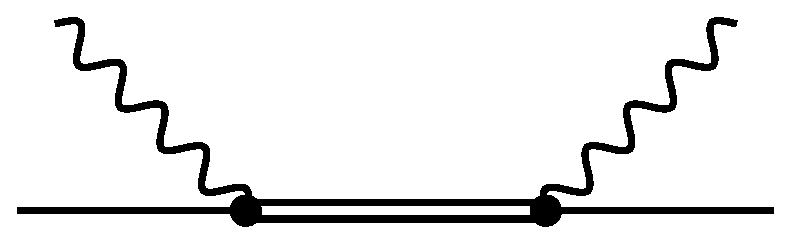
\epsfig{file=DeltaExchange.eps,width=6cm,angle=0}
\caption{$\Delta$-exchange diagram. \label{DeltaExchange}}
\end{figure}
In this section, we give analytical expressions for the contributions of the tree-level $\Delta$-exchange, cf.\ Fig.~\ref{DeltaExchange}, to the nucleon polarizabilities and their slopes at $Q^2=0$. Note that the $\Delta$-exchange equally contributions to proton and neutron polarizabilities. The $\gamma^* N \Delta$ vertex follows from the Lagrangian given in \Eqref{gammaNDeltaLag}:
\bea
%\Gamma_{\Delta \rightarrow \gamma N}^{\al \mu}&=&-\sqrt{\frac{3}{2}}\frac{e}{M(M+M_\Delta)}\left\{g_M \gamma^{\al \mu \kappa \lambda}p'_\kappa q_\lambda+g_E(p'\cdot q\, g^{\al \mu}-q^\al p^{\prime\mu})\right.\\
%&&\left.-\frac{g_C}{M_\Delta} \left(q^2 g^{ \al \mu}\slashed{p}'-q^2 p^{\prime\mu} \gamma^\al +p'\cdot q \,q^\mu \gamma^\al-q^\al q^\mu \slashed{p}'\right)\right\}\gamma_5,\qquad\nn\\
\Gamma_{\gamma N \rightarrow \Delta}^{\al \mu}&=&\sqrt{\frac{3}{2}}\frac{e}{M_N(M_N+M_\Delta)}\left\{g_M \gamma^{\al \mu \kappa \lambda}p'_\kappa q_\lambda+g_E (p'\cdot q\, g^{\al \mu}-q^\al p^{\prime\mu})\right.\\
&&\left.+\frac{g_C}{M_\Delta} \left(q^2 g^{ \al \mu}\slashed{p}'-q^2 p^{\prime\mu} \gamma^\al +p'\cdot q \,q^\mu \gamma^\al-q^\al q^\mu \slashed{p}'\right)\right\}\gamma_5,\qquad\nn
\eea
with $p+q=p'$, where $p$, $q$ and $p'$ are the momenta of nucleon, photon and delta, respectively. Here, we use $\delta = M_\Delta - M_N$, $M_+=M_\Delta+M_N$, and the couplings are given in Table \ref{tab:constants}.  Remember that for the magnetic coupling, we introduced the following $Q^2$ dependence: $g_M \rightarrow g_M/(1+Q^2/\Lambda^2)^2$.


\bea
\eqlab{alphabetaQ2}
\al_{E1}&=&-\frac{e^2 g_E^2}{2 \pi  M_+^3}\\
\be_{M1}&=&\frac{e^2 g_M^2}{2 \pi  \delta  M_+^2}\\
\al_L&=&\frac{e^2 M_\Delta^2}{\pi M_+^3}\left(\frac{ g_E^2}{\delta  M_NM_+^2}-\frac{g_C^2}{2 M_\Delta^4}+\frac{ g_E g_C}{M_NM_\Delta^2 M_+}\right)\\
\gamma_0&=&-\frac{e^2}{4\pi M_+^2}\left(\frac{g_M^2}{\delta^2}+\frac{g_E^2}{M_+^2}-\frac{4g_M g_E}{M_+\delta}\right)\\
\delta_{LT}&=&\frac{e^2 M_\Delta}{4\pi M_+^3}\left(\frac{g_E^2 }{M_N M_+}+\frac{g_M g_E }{\delta M_N}-\frac{g_E g_C}{M_\Delta^2}\right)\\
I_A&=&0\eqlab{IAstatic}\\
I_1&=&0\eqlab{I1static}\\
\bar d_2&=&0
\eea

\bea
\frac{\dd \left[\alpha_{E1}(Q^2)+\beta_{M1}(Q^2)\right]}{\dd Q^2}\Bigg\vert_{Q^2=0}&=&-\frac{e^2}{\pi M_+^2}\left(\frac{g_M^2}{\delta^2}\left[\frac{1}{M_+}-\frac{1}{2\delta}\right]+\frac{2}{ \Lambda^2 }\frac{g_M^2}{\delta}\right.+\frac{g_M g_E}{M_N}\left[\frac{1}{4\delta^2}-\frac{1}{\delta M_+}+\frac{1}{4M_+^2}\right]\nn\\
&&\left.-\frac{g_E^2}{4M_NM_+}\left[\frac{1}{\delta}-\frac{5}{M_+}\right]-\frac{ g_M g_C}{2  \delta  M_NM_+}+\frac{g_E g_C}{M_NM_+^2}\right)\qquad\\
\frac{\dd\, \al_L(Q^2)}{\dd Q^2}\Bigg\vert_{Q^2=0}&=&\frac{e^2 M_\Delta^3}{\pi \delta M_+^4}\left(\frac{2g_E^2}{\delta^2 M_+^2}\left[\frac{2}{M_\Delta}-\frac{1}{M_N}\right]-\frac{g_C^2}{ M_\Delta^4}\left[\frac{1}{M_N}-\frac{3}{2M_\Delta}\right]+\frac{g_E g_C}{\delta M_\Delta^2 M_+}\left[\frac{5}{M_\Delta}-\frac{3}{M_N}\right]\right)\qquad\\
\frac{\dd \gamma_0(Q^2)}{\dd Q^2}\Bigg\vert_{Q^2=0}&=&-\frac{e^2}{\pi M_+^2 \delta}\left(\frac{g_M^2}{\delta}\left[\frac{1}{4\delta^2}-\frac{1}{\delta M_+}+\frac{1}{2 M_+^2}\right]-\frac{1}{\Lambda^2}\frac{g_M^2}{ \delta}+\frac{g_E^2}{2 M_+^2}\left[\frac{1}{2\delta}-\frac{3}{M_+}\right]\right.\nn\\
&& \left.-\frac{g_M g_E}{M_+}\left[\frac{1}{\delta^2}-\frac{5}{\delta M_+}+\frac{1}{M_+^2}\right]+\frac{1}{\Lambda^2}\frac{2g_M g_E}{ M_+}+\frac{2 g_M g_C}{\delta M_+^2}-\frac{g_E g_C}{M_+^3}\right)\\
\frac{\dd\, \delta_{LT}(Q^2)}{\dd Q^2}\Bigg\vert_{Q^2=0}&=&\frac{e^2  M_\Delta \delta}{4
\pi M_NM_+^2}\left(\frac{g_E^2 }{\delta^2 M_+^2}\left[\frac{1}{\delta}-\frac{4}{M_+}\right]-\frac{g_C^2}{\delta M_\Delta^2 M_+^2}+\frac{g_M g_E }{\delta^2 M_+}\left[\frac{1}{\delta^2}-\frac{3}{\delta M_+}+\frac{1}{M_+^2}\right]\right.\nn\\
&&\left.-\frac{2}{ \Lambda^2}\frac{g_M g_E }{\delta^2M_+}+\frac{g_M g_C}{\delta M_\Delta^2 }\left[\frac{1}{2\delta^2}-\frac{2}{\delta M_+}+\frac{1}{2 M_+^2}\right]-\frac{g_E g_C}{2M_\Delta^2 M_+^2}\left[\frac{7}{\delta}+\frac{1}{M_+}\right]\right)\\
\frac{\dd\, I_A(Q^2)}{\dd Q^2}\Bigg\vert_{Q^2=0}&=&-\frac{M_N^2}{M_+^2}\left(\frac{g_M^2}{2 \delta ^2}+\frac{g_E^2}{M_NM_+}-\frac{2 g_M g_E}{\delta  M_+}-\frac{g_E g_C}{M_\Delta M_+}\right)\\
\frac{\dd\, I_1(Q^2)}{\dd Q^2}\Bigg\vert_{Q^2=0}&=&-\frac{M_\Delta M_N^2}{2M_+^3}\left(\frac{g_E^2}{M_N M_\Delta}-\frac{g_M g_E}{ \delta  M_N}
-\frac{g_E g_C}{M_\Delta^2 }\right)\\
\eqlab{d2momQ2}
\frac{\dd\, \bar d_2(Q^2)}{\dd Q^2}\Bigg\vert_{Q^2=0}&=&0
\eea



\beq
\frac{1}{6}\frac{\dd^3\, \bar d_2(Q^2)}{\dd( Q^2)^3}\Bigg\vert_{\substack{Q^2=0\\ \Lambda \rightarrow \infty}}=\frac{M_\Delta}{16M_N^2M_+^2}\left(\frac{g_M^2}{ \delta ^2 M_\Delta}+\frac{g_E^2}{M_+^2}\left[\frac{3 }{ M_N}+\frac{1}{M_\Delta}\right]+\frac{g_M g_E}{\Delta M_+ }\left[\frac{3}{ M_N}-\frac{4}{M_\Delta}\right]-\frac{3 g_E g_C}{ M_\Delta^2 M_+}\right)
\eeq





\end{widetext}



\section*{Acknowledgements}

We thank Lothar Tiator and Marc Vanderhaeghen for helpful discussions. This work is supported by the Deutsche Forschungsgemeinschaft (DFG) through the
Collaborative Research Center [The Low-Energy Frontier of the Standard Model (SFB 1044)]. Furthermore, the work of 
J.M.A.\ is partially funded by DFG and NSFC through the Sino-German CRC 110 [Symmetries and the Emergence of Structure in QCD (NSFC Grant No. 11261130311)] and by the MINECO (Spain) and ERDF (European Commission) grant FPA2013-40483-P. The work of F.H.\ is partially funded by the Swiss National Science Foundation.

\begin{thebibliography}{99} 

\bibitem{Pohl:2010zza} 
  R.~Pohl, A.~Antognini, F.~Nez, F.~D.~Amaro, F.~Biraben, J.~M.~R.~Cardoso, D.~S.~Covita and A.~Dax {\it et al.},
  %``The size of the proton,''
  Nature {\bf 466}, 213 (2010).
  %%CITATION = NATUA,466,213;%%
  
\bibitem{Antognini:1900ns}
A.~Antognini, {\it et al.}\, Science {\bf 339}, 417-420 (2013).
%Proton Structure from the Measurement of $2S-2P$ Transition Frequencies of Muonic Hydrogen",
%%CITATION = SCIEA,339,417;%%"

  
  %\cite{Pohl:2013yb}
\bibitem{Pohl:2013yb} 
  R.~Pohl, R.~Gilman, G.~A.~Miller and K.~Pachucki,
  %``Muonic hydrogen and the proton radius puzzle,''
Ann.\ Rev.\ Nucl.\ Part.\ Sci.\ {\bf 63} (2013) 175-204.
  %%CITATION = ARXIV:1301.0905;%%
  
  \bibitem{Hagelstein:2015egb} 
  F.~Hagelstein, R.~Miskimen and V.~Pascalutsa,
  %``Nucleon Polarizabilities: from Compton Scattering to Hydrogen Atom,''
  Prog.\ Part.\ Nucl.\ Phys.\  {\bf 88}, 29 (2016). 
 % doi:10.1016/j.ppnp.2015.12.001
 % [arXiv:1512.03765 [nucl-th]].
  %%CITATION = doi:10.1016/j.ppnp.2015.12.001;%%
  
\bibitem{Bernard:2012hb} 
  V.~Bernard, E.~Epelbaum, H.~Krebs and U.-G.~Mei\ss ner,
  %``New insights into the spin structure of the nucleon,''
  Phys.\ Rev.\ D {\bf 87}, 054032 (2013).
 % [arXiv:1209.2523 [hep-ph]].
  %%CITATION = ARXIV:1209.2523;%%
  
   
  %\cite{Birse:2012eb}
\bibitem{Birse:2012eb} 
  M.~C.~Birse and J.~A.~McGovern,
  %``Proton polarisability contribution to the Lamb shift in muonic hydrogen at fourth order in chiral perturbation theory,''
  Eur.\ Phys.\ J.\ A {\bf 48}, 120 (2012).
 % [arXiv:1206.3030 [hep-ph]].
  %%CITATION = ARXIV:1206.3030;%%
  
  \bibitem{Kao:2002cp} 
  C.~W.~Kao, T.~Spitzenberg and M.~Vanderhaeghen,
  %``Burkhardt-Cottingham sum rule and forward spin polarizabilities in heavy baryon chiral perturbation theory,''
  Phys.\ Rev.\ D {\bf 67}, 016001 (2003).
 % [hep-ph/0209241].
  %%CITATION = HEP-PH/0209241;%%
  
    \bibitem{Bernauer:2010wm} 
  J.~C.~Bernauer {\it et al.}  [A1 Collaboration],
  %``High-precision determination of the electric and magnetic form factors of the proton,''
  Phys.\ Rev.\ Lett.\  {\bf 105}, 242001 (2010)
  [arXiv:1007.5076 [nucl-ex]].
  %%CITATION = ARXIV:1007.5076;%%
  
  \bibitem{Mohr:2015ccw}
P.~J.~Mohr, D.~B.~Newell and B.~N.~Taylor, Rev.\ Mod.\ Phys.\ {\bf 88}, 035009 (2016).
%CODATA Recommended Values of the Fundamental Physical Constants: 2014}
%%CITATION = ARXIV:1507.07956;%%"
  
\bibitem{Pohl:2016xsr}
R.~Pohl, et al., arXiv: 1609.03440 [physics.atom-ph] (2016).
%"Laser Spectroscopy of Muonic Atoms and Ions}",
%"{12th International Conference on Low Energy Antiproton Physics (LEAP2016) Kanazawa, Japan, March 6-11, 2016}",
%%CITATION = ARXIV:1609.03440;%%"

  
  \bibitem{Drechsel:2002ar} 
  D.~Drechsel, B.~Pasquini and M.~Vanderhaeghen,
  %``Dispersion relations in real and virtual Compton scattering,''
  Phys.\ Rept.\  {\bf 378}, 99 (2003)
  [hep-ph/0212124].
  %%CITATION = HEP-PH/0212124;%%
  
      \bibitem{BaldinSumRule} 
  A.~M.~Baldin, Nucl. Phys. B {\bf 18}, 310 (1960),
  
  \bibitem{Gerasimov:1965et} 
  S.~B.~Gerasimov,
  %``A Sum rule for magnetic moments and the damping of the nucleon magnetic moment in nuclei,''
  Sov.\ J.\ Nucl.\ Phys.\  {\bf 2}, 430 (1966)
  [Yad.\ Fiz.\  {\bf 2}, 598 (1965)].
  %%CITATION = SJNCA,2,430;%%
  
  \bibitem{Drell:1966jv} 
  S.~D.~Drell and A.~C.~Hearn,
  %``Exact Sum Rule for Nucleon Magnetic Moments,''
  Phys.\ Rev.\ Lett.\  {\bf 16}, 908 (1966).
  %%CITATION = PRLTA,16,908;%%
  
 
  \bibitem{Ahrens:2001qt} 
  J.~Ahrens {\it et al.}  [GDH and A2 Collaborations],
  %``First measurement of the Gerasimov-Drell-Hearn integral for Hydrogen from 200 to 800 MeV,''
  Phys.\ Rev.\ Lett.\  {\bf 87}, 022003 (2001)
  [hep-ex/0105089].
  %%CITATION = HEP-EX/0105089;%%
  
  \bibitem{Helbing:2002eg} 
  K.~Helbing [GDH Collaboration],
  %``Experimental verification of the GDH sum rule at ELSA and MAMI,''
  Nucl.\ Phys.\ Proc.\ Suppl.\  {\bf 105}, 113 (2002).
  %%CITATION = NUPHZ,105,113;%%
  
  \bibitem{Alarcon:2013cba} 
  J.~M.~Alarcon, V.~Lensky and V.~Pascalutsa,
  %``Chiral perturbation theory of muonic hydrogen Lamb shift: polarizability contribution,''
  Eur.\ Phys.\ J.\ C {\bf 74}, 2852 (2014)
  [arXiv:1312.1219 [hep-ph]].
  %%CITATION = ARXIV:1312.1219;%%
  
  \bibitem{LET}
F.~E.~Low,
  %``Scattering of light of very low frequency by systems of spin 1/2,''
  Phys.\ Rev.\  {\bf 96}, 1428 (1954); 
     %%CITATION = PHRVA,96,1428;%%
  M.~Gell-Mann and M.~L.~Goldberger,
  %``Scattering of low-energy photons by particles of spin 1/2,''
  Phys.\ Rev.\  {\bf 96}, 1433 (1954).
 %%CITATION = PHRVA,96,1433;%%
  
 \bibitem{Amarian:2004yf} 
  M.~Amarian {\it et al.}  [Jefferson Lab E94010 Collaboration],
  %``Measurement of the generalized forward spin polarizabilities of the neutron,''
  Phys.\ Rev.\ Lett.\  {\bf 93}, 152301 (2004).
%  [nucl-ex/0406005].
  %%CITATION = NUCL-EX/0406005;%%



  
  
  \bibitem{Bernard:1991rq} 
  V.~Bernard, N.~Kaiser and U.-G.~Mei\ss ner,
  %``Chiral expansion of the nucleon's electromagnetic polarizabilities,''
  Phys.\ Rev.\ Lett.\  {\bf 67}, 1515 (1991).
  %%CITATION = PRLTA,67,1515;%%



\bibitem{Wandzura:1977qf} 
  S.~Wandzura and F.~Wilczek,
  %``Sum Rules for Spin Dependent Electroproduction: Test of Relativistic Constituent Quarks,''
  Phys.\ Lett.\ B {\bf 72}, 195 (1977).
  %%CITATION = PHLTA,B72,195;%%




\bibitem{Drechsel:1992pn} 
  D.~Drechsel and L.~Tiator,
  %``Threshold pion photoproduction on nucleons,''
  J.\ Phys.\ G {\bf 18}, 449 (1992)

\bibitem{Drechsel:2000ct} 
  D.~Drechsel, S.~S.~Kamalov and L.~Tiator,
  %``The GDH sum rule and related integrals,''
  Phys.\ Rev.\ D {\bf 63}, 114010 (2001)
  [hep-ph/0008306].
  %%CITATION = HEP-PH/0008306;%%
  
 \bibitem{Drechsel:1998hk} 
  D.~Drechsel, O.~Hanstein, S.~S.~Kamalov, L.~Tiator and ,
  %``A Unitary isobar model for pion photoproduction and electroproduction on the proton up to 1-GeV,''
  Nucl.\ Phys.\ A {\bf 645}, 145 (1999)
  [nucl-th/9807001].
  %%CITATION = NUCL-TH/9807001;%%

\bibitem{Babusci:1997ij} 
  D.~Babusci, G.~Giordano and G.~Matone,
  %``A New evaluation of the Baldin sum rule,''
  Phys.\ Rev.\ C {\bf 57}, 291 (1998)
  [nucl-th/9710017].
  %%CITATION = NUCL-TH/9710017;%%
  
  \bibitem{Liang:2004tk} 
  Y.~Liang, M.~E.~Christy, R.~Ent and C.~E.~Keppel,
  %``Q**2 evolution of generalized Baldin sum rule for the proton,''
  Phys.\ Rev.\ C {\bf 73}, 065201 (2006)
  [nucl-ex/0410028].
  %%CITATION = NUCL-EX/0410028;%%

\bibitem{Lensky:2009uv} 
  V.~Lensky and V.~Pascalutsa
  %``Predictive powers of chiral perturbation theory in Compton scattering off protons,''
  Eur.\ Phys.\ J.\ C {\bf 65}, 195 (2010)
  [arXiv:0907.0451 [hep-ph]].
  %%CITATION = ARXIV:0907.0451;%%

 \bibitem{Pascalutsa:2002pi} 
 V.~Pascalutsa and D.~R.~Phillips,
    %``Effective theory of the Delta(1232) in Compton scattering off the
  %nucleon,''
  Phys.\ Rev.\  C {\bf 67}, 055202 (2003).
  %[arXiv:nucl-th/0212024].
  %%CITATION = PHRVA,C67,055202;%%



\bibitem{Bernard:1995dp} 
  V.~Bernard, N.~Kaiser, U.-G.~Mei\ss ner,
  %``Chiral dynamics in nucleons and nuclei,''
  Int.\ J.\ Mod.\ Phys.\ E {\bf 4}, 193 (1995)
  [hep-ph/9501384].
  %%CITATION = HEP-PH/9501384;%%

\bibitem{Prok:2008ev} 
 Y.~Prok {\it et al.}  [CLAS Collaboration],
  %``Moments of the Spin Structure Functions g**p(1) and g**d(1) for 0.05 < Q**2 < 3.0-GeV**2,''
  Phys.\ Lett.\ B {\bf 672}, 12 (2009)
  [arXiv:0802.2232 [nucl-ex]].
  %%CITATION = ARXIV:0802.2232;%%

\bibitem{Dutz:2003mm} 
  H.~Dutz {\it et al.}  [GDH Collaboration],
  %``First measurement of the Gerasimov-Drell-Hearn sum rule for H-1 from 0.7-GeV to 1.8-GeV at ELSA,''
  Phys.\ Rev.\ Lett.\  {\bf 91}, 192001 (2003).
  %%CITATION = PRLTA,91,192001;%%

\bibitem{Amarian:2004yf} 
  M.~Amarian {\it et al.}  [Jefferson Lab E94010 Collaboration],
  %``Measurement of the generalized forward spin polarizabilities of the neutron,''
  Phys.\ Rev.\ Lett.\  {\bf 93}, 152301 (2004)
  [nucl-ex/0406005].
  %%CITATION = NUCL-EX/0406005;%%


\bibitem{Kochelev:2011bh} 
  N.~Kochelev and Y.~Oh,
  %``Axial anomaly and the $\delta_{LT}$ puzzle,''
  Phys.\ Rev.\ D {\bf 85}, 016012 (2012)
  [hep-ph/1103.4892].
  %%CITATION = ARXIV:1103.4892;%%



\bibitem{Hand:1963bb} 
  L.~N.~Hand,
  %``Experimental investigation of pion electroproduction,''
  Phys.\ Rev.\  {\bf 129}, 1834 (1963).
  %%CITATION = PHRVA,129,1834;%%

\bibitem{Gilman:1967sn} 
  F.~J.~Gilman,
  %``The Kinematics And Saturation Of The Sum Rules And Inequalities For Inelastic Electron Scattering,''
  Phys.\ Rev.\  {\bf 167}, 1365 (1968).
  %%CITATION = PHRVA,167,1365;%%
  
\bibitem{Holstein:2005db} 
  B.~R.~Holstein, V.~Pascalutsa and M.~Vanderhaeghen,
  %``Sum rules for magnetic moments and polarizabilities in QED and chiral effective-field theory,''
  Phys.\ Rev.\ D {\bf 72}, 094014 (2005)
  [hep-ph/0507016].
  %%CITATION = HEP-PH/0507016;%%
  
  \bibitem{Pasquini:2007fw} 
  B.~Pasquini, D.~Drechsel and L.~Tiator,
  %``Invariant amplitudes for pion electroproduction,''
  Eur.\ Phys.\ J.\ A {\bf 34}, 387 (2007)
  [hep-ph/0712.2327].
  
  \bibitem{Sibirtsev:2013cga} 
  A.~Sibirtsev and P.~G.~Blunden,
  %``Q^2-evolution of the electric and magnetic polarizabilities of the proton,''
Phys.\ Rev.\ C {\bf 88}, 065202 (2013) [nucl-th/1311.6482].
%%CITATION = ARXIV:1311.6482;%%"



  \bibitem{Bernard:2002pw} 
  V.~Bernard, T.~R.~Hemmert and U.-G.~Mei\ss ner,
  %``Spin structure of the nucleon at low-energies,''
  Phys.\ Rev.\ D {\bf 67}, 076008 (2003)
  [hep-ph/0212033].
  %%CITATION = HEP-PH/0212033;%%

\bibitem{Bernard:2002bs}
V.~Bernard, T.~R.~Hemmert, and U.~Mei\ss ner,
%Novel analysis of chiral loop effects in the generalized Gerasimov-Drell-Hearn sum rule}
Phys.\ Lett.\ B {\bf 545}, 105-111 (2002).
%%CITATION = HEP-PH/0203167;%%"


\bibitem{Alarcon:2012kn} 
  J.~M.~Alarc\'on, J.~Martin Camalich and J.~A.~Oller,
  %``Improved description of the $\pi N$-scattering phenomenology in covariant baryon chiral perturbation theory,''
    Phys.\ Rev.\ D {\bf 85}, 051503 (2012);  Annals Phys.\  {\bf 336}, 413 (2013).
  %%CITATION = ARXIV:1210.4450;%%
  %%CITATION = ARXIV:1110.3797;%%
  
  
  \bibitem{Chen:2012nx} 
  Y.~-H.~Chen, D.~-L.~Yao and H.~Q.~Zheng,
  %``Analyses of pion-nucleon elastic scattering amplitudes up to $O(p^4)$ in extended-on-mass-shell subtraction scheme,''
  Phys.\ Rev.\ D {\bf 87}, no. 5, 054019 (2013).
  %%CITATION = ARXIV:1212.1893;%%

\bibitem{Siemens:2014pma} 
  D.~Siemens, V.~Bernard, E.~Epelbaum, H.~Krebs and U.-G.~Mei\ss ner,
  %``The reaction pi N -> pi pi N in chiral effective field theory with explicit Delta(1232) degrees of freedom,''
 Phys.\ Rev.\ C {\bf 89}, 065211 (2014) [nucl-th/1403.2510].
%%CITATION = ARXIV:1403.2510;%%"

  
  
  \bibitem{Pascalutsa:2005vq} 
  V.~Pascalutsa and M.~Vanderhaeghen,
  %``Chiral effective-field theory in the Delta(1232) region: I. Pion electroproduction on the nucleon,''
  Phys.\ Rev.\ D {\bf 73}, 034003 (2006)
  [hep-ph/0512244].
  %%CITATION = HEP-PH/0512244;%%
  
  
  \bibitem{Pascalutsa:2006up}
  V.~Pascalutsa, M.~Vanderhaeghen and S.~N.~Yang,
   Phys.\ Rept.\ {\bf 437}, 125-232 (2007)
   [hep-ph/0609004].
  
  \bibitem{Hall:2014lea} 
  N.~L.~Hall, A.~W.~Thomas and R.~D.~Young,
  %``Momentum transfer dependence of the proton's electric and magnetic polarizabilities,''
Phys.\ Rev.\ D {\bf 89}, 117502 (2014)  [nucl-th/1401.8062].
%%CITATION = ARXIV:1401.8062;%%"

  
  \bibitem{Carlson:2008ke} 
  C.~E.~Carlson, V.~Nazaryan and K.~Griffioen,
  %``Proton structure corrections to electronic and muonic hydrogen hyperfine splitting,''
  Phys.\ Rev.\ A {\bf 78}, 022517 (2008)
  [physics.atom-ph/0805.2603.
  %%CITATION = ARXIV:0805.2603;%%

 \bibitem{private-Lothar}
L. Tiator, private communication.

\bibitem{Hagelstein:2015lph}
F.~Hagelstein and V.~Pascalutsa, PoS, {\bf CD15}, 077 (2016) [nucl-th/1511.04301].

%Proton structure in the hyperfine splitting of muonic
%%CITATION = ARXIV:1511.04301;%%"

\bibitem{Hagelstein:2017cbl}
F.~Hagelstein, PhD thesis (2017) [nucl-th/1710.00874].
%%CITATION = ARXIV:1710.00874;%%"


\bibitem{Bernard:1991rq} 
  V.~Bernard, N.~Kaiser and U.~G.~Meissner,
  %``Chiral expansion of the nucleon's electromagnetic polarizabilities,''
  Phys.\ Rev.\ Lett.\  {\bf 67}, 1515 (1991).
  %%CITATION = PRLTA,67,1515;%%

\bibitem{Bernard:1991ru} 
  V.~Bernard, N.~Kaiser and U.~G.~Meissner,
  %``Nucleons with chiral loops: Electromagnetic polarizabilities,''
  Nucl.\ Phys.\ B {\bf 373}, 346 (1992).
  %%CITATION = NUPHA,B373,346;%%
  
  \bibitem{Kao:2003jd} 
  C.~-W.~Kao, D.~Drechsel, S.~Kamalov and M.~Vanderhaeghen,
  %``Higher moments of nucleon spin structure functions in heavy baryon chiral perturbation theory and in a resonance model,''
  Phys.\ Rev.\ D {\bf 69}, 056004 (2004)
  [hep-ph/0312102].
  %%CITATION = HEP-PH/0312102;%%

\bibitem{Carlson:2011zd} 
  C.~E.~Carlson and M.~Vanderhaeghen,
  %``Higher order proton structure corrections to the Lamb shift in muonic hydrogen,''
  Phys.\ Rev.\ A {\bf 84}, 020102 (2011)
  [hep-ph/1101.5965].
  %%CITATION = ARXIV:1101.5965;%%
  
  \bibitem{Nevado:2007dd} 
  D.~Nevado and A.~Pineda,
  %``Forward virtual Compton scattering and the Lamb shift in chiral perturbation theory,''
  Phys.\ Rev.\ C {\bf 77}, 035202 (2008)
  [hep-ph/0712.1294].
  %%CITATION = ARXIV:0712.1294;%%
  
  \bibitem{Peset:2014yha} 
  C.~Peset and A.~Pineda,
  %``Model independent determination of the muonic hydrogen Lamb shift and proton radius,''
Eur.\ Phys.\ J.\ A {\bf 51}, 32 (2015)  [hep-ph/1403.3408].
 %%CITATION = ARXIV:1403.3408;%%"

  
  \bibitem{Hemmert:1996rw} 
  T.~R.~Hemmert, B.~R.~Holstein and J.~Kambor,
  %``Delta (1232) and the polarizabilities of the nucleon,''
  Phys.\ Rev.\ D {\bf 55}, 5598 (1997)
  [hep-ph/9612374].
  %%CITATION = HEP-PH/9612374;%%

\bibitem {OlmosdeLeon:2001zn}
V.~Olmos de Leon, F.~Wissmann, P.~Achenbach, J.~Ahrens, H.~J.~Arends, R.~Beck, P.~D.~Harty and V.~Hejny {\it et al.}, 
% ``Low - energy Compton scattering and the polarizabilities of the proton, ''
Eur.\ Phys.\ J.\ A {\bf 10}, 207 (2001). 
%%CITATION = EPHJA, A10, 207; %%


\bibitem{Wandzura:1977qf} 
  S.~Wandzura and F.~Wilczek,
  %``Sum Rules for Spin Dependent Electroproduction: Test of Relativistic Constituent Quarks,''
  Phys.\ Lett.\ B {\bf 72}, 195 (1977).
  %%CITATION = PHLTA,B72,195;%%
  
  \bibitem{Amarian:2002ar} 
  M.~Amarian, L.~Auerbach, T.~Averett, J.~Berthot, P.~Bertin, W.~Bertozzi, T.~Black and E.~Brash {\it et al.},
  %``The Q**2 evolution of the generalized Gerasimov-Drell-Hearn integral for the neutron using a He-3 target,''
  Phys.\ Rev.\ Lett.\  {\bf 89}, 242301 (2002)
  [nucl-ex/0205020].
  %%CITATION = NUCL-EX/0205020;%%
  
  \bibitem{Exp-new-EG4}  
EG4 Collaboration. http://clasweb.jlab.org/gdh$\_$lowq2/

\bibitem{Exp-new-E08-027}
E08-027 Collaboration. http://hallaweb.jlab.org/experiment/E08-027/

\bibitem{Exp-new-E97-110}
E97-110 Collaboration. http://hallaweb.jlab.org/experiment/E97-110/

\bibitem{Bjorken:1966jh} 
  J.~D.~Bjorken,
  %``Applications of the Chiral U(6) x (6) Algebra of Current Densities,''
  Phys.\ Rev.\  {\bf 148}, 1467 (1966).
  %%CITATION = PHRVA,148,1467;%%
  
  \bibitem{Bjorken:1969mm} 
  J.~D.~Bjorken,
  %``Inelastic Scattering of Polarized Leptons from Polarized Nucleons,''
  Phys.\ Rev.\ D {\bf 1}, 1376 (1970).
  %%CITATION = PHRVA,D1,1376;%%
  
  \bibitem{Amarian:2003jy} 
  M.~Amarian {\it et al.}  [Jefferson Lab E94-010 Collaboration],
  %``Q**2 evolution of the neutron spin structure moments using a He-3 target,''
  Phys.\ Rev.\ Lett.\  {\bf 92}, 022301 (2004)
  [hep-ex/0310003].
  %%CITATION = HEP-EX/0310003;%%

\bibitem{Wandzura:1977qf} 
  S.~Wandzura and F.~Wilczek,
  %``Sum Rules for Spin Dependent Electroproduction: Test of Relativistic Constituent Quarks,''
  Phys.\ Lett.\ B {\bf 72}, 195 (1977).
  %%CITATION = PHLTA,B72,195;%%

\bibitem{Bradford:2006yz}
R.~Bradford, A.~Bodek, H.~S.~Budd and J.~Arrington, Nucl.\ Phys.\ Proc.\ Suppl.\ {\bf 159}, 127-132 (2006).
%A New parameterization of the nucleon elastic form-factors
%%CITATION = HEP-EX/0602017;%%"



%\bibitem{Drechsel:2007if} 
 % D.~Drechsel, S.~S.~Kamalov and L.~Tiator,
  %``Unitary Isobar Model - MAID2007,''
  %Eur.\ Phys.\ J.\ A {\bf 34}, 69 (2007).
  %[arXiv:0710.0306 [nucl-th]].
  %%CITATION = ARXIV:0710.0306;%%}
   
   \bibitem{Mohr:2012tt}
P.~J.~Mohr, B.~N.~Taylor and D.~B.~Newell,
%CODATA Recommended Values of the Fundamental Physical Constants: 2010
Rev.\ Mod.\ Phys.\ {\bf 84}, 1527-1605 (2012).
   
  \bibitem{GSS89}
J.~Gasser, M.~E.~Sainio and A.~Svarc,
%``Nucleons With Chiral Loops,''
Nucl.\ Phys.\ B {\bf 307}, 779 (1988).
%%CITATION = NUPHA,B307,779;%%

  %\cite{Lensky:2014dda}
\bibitem{Lensky:2014dda} 
  V.~Lensky, J.~M.~Alarc\'on and V.~Pascalutsa,
  %``Moments of nucleon structure functions at next-to-leading order in baryon chiral perturbation theory,''
  Phys.\ Rev.\ C {\bf 90}, no. 5, 055202 (2014)
  doi:10.1103/PhysRevC.90.055202
  [arXiv:1407.2574 [hep-ph]].
  %%CITATION = doi:10.1103/PhysRevC.90.055202;%%
  
  \bibitem{Pascalutsa:2005ts} 
  V.~Pascalutsa and M.~Vanderhaeghen,
  %``Electromagnetic nucleon-to-Delta transition in chiral effective-field theory,''
  Phys.\ Rev.\ Lett.\  {\bf 95}, 232001 (2005)
  [hep-ph/0508060].
  %%CITATION = HEP-PH/0508060;%%

\bibitem{Agashe:2014kda} 
  K.~A.~Olive {\it et al.}  [Particle Data Group Collaboration],
  %``Review of Particle Physics,''
  Chin.\ Phys.\ C {\bf 38}, 090001 (2014).
  %%CITATION = CHPHD,C38,090001;%%

\bibitem{Low:1954kd} 
  F.~E.~Low,
  %``Scattering of light of very low frequency by systems of spin 1/2,''
  Phys.\ Rev.\  {\bf 96}, 1428 (1954).
  %%CITATION = PHRVA,96,1428;%%

\bibitem{Guler:2015} 
N.~Guler, {\it et al.}, 
%Precise Determination of the Deuteron Spin Structure at Low to Moderate $Q^2$ with CLAS and Extraction of the Neutron Contribution
Phys.\ Rev.\ C {\bf 92}, 055201 (2015) [JLAB-PHY-15-2054; nucl-ex/1505.07877].
%%CITATION = ARXIV:1505.07877;%%"


\bibitem{MAID}
D.~Drechsel, S.~S.~Kamalov and L.~Tiator, Eur.\ Phys.\ J. A\ {\bf 34}, 69 (2007) 
[http://www.kph.uni-mainz.de/MAID/].

\bibitem{Deur:2008ej} 
  A.~Deur {\it et al.},
  %``Experimental study of isovector spin sum rules,''
  Phys.\ Rev.\ D {\bf 78}, 032001 (2008)
  [nucl-ex/0802.3198].
  %%CITATION = ARXIV:0802.3198;%%

\bibitem{Deur:2004ti} 
  A.~Deur {\it et al.},
  %``Experimental determination of the evolution of the Bjorken integral at low Q**2,''
  Phys.\ Rev.\ Lett.\  {\bf 93}, 212001 (2004)
  [hep-ex/0407007].
  %%CITATION = HEP-EX/0407007;%%

\bibitem{Gryniuk:2015} 
O.~Gryniuk, F.~Hagelstein and V.~Pascalutsa,
%Evaluation of the forward Compton scattering off protons: I. Spin-independent amplitude
Phys.\ Rev.\ D {\bf 92}, 074031 (2015). [nucl-th/1508.07952].
%%CITATION = ARXIV:1508.07952;%%"

\bibitem{Zielinski:2017gwp}
R.~Zielinski, PhD thesis (2017) [nucl-ex/1708.08297].
%"{The g2p Experiment: A Measurement of the Proton's Spin Structure Functions}",
%%CITATION = ARXIV:1708.08297;%%"

\end{thebibliography}



%%% FIGURES
 \begin{figure}[bt]
 \centering
 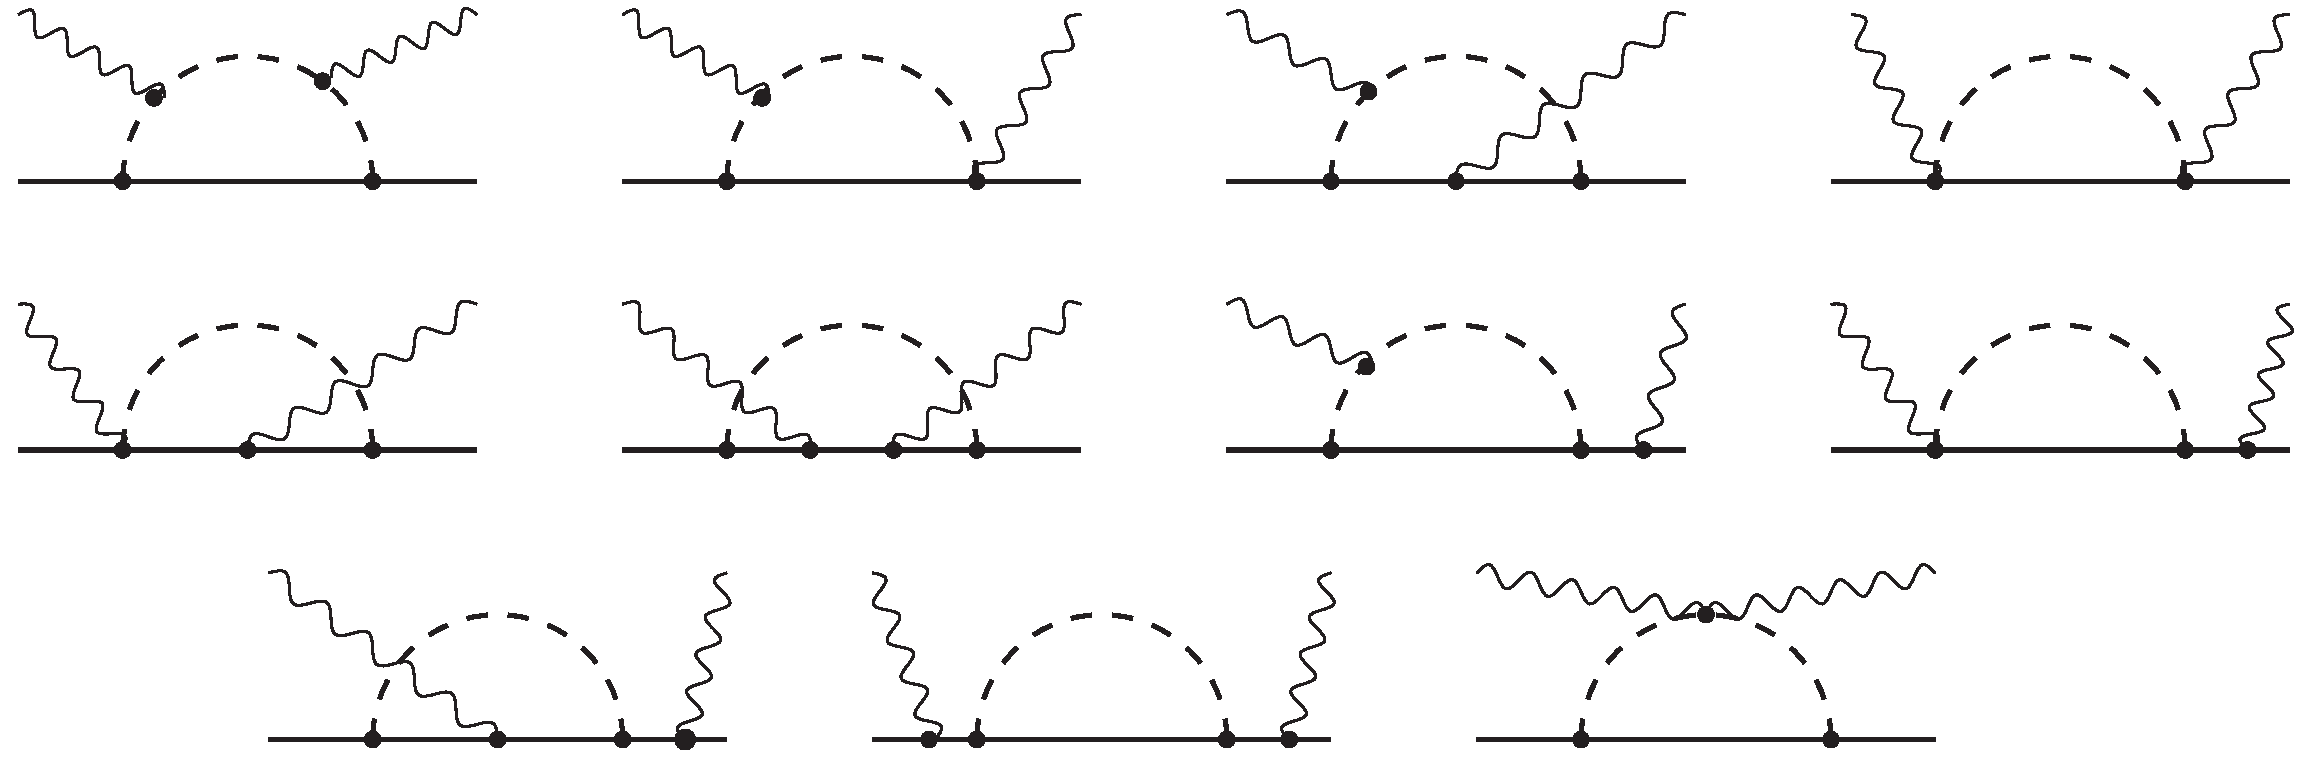
\includegraphics[width=0.95\columnwidth]{Diags1_pv.pdf} 
\caption{%(Color online)  
One-$\pi N$-loop graphs contributing to Compton scattering at $\mathcal{O}(p^3)$. Graphs obtained from these by
crossing and time-reversal are not shown, but are evaluated too.
}
\label{Fig:loops_pv}
\end{figure}

\begin{figure}[t]
\centering
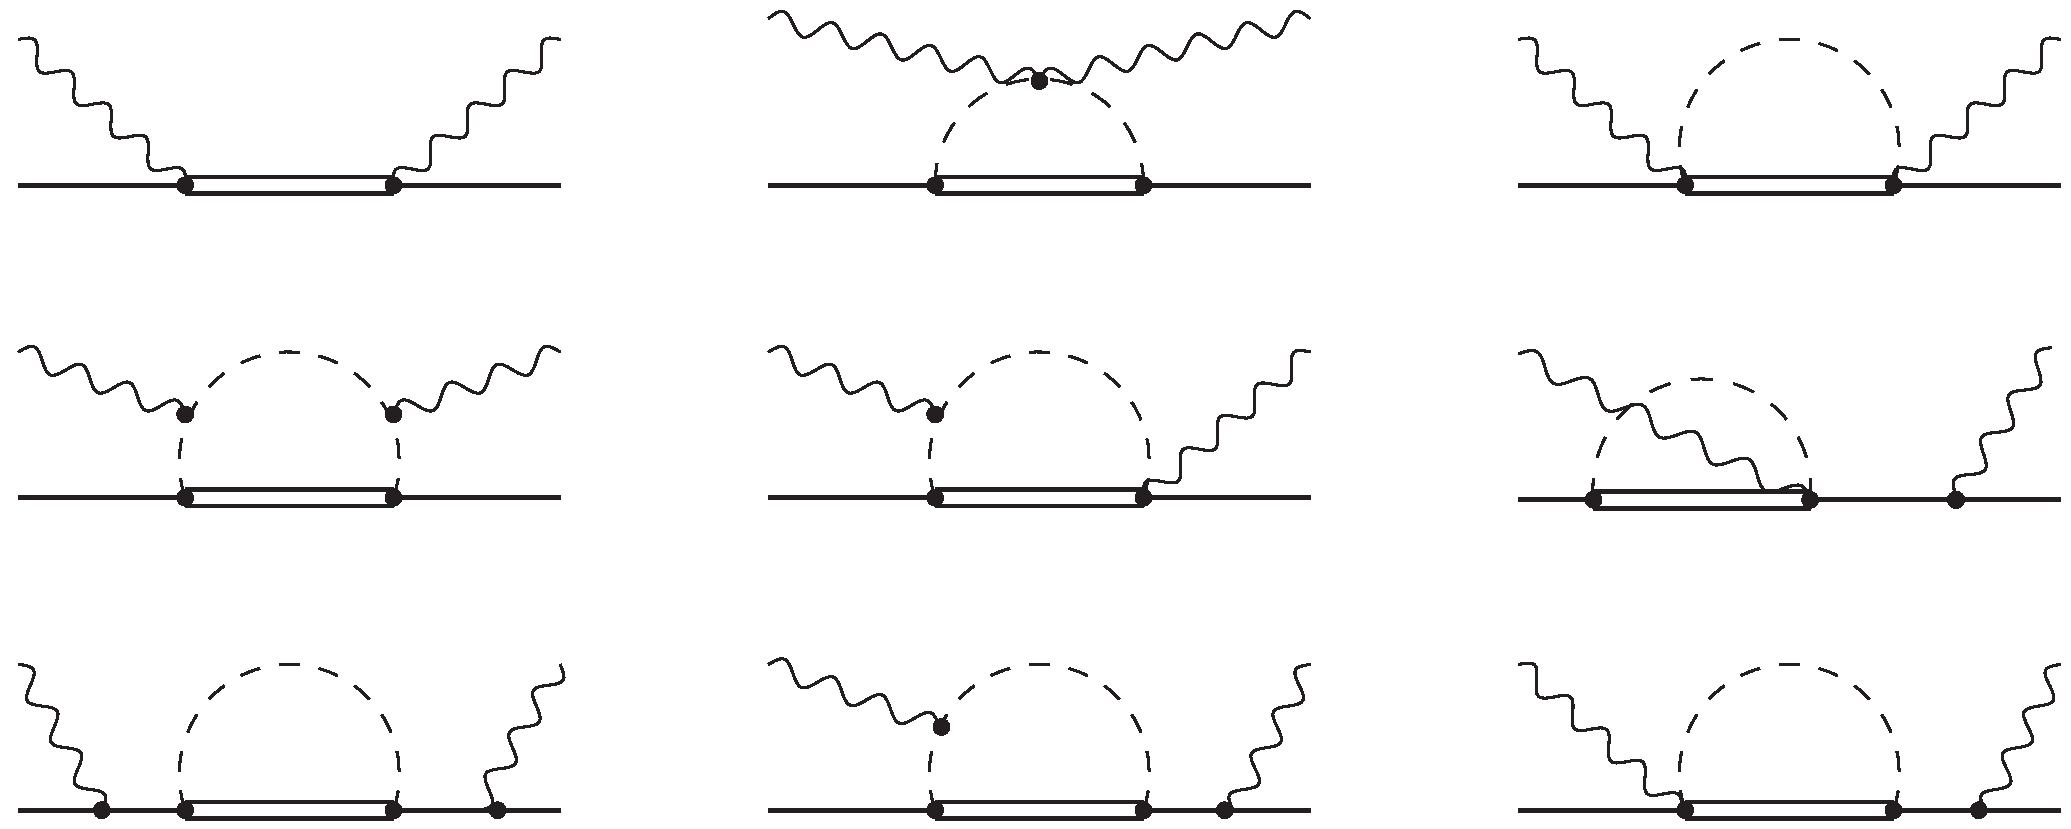
\includegraphics[width=0.95\columnwidth]{DeltaDiags4.pdf} 
\caption{%(Color online)  
Graphs contributing at  $\mathcal{O}(p^4/\mathit{\Delta})$. 
Double lines denote the propagator of the $\Delta$ isobar.
Graphs obtained from these by
crossing and time-reversal are evaluated too.}
\label{Fig:loopsD}
\end{figure}


\begin{figure*}
\begin{center}
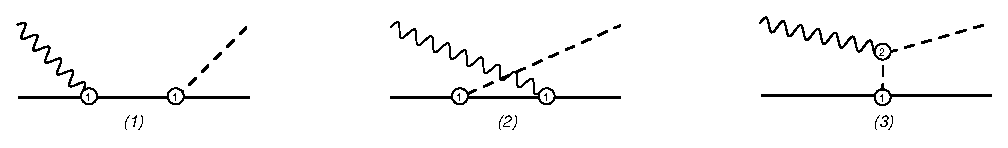
\epsfig{file=TreeLevelOp.eps,width=16cm,angle=0} 
\caption{Diagrams entering our calculation of the pion electroproduction amplitude at leading order. The numbers in the vertices indicate the chiral order of each one.\label{Fig:DiagsOp}}
\end{center}
\end{figure*}

\begin{figure}
\begin{center}
\epsfig{file=sigmaLT.pdf,width=8cm,angle=0} 
\caption{This figure illustrates the relation between the Compton and the photoabsorption part given by the optical theorem. In particular, we show the contributions to $\delta_{LT}(\nu,Q^2)$. The double-line arrows represent the spin of the external particles, while the dot represents the scalar (longitudinal) polarization of the incoming photon. Inside the blob the intermediate states are represented: nucleons with spins $r'$ (which are averaged in the calculation of the cross section) and pions. \label{Fig:sigmaLT}}
\end{center}
\end{figure}

\begin{figure}[H]
\begin{center}
\hspace{-0.3cm}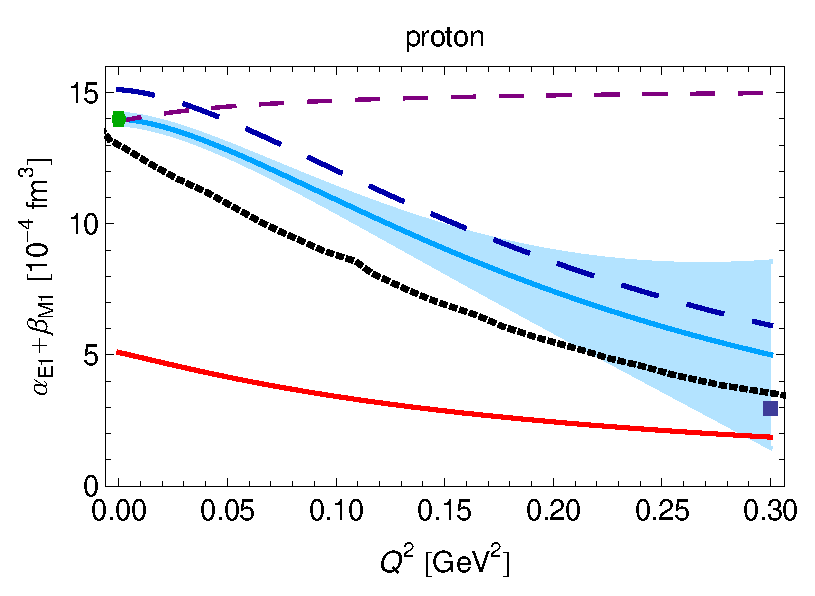
\epsfig{file=alpha+beta_p-Dip.eps,width=9cm,angle=0} \\[0.5cm]
\hspace{-0.3cm}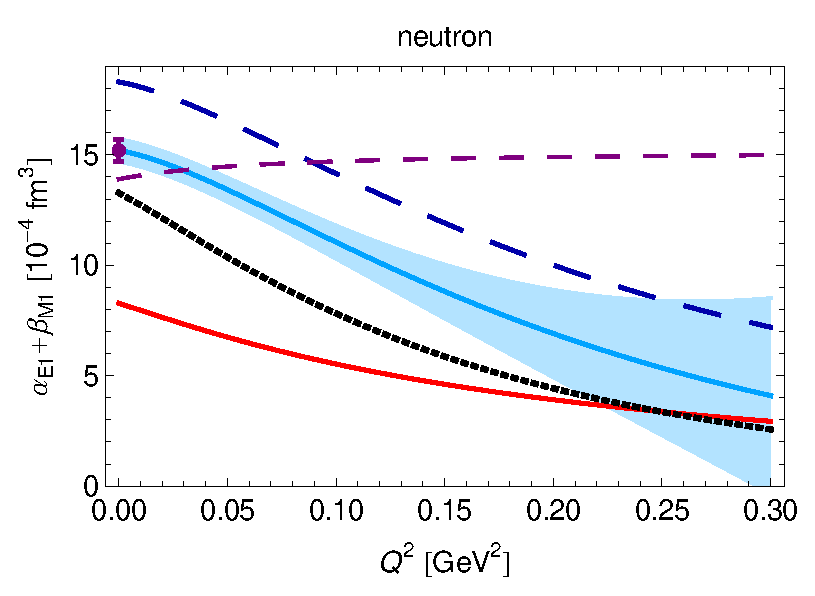
\epsfig{file=alpha+beta_n-Dip.eps,width=9cm,angle=0} 
\caption{Sum of electric and magnetic dipole polarizabilities, $\alpha_{E1}(Q^2)+\beta_{M1}(Q^2)$, for the proton ($p$) and neutron ($n$) as functions of $Q^2$.  
The result of this work is represented by the blue solid line and the blue band. The red line represents the $\pi$-cloud contribution in relativistic BChPT, while the blue short-dashed line is the LO HB limit \cite{Nevado:2007dd}.
The black dotted line represents the MAID estimate \cite{Drechsel:2000ct,Drechsel:1998hk} given in Ref.~\cite{Drechsel:2002ar} for the proton, using $\pi+\eta+\pi\pi$ channels. The green dot at $Q^2=0$ correspond to the Baldin sum rule evaluation for the proton reported in Ref.~\cite{Gryniuk:2015}. This value agrees well with other works \cite{OlmosdeLeon:2001zn, Babusci:1997ij} and therefore we refrain from indicating them in addition. For the neutron, the purple dot corresponds to the phenomenological extraction reported in Ref.~\cite{Babusci:1997ij}.
At finite momentum transfer, in the region considered, we have available the $Q^2=0.3$~GeV$^2$ point (blue dot) obtained in Ref.~\cite{Liang:2004tk} through evaluation of the generalized Baldin sum rule. \label{Fig:alpha+betaplot}}
\end{center}
\end{figure}

\begin{figure}[H]
\begin{center}
\hspace{-0.3cm}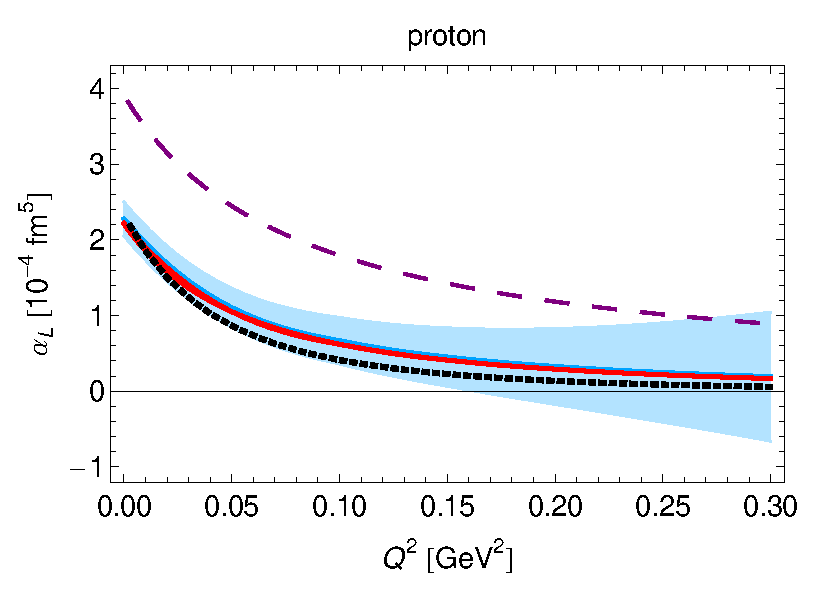
\epsfig{file=alphaL_p.eps,width=9cm,angle=0}\\[0.5cm]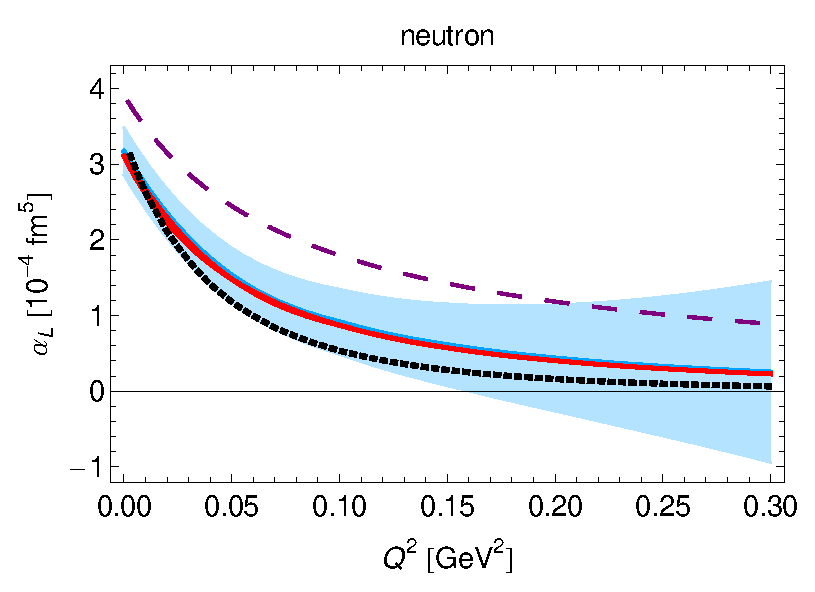
\epsfig{file=alphaL_n.eps,width=9cm,angle=0}
\caption{Longitudinal polarizabilities, $\alpha_L (Q^2)$, for the proton  (p) and neutron (n) as functions of $Q^2$. The legend is the same as in Fig.~\ref{Fig:alpha+betaplot} except for the black dotted line which correspond to the MAID estimate using only the $\pi$-channel, as in Ref.~\cite{Drechsel:2002ar}.  \label{Fig:alphaLplot}}
\end{center}
\end{figure}

\begin{figure}[H]
\begin{center}
\hspace{-0.3cm}\epsfig{file=gamma0_p-Dip.eps,width=9cm,angle=0}\\[0.5cm]
 \hspace{-0.3cm}\epsfig{file=gamma0_n-Dip.eps,width=9cm,angle=0}
\caption{Forward spin polarizabilities, $\gamma_0(Q^2)$, for the proton (p) and neutron (n) as functions of $Q^2$. 
For the blue band and the red line the legend is the same as in Fig.~\ref{Fig:alpha+betaplot}. The $\mathcal{O}(p^3)+\mathcal{O}(p^4)$ HB result of Ref.~\cite{Kao:2002cp} is indicated by the blue short-dashed line, however for the proton the prediction lies outside the range of values displayed in the figure. 
The MAID curves, both in black dotted lines, are from Ref.~\cite{Drechsel:2002ar} in the case of the proton, and Ref.~\cite{Amarian:2004yf} in the case of the neutron. 
The experimental determinations for the proton are taken from Ref.~\cite{Prok:2008ev} (blue dots), Ref.~\cite{Dutz:2003mm} (purple dot) and Ref.~\cite{Zielinski:2017gwp} (orange dot; uncertainties added in quadrature), while for the neutron the blue dots are from Ref.~\cite{Amarian:2004yf} and the green dots are from Ref.~\cite{Guler:2015} (statistical and systematic uncertainties added in quadrature). The pink band is the IR result of Ref.~\cite{Bernard:2002pw} and the gray band is the BChPT+$\Delta$ result of Ref.~\cite{Bernard:2012hb}. \label{Fig:gamma0plot}}
\end{center}
\end{figure}

\begin{figure}[H]
\begin{center}
\hspace{-0.3cm}\epsfig{file=deltaLT_p-Dip.eps,width=9cm,angle=0} \\[0.5cm]\hspace{-0.3cm}\epsfig{file=deltaLT_n-Dip.eps,width=9cm,angle=0} 
\caption{Longitudinal-transverse spin polarizabilities, $\delta_{LT}(Q^2)$, for the proton (p) and neutron (n) as functions of $Q^2$. 
For the blue band, the red line, and the black dotted line the legend is the same as in Fig.~\ref{Fig:alpha+betaplot}. 
The orange dot-dashed and blue short-dashed line are the $\mathcal{O}(p^3)$ and $\mathcal{O}(p^3)+\mathcal{O}(p^4)$ HB calculations of Ref.~\cite{Kao:2002cp}. The pink band is the IR result of Ref.~\cite{Bernard:2002pw} and the gray band is the covariant BChPT calculation including the $\Delta(1232)$ of Ref.~\cite{Bernard:2012hb}. 
The experimental points of $\delta^n_{LT}$ are from Ref.~\cite{Amarian:2004yf}.\label{Fig:deltaLTplot}}
\end{center}
\end{figure}

\begin{figure}[H]
\begin{center}
\hspace{-0.3cm}\epsfig{file=IAp-Dip.eps,width=9cm,angle=0} \\[0.5cm]
\hspace{-0.3cm}\epsfig{file=IAn-Dip.eps,width=9cm,angle=0} 
\caption{Results for the generalized GDH integral, $I_A(Q^2)$, for proton (p) and neutron (n) as functions of $Q^2$. For the blue band and the red line the legend is the same as in Fig.~\ref{Fig:alpha+betaplot}. The blue short-dashed line is the $\mathcal{O}(p^4)$ HB result of \cite{Kao:2002cp,Kao:2003jd} and the gray band is the BChPT+$\Delta$ result of Ref.~\cite{Bernard:2012hb}. The black dotted line is the MAID model prediction \cite{MAID}. The experimental point for the proton is from Ref.~\cite{Zielinski:2017gwp} (orange dot; uncertainties added in quadrature). The experimental points for the neutron are from Ref.~\cite{Amarian:2002ar}, where blue dots correspond to data and purple squares correspond to data plus extrapolation to unmeasured energy regions. The green dots at the real photon points are given by the anomalous magnetic moments ($\kappa_p \approx 1.793$ and $\kappa_n\approx -1.913$ \cite{Mohr:2012tt}) through $I_A(0)=-\varkappa^2/4$\label{Fig:IAplot}}
\end{center}
\end{figure}

\begin{figure}[H]
\begin{center}
\hspace{-0.3cm}\epsfig{file=I1p-Dip.eps,width=9cm,angle=0} \\[0.5cm]
\hspace{-0.3cm}\epsfig{file=I1n-Dip.eps,width=9cm,angle=0} 
\caption{Results for the integral $I_1 (Q^2)$ for proton (p) and neutron (n) as functions of $Q^2$. For the blue band and the red line the legend is the same as in Fig.~\ref{Fig:alpha+betaplot}. The blue dashed line is the HB result of Ref.~\cite{Kao:2003jd}. The experimental points are extracted from Ref.~\cite{Prok:2008ev} through the relation $\Gamma_1(Q^2) = \frac{Q^2}{2m_N^2}I_1(Q^2)$. The purple dots at the real photon point are given by the anomalous magnetic moments ($\kappa_p \approx 1.793$ and $\kappa_n\approx -1.913$ \cite{Mohr:2012tt}) through $I_1(0)=-\varkappa^2/4$. The black dotted line is the MAID model prediction \cite{MAID}.\label{Fig:I1plot}}
\end{center}
\end{figure}

\begin{figure}[H]
\begin{center}
\hspace{-0.3cm}\epsfig{file=Gamma1p-Dip.eps,width=9cm,angle=0} \\[0.5cm]\hspace{-0.3cm}\epsfig{file=Gamma1n-Dip.eps,width=9cm,angle=0} 
\caption{First moment of the structure function $g_1$ for the proton (p) and neutron (n) as functions of $Q^2$. For the blue band and the red line the legend is the same as in Fig.~\ref{Fig:alpha+betaplot}. The blue dashed line is the HB result of Ref.~\cite{Kao:2003jd}, the gray band is the relativistic calculation of Ref.~\cite{Bernard:2012hb}. The black dotted line is the MAID model prediction \cite{MAID}. The experimental points for the proton are from Ref.~\cite{Prok:2008ev} (blue dots) and Ref.~\cite{Zielinski:2017gwp} (orange dot; uncertainties added in quadrature). The points for the neutron are from Ref.~\cite{Guler:2015} (uncertainties added in quadrature) and correspond to data (green dots) and data plus extrapolation to unmeasured energy regions (gray squares).\label{Fig:Gamma1plot}} 
\end{center}
\end{figure}

\begin{figure}[H]
\begin{center}
\hspace{-0.3cm}\epsfig{file=Gamma1pn-Dip.eps,width=9cm,angle=0} 
\caption{Isovector combination of the first moment of $g_1$. For the curves, the legend is the same as in Fig.~\ref{Fig:Gamma1plot}. 
The pink thin band is the IR result of Ref.~\cite{Bernard:2002pw}. 
Regarding the experimental points, the green ones are from Ref.~\cite{Deur:2008ej}, while the purple ones are from Ref.~\cite{Deur:2004ti} \label{Fig:Gamma1-isovector-plot}}

\end{center}
\end{figure}

\begin{figure}[H]
\begin{center}
\hspace{-0.3cm}\epsfig{file=d2p-Dip.eps,width=9cm,angle=0} \\[0.5cm]
\hspace{-0.3cm}\epsfig{file=d2n-Dip.eps,width=9cm,angle=0} 
\caption{Inelastic part of the Cornwall-Norton moment $d_2$ for the proton (p) and neutron (n) as functions of $Q^2$. For the blue band and the red line the legend is the same as in Fig.~\ref{Fig:alpha+betaplot}. The black dotted line gives the MAID model prediction \cite{MAID}. The blue short-dashed line is the $\mathcal{O}(p^3)+\mathcal{O}(p^4)$ HB result of Ref.~\cite{Kao:2002cp,Kao:2003jd}. The experimental points are from Ref.~\cite{Amarian:2003jy}.
\label{Fig:d2plot}}
\end{center}
\end{figure}

\begin{figure}[H]
\begin{center}
\hspace{-0.3cm}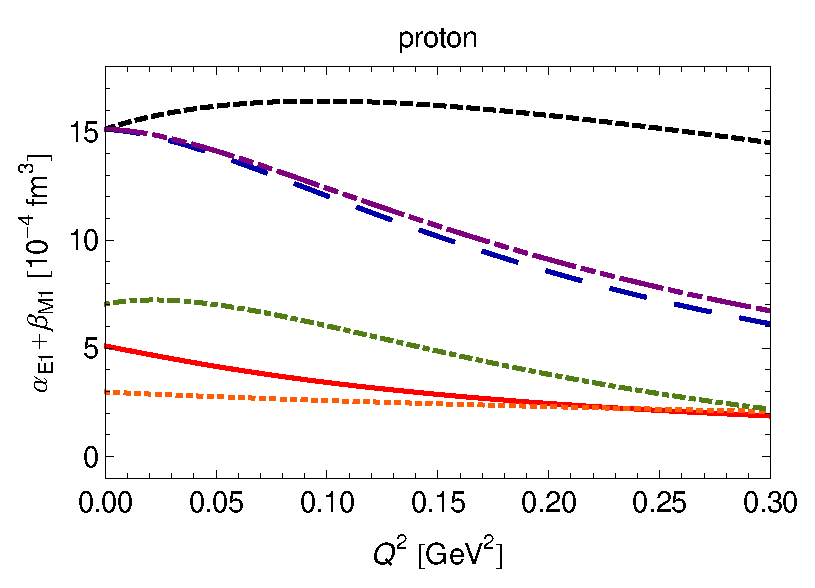
\epsfig{file=alpha+beta_p-orders-Dip.eps,width=9cm,angle=0}\\[0.5cm]
\hspace{-0.3cm}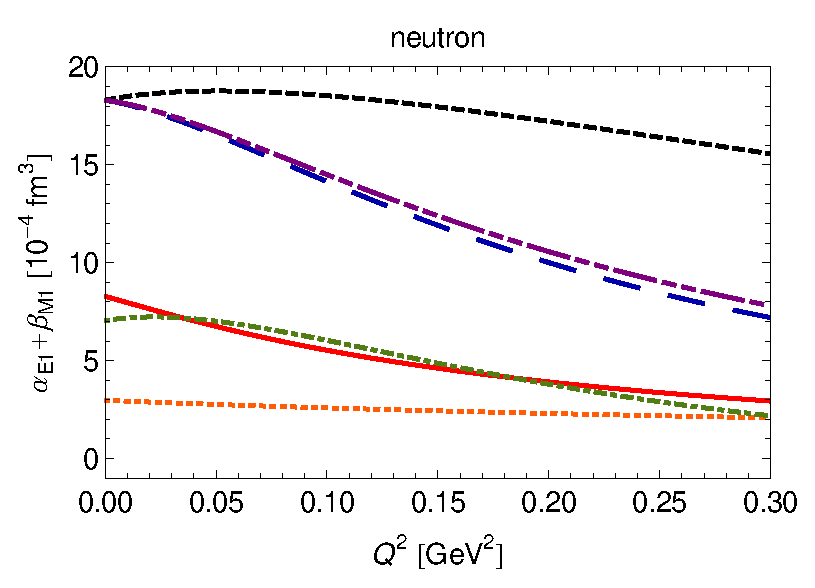
\epsfig{file=alpha+beta_n-orders-Dip.eps,width=9cm,angle=0} 
\caption{\small{Contributions of the different orders to the chiral prediction of $[\alpha_{E1}+\beta_{M1}](Q^2)$. Red short-dashed line: $\pi$-cloud contribution, green dot-dashed line: $\Delta$-exchange contribution, orange dotted line: $\pi \Delta$-loops contribution, blue solid line: total result, blue long-dashed line: total result without $g_C$ contribution, purple dot-dot-dashed line: total result without dipole.}\label{Fig:alpha+beta-orders}}
\end{center}
\end{figure}

\begin{figure}[H]
\begin{center}
\hspace{-0.3cm}\epsfig{file=alphaL_p-orders.eps,width=9cm,angle=0}\\[0.5cm] \hspace{-0.3cm}\epsfig{file=alphaL_n-orders.eps,width=9cm,angle=0} 
\caption{Contributions of the different orders to the chiral prediction of $\alpha_{L}(Q^2)$. The legend is the same as in Fig.~\ref{Fig:alpha+beta-orders}. \label{Fig:alphaL-orders}}
\end{center}
\end{figure}

\begin{figure}[H]
\begin{center}
\hspace{-0.3cm}\epsfig{file=gamma0_p-orders-Dip.eps,width=9cm,angle=0}\\[0.5cm] \hspace{-0.3cm}\epsfig{file=gamma0_n-orders-Dip.eps,width=9cm,angle=0} 
\caption{Contributions of the different orders to the chiral prediction of $\gamma_0(Q^2)$. The legend is the same as in Fig.~\ref{Fig:alpha+beta-orders}.  \label{Fig:gamma0-orders}}
\end{center}
\end{figure}
 
\begin{figure}[H]
\begin{center}
\hspace{-0.3cm}\epsfig{file=deltaLT_p-orders-Dip.eps,width=9cm,angle=0}\\[0.5cm] \hspace{-0.3cm}\epsfig{file=deltaLT_n-orders-Dip.eps,width=9cm,angle=0} 
\caption{Contributions of the different orders to the chiral prediction of $\delta_{LT}(Q^2)$. The legend is the same as in Fig.~\ref{Fig:alpha+beta-orders}.  \label{Fig:deltaLT-orders}}
\end{center}
\end{figure}

\begin{figure}[H]
\begin{center}
\hspace{-0.3cm}\epsfig{file=IAp-Dip-orders.eps,width=9cm,angle=0}\\[0.5cm]\hspace{-0.3cm}\epsfig{file=IAn-Dip-orders.eps,width=9cm,angle=0} 
\caption{Contributions of the different orders to the chiral prediction of $\Delta I_A(Q^2)$. The legend is the same as in Fig.~\ref{Fig:alpha+beta-orders}. The contribution of the elastic Pauli form factor is shown by the black long-long-short dashed line, where we used the form factor parametrization of Ref.~\cite{Bradford:2006yz}. \label{Fig:IA-orders-plot}}
\end{center}
\end{figure}

\begin{figure}[H]
\begin{center} 
\hspace{-0.3cm}\epsfig{file=I1p-Dip-orders.eps,width=9cm,angle=0}\\[0.5cm] \hspace{-0.3cm}\epsfig{file=I1n-Dip-orders.eps,width=9cm,angle=0} 
\caption{Contributions of the different orders to the chiral prediction of $\Delta I_1(Q^2)$. The legend is the same as in Fig.~\ref{Fig:IA-orders-plot}. \label{Fig:I1-orders-plot}}
\end{center}
\end{figure}

\begin{figure}[H]
\begin{center} 
\hspace{-0.3cm}\epsfig{file=d2p-Dip-orders.eps,width=9cm,angle=0}\\[0.5cm] \hspace{-0.3cm}\epsfig{file=d2n-Dip-orders.eps,width=9cm,angle=0} 
\caption{Contributions of the different orders to the chiral prediction of $\bar{d}_2(Q^2)$. The legend is the same as in Fig.~\ref{Fig:alpha+beta-orders}. \label{Fig:d2-orders-plot}}
\end{center}
\end{figure}

%\begin{figure}
%\begin{center}
%\epsfig{file=I1p-NoDip.eps,width=8cm,angle=0} \epsfig{file=I1n-NoDip.eps,width=8cm,angle=0} 
%\caption{Comparison of the full result without dipole (red solid line) with the rest of the available ChPT calculations for $I_{1}$. The blue solid line and its band is our total result with dipole, and the blue dashed line is the HB result (Ref.~\cite{Kao:2002cp}) and the grey band is the BChPT+$\Delta$ result of \cite{Bernard:2012hb}. The data are the same as in Fig~\ref{Fig:I1plot}.\label{Fig:I1-NoDip}}
%\end{center}
%\end{figure}


%\begin{figure}
%\begin{center}
%\epsfig{file=Gamma1p-NoDip.eps,width=8cm,angle=0} \epsfig{file=Gamma1n-NoDip.eps,width=8cm,angle=0} 
%\caption{Comparison of the full result without dipole (red solid line) with the rest of the available ChPT calculations for $\Gamma_{1}$. The blue solid line and its band is our total result with dipole, and the blue dashed line is the HB result (Ref.~\cite{Kao:2002cp}) and the grey band is the BChPT+$\Delta$ result of \cite{Bernard:2012hb}. The data are the same as in Fig~\ref{Fig:Gamma1plot}.\label{Fig:Gamma1-NoDip}}
%\end{center}
%\end{figure}


%\begin{figure}
%\begin{center}
%\epsfig{file=alpha+beta_p-NoDip.eps,width=8cm,angle=0} \epsfig{file=alpha+beta_n-NoDip.eps,width=8cm,angle=0} 
%\caption{Comparison of the full result without dipole (red solid line) with the rest of the available ChPT calculations for $\alpha+\beta$. The blue solid line and its band is our total result with dipole and the blue dashed line is the leading order result of \cite{Nevado:2007dd}. The data are the same as in Fig~\ref{Fig:alpha+betaplot}.\label{Fig:alpha+beta-NoDip}}
%\end{center}
%\end{figure}

%\begin{figure}
%\begin{center}
%\epsfig{file=IAp-NoDip.eps,width=8cm,angle=0} \epsfig{file=IAn-NoDip.eps,width=8cm,angle=0} 
%\caption{Comparison of the full result without dipole (red solid line) with the rest of the available ChPT calculations for $I_{A}$. The blue solid line and its band is our total result with dipole, and the blue dashed line is the HB result (Ref.~\cite{Kao:2002cp}) and the grey band is the BChPT+$\Delta$ result of \cite{Bernard:2012hb}. The data are the same as in Fig~\ref{Fig:IAplot}.\label{Fig:IA-NoDip}}
%\end{center}
%\end{figure}

%\begin{figure}
%\begin{center}
%\epsfig{file=d2p-NoDip.eps,width=8cm,angle=0} \epsfig{file=d2n-NoDip.eps,width=8cm,angle=0} 
%\caption{Comparison of the full result without dipole (red solid line) with the rest of the available ChPT calculations for $\bar{d}_{2}$. The blue solid line and its band is our total result with dipole, and the blue dashed line is the HB result (Ref.~\cite{Kao:2002cp}) and the grey band is the BChPT+$\Delta$ result of \cite{Bernard:2012hb}. The data are the same as in Fig~\ref{Fig:d2plot}.\label{Fig:d2-NoDip}}
%\end{center}
%\end{figure} 

%\begin{figure}
%\begin{center}
%\epsfig{file=deltaLT_p-NoDip.eps,width=8cm,angle=0} \epsfig{file=deltaLT_n-NoDip.eps,width=8cm,angle=0} 
%\caption{Comparison of the full result without dipole (red solid line) with the rest of the available ChPT calculations for $\delta_{LT}$. The blue solid line and its band is our total result with dipole, and the blue dashed line is the HB result (Ref.~\cite{Kao:2002cp}) and the grey band is the BChPT+$\Delta$ result of \cite{Bernard:2012hb}. The data are the same as in Fig~\ref{Fig:deltaLTplot}.\label{Fig:deltaLT-NoDip}}
%\end{center}
%\end{figure}

%\begin{figure}
%\begin{center}
%\epsfig{file=gamma0_p-NoDip.eps,width=8cm,angle=0} \epsfig{file=gamma0_n-NoDip.eps,width=8cm,angle=0} 
%\caption{Comparison of the full result without dipole (red solid line) with the rest of the available ChPT calculations for $\gamma_0$. The blue solid line and its band is our total result with dipole, the blue dashed line is the HB result (Ref.~\cite{Kao:2002cp}) and the grey band is the BChPT+$\Delta$ result of \cite{Bernard:2012hb}. The data are the same as in Fig~\ref{Fig:gamma0plot}.\label{Fig:gamma0-NoDip}}
%\end{center}
%\end{figure}


\end{document}